%%%%%%%%%%%%%%%%%%%%%%%%%%%%%%%%%%%%%%%%%%%%%%%%%%%%%%%%%%%%%%%%%%%%%%%%%%%%%%%%%%%%%%%%%%%%%%%%%%%%%
% This template is distributed with ABSOLUTELY NO WARRANTY.
% It serves as a guideline and constitutes a basic structure for a
% thesis/dissertation. The user assumes full responsibility for formatting
% and typesetting their document and for verifying that all the thesis
% requirements set by the University of Tennessee are met. Please refer to the most
% recent UT thesis guide (http://web.utk.edu/~thesis/thesisresources.shtml)
% or contact the thesis consultant (http://web.utk.edu/~thesis/).
% Please report any bugs to the thesis consultant.
%%%%%%%%%%%%%%%%%%%%%%%%%%%%%%%%%%%%%%%%%%%%%%%%%%%%%%%%%%%%%%%%%%%%%%%%%%%%%%%%%%%%%%%%%%%%%%%%%%%%%
% O P T I O N S:
% 1. thesis/dissertation
% 2. monochrome
% 3. all options provided by the report class
\documentclass[thesis,letterpaper,12pt]{utthesis} % thesis, one side
% some alternatives are:
%\documentclass[thesis,monochrome,letterpaper,12pt]{utthesis} %thesis, one side, monochrome text
%\documentclass[thesis,twoside,letterpaper,12pt]{utthesis} % thesis, two side
%\documentclass[thesis,monochrome,twoside,letterpaper,12pt]{utthesis} % thesis, two side, monochrome text
% for a dissertation, replace the thesis option by dissertation:
% \documentclass[dissertation,letterpaper,12pt]{utthesis} . . .
\renewcommand{\baselinestretch}{1.5} 	 % line Spacing
%%%%%%%%%%%%%%%%%%%%%%%%%%%%%%%%%%%%%%%%%%%%%%%%%%%%%%%%%%%%%%%%%%%%%%%%%%%%%%%%%%%%%%%%%%%%%%%%%%%%%
% TO DO: FILL IN YOUR INFORMATION BELOW - READ THIS SECTION CAREFULLY
%%%%%%%%%%%%%%%%%%%%%%%%%%%%%%%%%%%%%%%%%%%%%%%%%%%%%%%%%%%%%%%%%%%%%%%%%%%%%%%%%%%%%%%%%%%%%%%%%%%%%
\title{The EMC Effect in A=3 Nuclei}	       % title of thesis/dissertation
\author{Jason Bane}                % author's name
\copyrightYear{2018	}            % copyright year of your thesis/dissertation
\graduationMonth{December}           % month of graduation of your thesis/dissertation
\majorProfessor{Nadia Fomin}	    % advisor's name
\keywords{EMC, Nuclear Structure, Electron scatterning}	% keywords (optional) separated by commas - these are used in the PDF file properties
\viceProvost{Carolyn R. Hodges} % vice provost name
\major{Nuclear Physics}	% major: Mechanical Engineering, Aerospace Engineering, Mathematics...
\degree{Doctor of Philosophy}	    % degree: Doctor of Philosophy, Master of Science, Master of Engineering...
\college{Arts and Sciences}           % college
\dept{Physics and Astronomy}	% department
\university{The University  of Tennessee, Knoxville}	% school name
% THIS TEMPLATE ACCOMMODATES UP TO 5 COMMITTEE MEMBERS - ENTER ONLY THE NAMES OF THE MEMBERS ON YOUR COMMITTEE
\numberOfCommitteeMembers{4} % enter the number of committee members
\committeeMemberA {Jamie Coble}	% name of first committee member
\committeeMemberB {Kate Jones}	% name of second committee member
\committeeMemberC {Thomas Papenbrock}	% ... you get the trend!
\committeeMemberD {Soren Soreson}	% if your committee has less than 4 members, you do not need to edit the
\committeeMemberE {Committee Member 5}  % rest of committee names
%%%%%%%%%%%%%%%%%%%%%%%%%%%%%%%%%%%%%%%%%%%%%%%%%%%%%%%%%%%%%%%%%%%%%%%%%%%%%%%%%%%%%%%%%%%%%%%%%%%%%
% LOAD SOME USEFUL PACKAGES
%%%%%%%%%%%%%%%%%%%%%%%%%%%%%%%%%%%%%%%%%%%%%%%%%%%%%%%%%%%%%%%%%%%%%%%%%%%%%%%%%%%%%%%%%%%%%%%%%%%%%
\usepackage{nomencl}                    % produces a nomenclature
\usepackage{float}                      % figure floats
\usepackage{natbib}                     % this package allows you to link your references
\usepackage{graphicx}					% graphics package
\graphicspath {{images/}} % specify the path where figures are located
\usepackage{fancyhdr}                   % fancy headers and footers
\usepackage{url}                      % nicely format url breaks
\usepackage[inactive]{srcltx}		 	% necessary to use forward and inverse searching in DVI
\usepackage{relsize}                    % font sizing hierarchy
\usepackage{booktabs}                   % professional looking tables
\usepackage[config, labelfont={bf}]{caption,subfig} % nice sub figures
\usepackage{tikz}
\usepackage{multicol}
%\usepackage{floatrow}
\usepackage[outdir=./images/]{epstopdf}
%%/lin\usepackage{csvsimple}

\usepackage{lineno}
%\linenumbers
\usepackage{mathrsfs}                   % additional math scripts
%%% PACKAGES THAT ARE PRELOADED WITH THE CLASS ARE: amsmath,amsthm,amssymb,setspace,geometry,hyperref,and color
%%%%%%%%%%%%%%%%%%%%%%%%%%%%%%%%%%%%%%%%%%%%%%%%%%%%%%%%%%%%%%%%%%%%%%%%%%%%%%%%%%%%%%%%%%%%%%%%%%%%%
\begin{document}
    \pagenumbering{alph} % this is needed to clear certain issues with the hyperref package
    %
    \makeApprovalPage % make the approval page - this is the page that needs to be signed & returned to the thesis/dissertation consultant
    \makeETDApprovalPage % make the Electronic Thesis & Dissertation page - this page is kept with the electronic copy
    %
    \addToPDFBookmarks{0}{Front Matter}{rootNode} % create a root node named "Front Matter" in the pdf bookmarks
    \addToPDFBookmarks{1}{Title}{a} % add a pdf bookmark to the title page
    \makeTitlePage % make the title page. Make sure you properly set the \docType
    %
    \pagenumbering{roman}
    \setcounter{page}{2}
    %
    \makeCopyrightPage % make the copyright page
    %
    \addToPDFBookmarks{1}{Dedication}{b} % add a pdf bookmark to the dedication page
    \include{front-matter/dedication} % include the dedication
    %
    \addToPDFBookmarks{1}{Acknowledgements}{c} % add a pdf bookmark to the acknowledgements page
    \begin{center}
	{\large \textbf{Acknowledgments}}\\
\end{center}


\paragraph{}I would like to thank everybody that played a role in completing this step of my life. I know there is no way that I could go one by one through every person that helped and thank them. I am sure that it would take too many pages and then I would leave somebody out. There are a few special people, that I would like to call out. 
\paragraph{}First, I would like to thank my brother, James for the courage to change career paths and my parents, Barb, Howard, and Deb for the support and guidance. Thanks to Dallas and Jennifer, for housing me for a few months. Thank you Dr. Fomin for targeting my weakness, the beach, and giving me the chance to join the JLab community. Also, I would like to thank Dr. Fomin for supporting my research and guiding me though the swamps of PhD. research. I would like to thank the JLab community specially Dr. Higinbotham for accepting me into the community and helping through this journey including keeping the office door open for me to drop in a million times! I would also like to thank my committee for guiding me through my defense and allowing me to graduate. 
\paragraph{}I would really like to thank the extended tritium family of grad students and post docs. Working with such a great group of people from around the world has truly been amazing!! Thank you, Sheren, Scott, Jessica, Tyler H., Hanjie, Dien, Mike, Tong, Shujie, Rey, Johnathan, Tyler K., Nathaly, Bishnu, Evan, Florian, Luke, Marco, and Zhihong. Lastly and I think the person deserving of the most thanks, is my wife, Callie. Thank you so much for everything! Specially thank you for dropping everything and coming on this adventure with me!.

\paragraph{}I would like to thank the DOE and JSA for financial support throughout my time at JLab.  % include the acknowledgements
    %
    \addToPDFBookmarks{1}{Quote}{d} % add a pdf bookmark to the quotation page
    \include{front-matter/quote} % include a quote
    %
    \addToPDFBookmarks{1}{Abstract}{e} % add a pdf bookmark to the abstract page
    \begin{abstract}
The European Muon Collaboration(EMC) discovered an unexpected and puzzling result in 1983 when comparing the deep inelastic scattering(DIS) nuclear structure functions of Deuterium and Iron. The larger than expected structure function for Deuterium compared to the large nuclei of  Iron was coined the EMC effect and has been studied for nearly four decades. Experiments at CERN, Stanford (SLAC), Thomas Jefferson National Accelerator Facility(JLab), and other labs have studied the EMC effect for a range of different nuclei, attempting to complete a part of the EMC puzzle. I will discuss recent results from JLab exploring the EMC effect by using an electron beam to probe two mirror nuclei, Helium-3 and Tritium. 
\end{abstract} % your abstract
    %
    \addToPDFBookmarks{0}{Table of Contents}{f}
    \tableofcontents % generate a table of contents
    %
    \addToTOC{List of Tables} % this will add the list of tables to the Table of Contents (TOC)
    \listoftables % generate a list of tables
    %
    \addToTOC{List of Figures} % this will add the list of figures to the Table of Contents (TOC)
    \listoffigures % generate a list of figures
    %
    \makenomenclature % OPTIONAL
    \addToPDFBookmarks{0}{Nomenclature}{g} % OPTIONAL
    \printnomenclature[1.25in] % OPTIONAL
    %
    \newpage
    \pagenumbering{arabic}
    \setcounter{page}{1}
    %%%%%%%%%%%%%%%%%%%%%%%%%%%%%%%%%%%%%%%%%%%%%%%%%%%%%%%%%%%%%%%%%%%%%%%%%%%%%%%%%%%%%%%%%%%%%%%%%%%%%
    % INCLUDE THE CHAPTERS STARTING WITH THE NOMENCLATURE IF PRESENT
    %%%%%%%%%%%%%%%%%%%%%%%%%%%%%%%%%%%%%%%%%%%%%%%%%%%%%%%%%%%%%%%%%%%%%%%%%%%%%%%%%%%%%%%%%%%%%%%%%%%%%
						
     	


\chapter{Introduction}\paragraph{}Understanding the world around us is the goal of every scientist, from the chemist that experiments with the formation of atoms to the geologist exploring the process of rock formations. Nuclear physicists focus on studying the fundamental constituents of matter, the building blocks of nature. Physicist use scattering experiments at accelerator facilities, like CERN in Switzerland, DESY in Germany, BATES in Massachusetts, JLAB in Virgina, and many others, to study the protons and neutrons and their constituents that make up a nucleus. These experiments allow physicists to observe the internal structure of the nucleus and to investigate the interactions between the quarks and gluons. Many of the experiments are design to confirm a existing results while also expanding on unique ideas.
\paragraph{}In the last century, there have been numerous breakthroughs in the fields of nuclear and particle physics. Rutherford discovered the proton by bombarding light nuclei with alpha particles to produce 
	\begin{equation}
	^{14}N + ^4He \rightarrow ^{17}O + p.
	\end{equation}
This reaction allowed Rutherford to conclude that the Hydrogen nucleus was a constituent of an atomic nuclei \cite{PnN}. In the late 1950s, experimental results published by W. McAllister and R. Hofstadter exposed some of the eternal structure of the proton \cite{Flay,Hof}. The European Muon Collaboration(EMC) produced results in the early 1980s showing a differences between the internal structure of the deuterium nucleus and Iron \cite{seeley,CC}. The data received from scattering experiments using alpha particles contain information about the target, the beam, and the interaction between the two. Deciphering and analyzing this data can be convoluted because the cross-section contains information about the internal structure of the target and the beam along with the interaction and forces between the two \cite{PnN}.  

\section{Electron scattering}
\paragraph{} In order to remove some of the complexity in scattering experiments, one may employ highly relativistic electrons. Electrons being point-like particles without any internal structure allow the elimination of some of the analysis difficulties with using alpha particles in scattering experiments due to their complex internal structure. Electrons and the target nucleus, nucleon, or quarks interact via the exchange of a virtual photon. Using quantum electrodynamics (QED), these interactions can accurately be described by the well known electromagnetic interaction. Higher order terms of this process contribute very little due to the coupling constant $\alpha \approx 1/137 $, being much smaller than one. 
\paragraph{} Figure \ref{feynman} represents an electron scattering from a proton. The incoming or incident electron's four-momentum is described as k = (E,$ \vec{k}$) and the scattering electron's four-momentum is represented by $k^\prime{}$ = ($E^\prime{}$,$\vec{k}^\prime{}$). The exchange of the virtual photon in this electromagnetic interaction is defined by the four-momentum transfer q: 
\begin{equation}
\label{Q}
Q^2 \equiv -q^2 = 4EE^\prime{} sin^2(\theta/2).
\end{equation} 
In equation \ref{Q}, E and E$^\prime$ are the electron energy before and after the scattering interaction. Theta is the angle that describes the deflection of E$^\prime$ from the electron's original path. 

\begin{figure}[h]
\centering
\caption{Simple Feynman diagram of an electron scattering from a proton \cite{Flay}.}
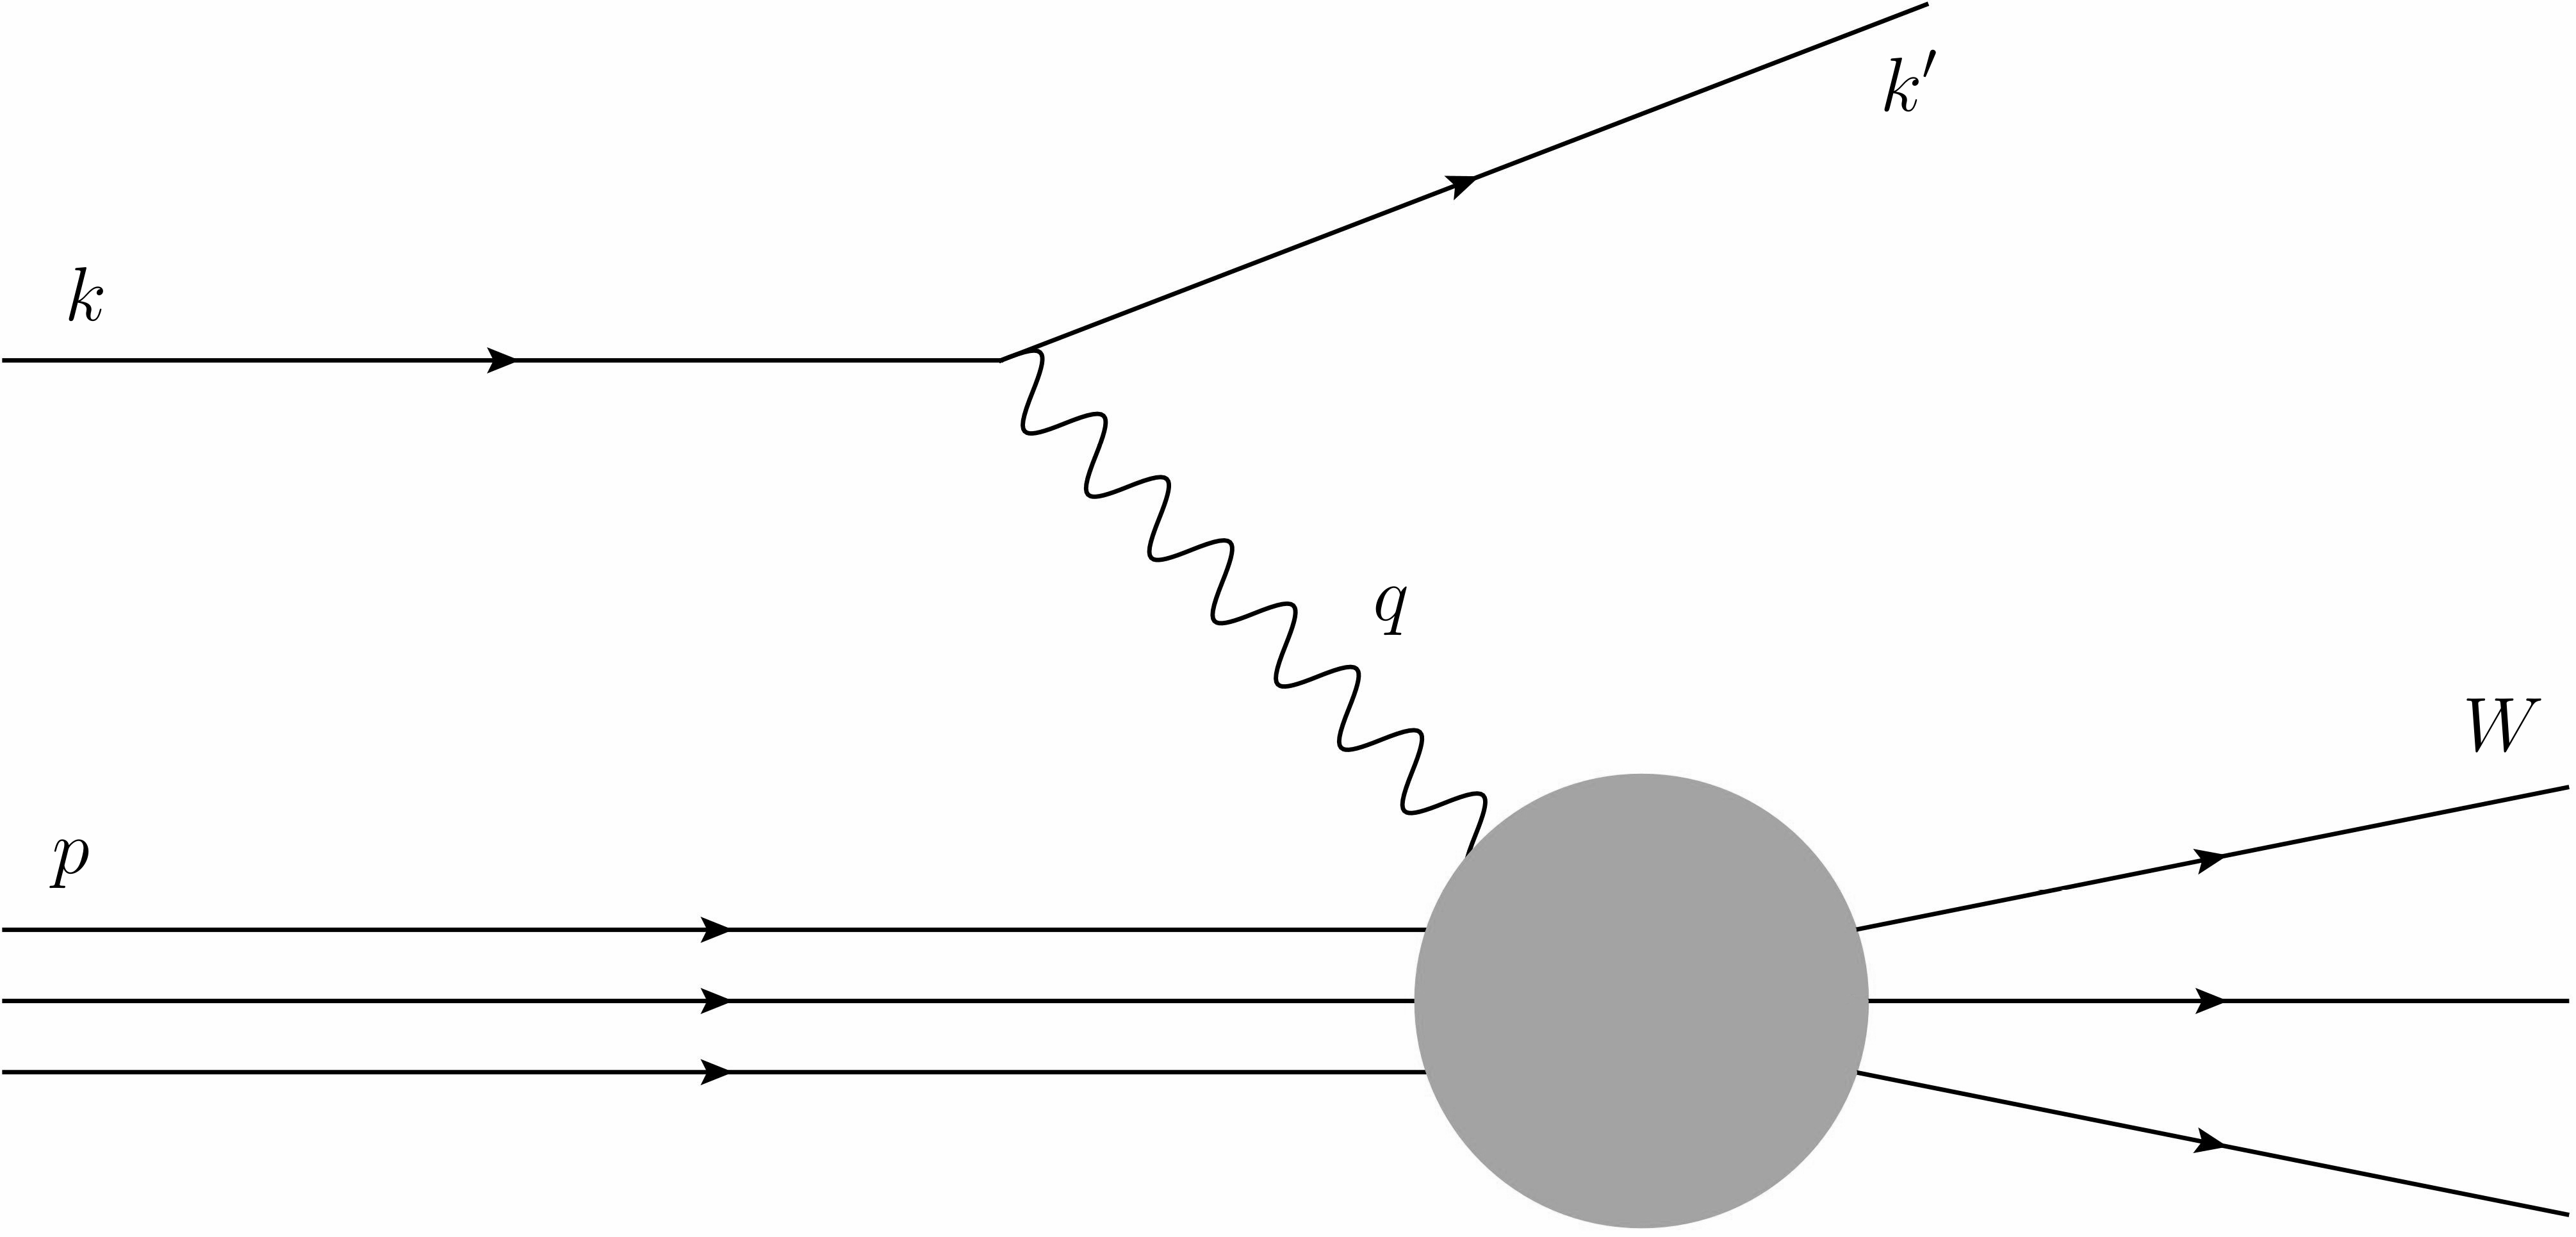
\includegraphics[width=10cm]{feyman_e_p.png}
\label{feynman}
\end{figure}
Along with $Q^2$, the variables $\nu$, W, and$x_B$  are used to narrate the evolution of the electron scattering process. $\nu$, defined as $p\cdot q/M$. In the rest frame of the target,  $\nu$ can be described by:

\begin{equation}
\label{v}
\nu = E - E^\prime{}.
\end{equation}
Simply, $\nu$ is the magnitude of energy loss by the electron during the scattering interaction. The invariant mass of the system, W,  defines the hadronic state produced by the scattering event. 
\begin{equation}
\label{W}
W^2 \equiv (q + p)^2 = M^2 + 2M\nu -Q^2.
\end{equation}
A scattering event with the invariant mass equal to the square of the mass of the nucleon, ($M^2$), falls in the regime of elastic scattering. W above $M^2$ will transform the scattering interaction from an elastic scattering to inelastic scattering due to the excited state of the scattered byproduct. $x_B$, the Bjorken scaling variable is a dimensionless quantity that measures the inelastically of a scattering process. $x_B$ is defined as: $x := \frac{Q^2}{2M\nu}$.
\paragraph{} The intrinsic likelihood of an event with a certain $Q^2$, $\nu$, and $W$ is defined by the scattering cross section. An electron scattering off of a target with a charge of $Z*e$ can be described by the Rutherford cross-section. Povh et. al. details the Rutherford cross section as:
\begin{equation}
\bigg(\frac{d\sigma}{d\Omega}\bigg)_{Rutherford} = \frac{ \big(zZe^2\big)^2} {\big( 4\pi \epsilon_0\big)^2 * \big(e E_{kin}\big)^2 sin^4\big( \theta / 2 \big) }. 
\end{equation}
  In the early 1920s, German physicists Stern and Gerlach performed an experiment that confirmed the presence of electron angular momentum. Later a discovery of electron spin was made by Uhlenbeck an Gloudsmit.  The Rutherford cross-section neglects the spin of a electron and it's target. The Mott cross-section is the evolved version of the Rutherford cross-section. It has been modified to include the intrinsic spin of the target and electron. The Mott cross-section is: \cite{HighE,PnN}
\begin{equation}
\bigg(\frac{d\sigma}{d\Omega}\bigg)_{Mott} = \frac{4Z^2\alpha^2 \big(\hbar c \big)^2 E{^{\prime} }^2}{ |\boldsymbol{q}c|^4} cos^2 (\theta/2).
\end{equation}

\paragraph{}There is an agreement between the measured cross section and the theoretical Mott cross-section when in the limit of $|\boldsymbol{q}| \rightarrow  0$ for scattering events of electrons off of a target nuclei. As $|\boldsymbol{q}|$ climbs furtherer from zero, the experimentally measured cross sections systematically decreases \cite{PnN}. Increasing the $|\boldsymbol{q}|$ of an interaction reduces the size of the wavelength of the virtual photon that mediates the electromagnetic interaction between the electron and target nuclei and increases the resolution of the probe. The wavelength of this virtual photon is inversely proportional to $|\boldsymbol{q}|$, and can be described by the following: $\lambda = \ \frac{\hbar}{|\boldsymbol{q}|}$ \cite{PnN}. Increasing the amount of momentum transfered in an electromagnetic reaction allows one to study deeper into the nucleus. 
\paragraph{} Studying the internal structure of a nucleus with the electromagnetic interaction requires increasing the momentum transfered. Pushing $|\boldsymbol{q}|$ to be comparable with the mass of a nucleon adds more complexity to the details of the scattering interaction. At the appropriate levels of $|\boldsymbol{q}|$ to study the nucleons in the nucleus, the Mott cross-section equation requires modifications to include additional factors that incorporate information about the target. The Rosenbluth formula is based on the Mott cross section and embraces target recoil, magnetic moment, and charge and current distributions. Povh writes the Rosenbluth formula as:
\begin{equation}
\label{rosen}
\bigg(\frac{d\sigma}{d\Omega}\bigg)=\bigg(\frac{d\sigma}{d\Omega}\bigg)_{Mott} *\bigg\lbrack \frac{G^2_E(Q^2) +\tau G^2_M(Q^2)}{1+\tau} + 2\tau G^2_M(Q^2)tan^2\frac{\theta}{2} \bigg\rbrack.
\end{equation}
Equation \ref{rosen} contains $G^2_E(Q^2)$ and $G^2_M(Q^2)$, the electric and magnetic form factors. $\tau$ is used in the Rosenbluth formalism to account for the magnetic moment of a nucleon and is defined as: $\tau = \frac{Q^2}{4M^2c^2}$ \cite{PnN}. In the general case of electron scattering off of a free proton or neutron elastically, the scattered energy of the electron will be a function of the incident electron's energy and the scatted angle of the electron, shown in the following equation.
\begin{equation}
E^\prime =\frac{E}{1+\frac{E}{Mc^2}(1-cos\theta)}
\end{equation}
\subsection{Deep inelastic scattering}
\paragraph{}The first generation of electron scattering experiments achieving a significantly large  $|\boldsymbol{q}|$ used a linear accelerator with a 25 GeV maximum beam energy, and following generations increased the total interaction energy to substantially higher thresholds. At these high incident beam energies, individual resonances cannot be separated in the invariant mass spectrum above 2.5 GeV. Observations made into this convoluted invariant mass spectrum has shown that many strongly interacting particles are produced, known as hadrons. Scattering interactions that generate these hadrons are considered to be inelastic. Inelastic scattering events contain the possibility of conceiving additional resultants and increase the complexity of a scattering interaction. Inelastic scattering events occur when the wavelength of the virtual photon is comparable to the radius of the struck nucleon or when $Q^2R^2 \lesssim 1$\cite{PnN}. Increasing the amount of transferred momentum so that $Q^2R^2 \gtrsim 1$, increase the resolution of the probe to a level that allows for the interacting with the charge constituents within the nucleon. When the scattering event probes the fundamental elements of a nucleon, the scattering process is titled deep inelastic scattering(DIS). Due to the increase in complexity, an additional degree of freedom has to be included in the scattering cross section equation. Modifying the Rosenbluth formula to include the inelastic scattering structure functions $F_1(Q^2,\nu)$ and $F_2(Q^2,\nu)$ evolves the Rosenbluth formula to contain the needed complexity of an inelastic event. These modifications are shown in equation \ref{ISCS}.
\begin{equation}
\label{ISCS}
\frac{d^2\sigma}{d\Omega dE^\prime}=\bigg(\frac{d\sigma}{d\Omega}\bigg)_{Mott} \bigg\lbrack \frac{F_2(Q^2,\nu)}{\nu} + \frac{2F_1(Q^2,\nu)}{M}tan^2\frac{\theta}{2} \bigg \rbrack
\end{equation}  


	\cite{DISearly}
	\cite{DISproton}

	
\section{EMC Effect}
\paragraph{}The European Muon Collaboration (EMC) performed a deep inelastic measurement with 120-280 GeV muons on iron and deuteron targets \cite{challenge}. The EMC extracted A/D structure function ratios versus the Bjorken scaling variable, $x$.  The relationship originally expected by the EMC contained the sum of the structure functions of each nucleon in a nucleus. Each nucleus has a certain number of neutrons (N) and a amount of protons (Z). The expected structure function for a nucleus could be written as:
\begin{equation}
F_A = N F_2^N + ZF_2^P.
\end{equation}
 The EMC compared the extracted structure functions from iron and deuterium. Their results are shown in Figure \ref{EMCOld}. The $\frac{A}{D}$ structure function ratio showed an unexpected downward slope. This phenomenon was titled the EMC effect. This finding demonstrated to the EMC that their understanding of the nucleus was incorrect. A nucleon's structure function and thereby, the constituent quark distributions may be altered by the nucleus. 
\begin{figure}[h]
\centering
 \caption{ Graph of the ratio of A/D structure functions vs $x$ for Carbon \cite{CC}.}
 \label{EMCOld}
 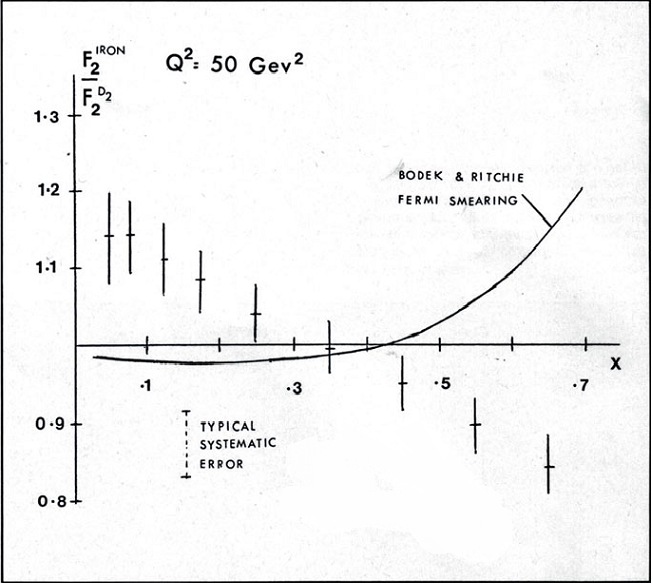
\includegraphics[width=10cm]{EMC.png} 
 \end{figure} 

\paragraph{}Ever since the European Muon Collaboration discovered the depletion of quarks at high $x$ for A $>$2 nuclei, physicists have tried to discover its cause. Scientists at SLAC extracted structure function ratios for many nuclei including; $^4$He, $^9$Be, $^{12}$C, $^{27}$Al, $^{40}$Ca, $^{56}$Fe, $^{108}$Ag, and $^{197}$Au. There were slightly different results for each nucleus. The magnitude of the EMC effect, taken to be the A/D ratio at $x=0.6$, was found to be different for the various nuclei, and roughly scaled with the size or density of the nuclei. The NMC (New Muon collaboration), another group at CERN, gathered precise data in order to construct the inclusive cross section of deuterium and protons. BCDMS collaboration extracted data for N and Fe structure function ratios. Figure \ref{EMC3} shows some of the data from SLAC and BCDMS on the EMC effect for Iron and Cu. Figure \ref{EMC 1} shows this result from a recent JLab EMC measurement, most precise to date. Many models over the years have been able to reproduce the shape of the A/D ratios. These models can contain traditional nuclear physics effects like momentum distribution or pion-charge contributions. Some models also describe the EMC effect through quark momentum distribution or modification of the internal structure \cite{Norton, piler, arri, DF, gomez}. However, no single model has provided a complete picture of the possible underlying physics. Precise data from Jlab's E03-103 experiment has revitalized this research. This experiment focused on precision measurements in light nuclei and added $^{3}$He as a target nucleus. Instead of taking the A/D ratio at a certain $x$-value to be the magnitude of the EMC effect, this analysis looked at the slope instead. This eliminated sensitivity to normalization uncertainties.

\begin{figure}[h]
\centering
\caption{EMC effect from EMC, SLAC, and BCDMS \cite{Norton}}
\label{EMC3}
\centering
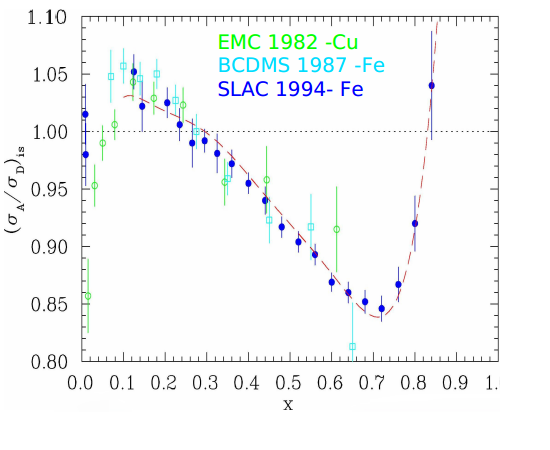
\includegraphics[width=10cm]{EMC3.png}
\end{figure}

\begin{figure}[h]
\centering
 \caption{ Graph of the ratio of A/D structure functions vs $x$ for Carbon \cite{CC}.}
 \label{EMC 1}
 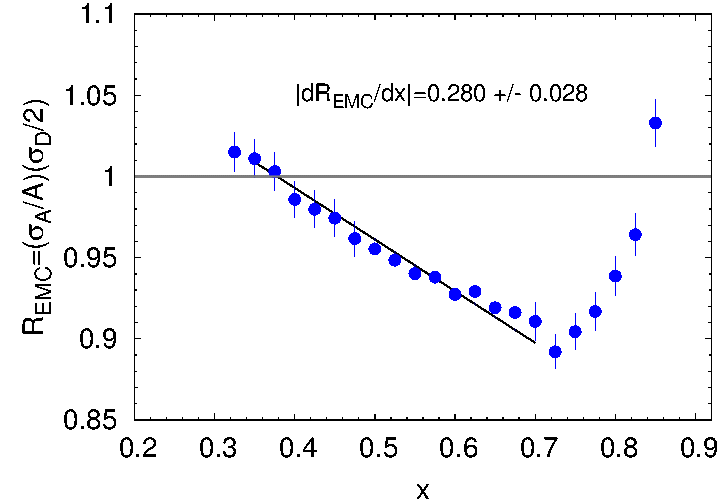
\includegraphics[width=10cm]{EMC1.png} 
 \end{figure} 
 

\paragraph{} In Figure , $^9$Be was found not to follow the previously observed scaling with nuclear density. This result from Jefferson Lab determined that the previous idea of a dependence on A or nuclear density in the EMC effect to be incorrect \cite{seeley}. This result spawned a drive to determine another explanation for the EMC effect and understand what clue the $^9$Be outlier was providing. The structure of this nucleus is made up of two high-density alpha particles and a single neutron \cite{ajppt}. The regions of higher density that are contained in a comparatively large volume may be able to explain why $^9$Be does not follow the expected trend. This suggests that the EMC effect could be a function of local nuclear density \cite{seeley}. 




\section{MARATHON}
Experiment E12-010-102, MARATHON (MeAsurement of the $F2^n$/$F_2^p$,$d$/$u$ RAtios and A=3 EMC Effect in Deep Inelastic Electron Scattering Off the Tritium and Helium MirrOr Nuclei), will use deep inelastic scattering off of the mirror nuclei $^3$H and $^3$He to measure the EMC effect for both $^3$H and $^3$He, to determine the ratio of the neutron to proton inelastic structure functions, and to find the ratio of the down to up quark distributions in the nucleon.


    	\chapter{EMC Effect}	
\section{European Muon Collaboration}\label{sec:EMC}
\paragraph{}The European Muon Collaboration (EMC) performed a deep inelastic measurement with 120-280 GeV muons on iron and deuteron targets \cite{challenge}. The EMC studied the per nucleon normalized Fe/D structure function ratio versus the Bjorken scaling variable, $x$. The EMC expectations for this ratio originally was unity for $x$ between 0.05 and 0.7 \cite{CC}. The reasoning for this expectation was the belief that at large magnitude of $Q^2$ the interaction between protons and neutrons would not contribute to the total structure function of the nucleus. This was the understanding because the binding energy of a few MeV would not interferer with GeV scale of the DIS interaction \cite{Ajth}. The expected structure function for a nucleus could be written as:
\begin{equation}
F_2^A = N F_2^N + ZF_2^P.
\end{equation}
In this quasi-free nucleon picture, the nucleons are used to build up the nuclear structure ($F_2^A$) by summing up the neutron structure function ($F_2^N$) with the proton structure function($F_2^P$) for each nucleon. 



The EMC compared the extracted structure functions from iron and deuterium. Their results are shown in Figure \ref{EMCOld}. The $\frac{A}{D}$ structure function ratio showed an unexpected downward slope. This phenomenon was titled the EMC effect. This finding demonstrated to the EMC that their understanding of the nucleus was incorrect. A nucleon's structure function and thereby, the constituent quark distributions may be altered by the nucleus. 
\begin{figure}[h]
	\centering
	\caption{ Graph of the ratio of A/D structure functions vs $x$ from the EMC. \cite{CC,EM}.}
	\label{EMCOld}
	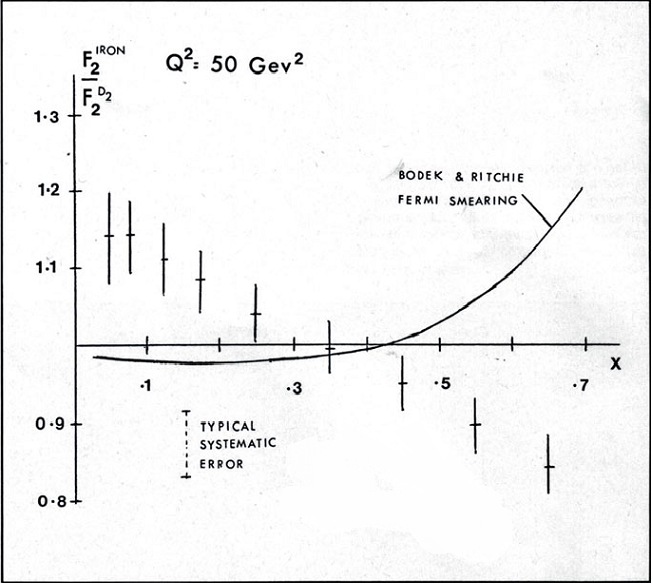
\includegraphics[width=10cm]{EMC.png} 
\end{figure} 

\paragraph{}Ever since the European Muon Collaboration discovered the depletion of quarks at high $x$ for A $>$2 nuclei, physicists have tried to discover its cause. Scientists at SLAC extracted structure function ratios for many nuclei including; $^4$He, $^9$Be, $^{12}$C, $^{27}$Al, $^{40}$Ca, $^{56}$Fe, $^{108}$Ag, and $^{197}$Au. There were slightly different results for each nucleus. The magnitude of the EMC effect, taken to be the A/D ratio at $x=0.6$, was found to be different for the various nuclei, and roughly scaled with the size or density of the nuclei. The NMC (New Muon collaboration), another group at CERN, gathered precise data in order to construct the inclusive cross section of deuterium and protons. BCDMS collaboration extracted data for N and Fe structure function ratios. Figure \ref{EMC3} shows some of the data from SLAC and BCDMS on the EMC effect for Iron and Cu. Figure \ref{EMC 1} shows this result from a recent JLab EMC measurement, most precise to date. Many models over the years have been able to reproduce the shape of the A/D ratios. These models can contain traditional nuclear physics effects like momentum distribution or pion-charge contributions. Some models also describe the EMC effect through quark momentum distribution or modification of the internal structure \cite{Norton, piler, arri, DF, gomez}. However, no single model has provided a complete picture of the possible underlying physics. Precise data from Jlab's E03-103 experiment has revitalized this research. This experiment focused on precision measurements in light nuclei and added $^{3}$He as a target nucleus. Instead of taking the A/D ratio at a certain $x$-value to be the magnitude of the EMC effect, this analysis looked at the slope instead. This eliminated sensitivity to normalization uncertainties.

\begin{figure}[h]
\centering
\caption{EMC effect from EMC, SLAC, and BCDMS \cite{Norton}}
\label{EMC3}
\centering
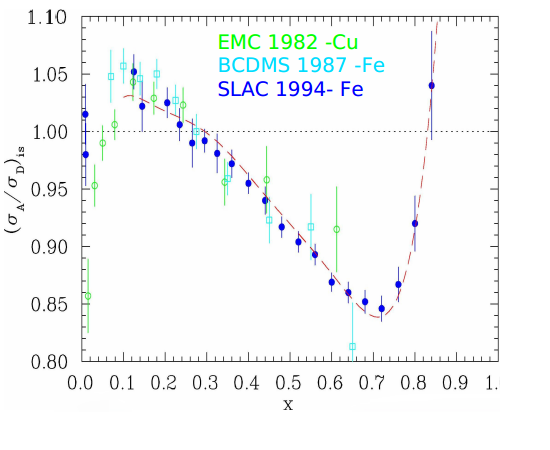
\includegraphics[width=10cm]{EMC3.png}
\end{figure}

\begin{figure}[h]
\centering
 \caption{ Graph of the ratio of A/D structure functions vs $x$ for Carbon \cite{CC}.}
 \label{EMC 1}
 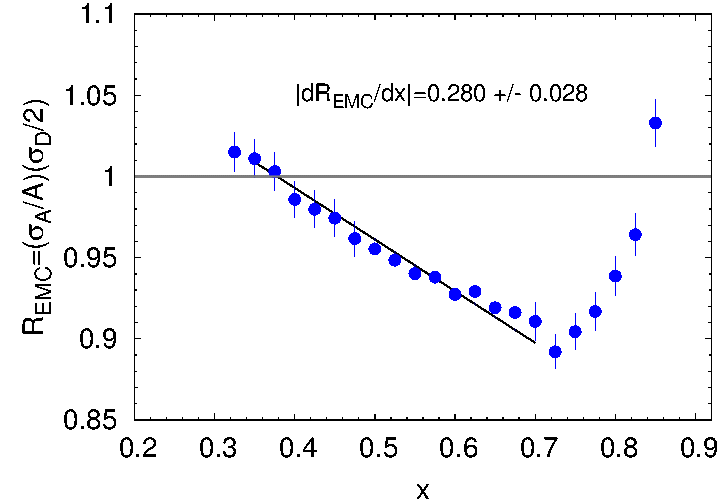
\includegraphics[width=10cm]{EMC1.png} 
 \end{figure} 
 

\paragraph{} In Figure , $^9$Be was found not to follow the previously observed scaling with nuclear density. This result from Jefferson Lab determined that the previous idea of a dependence on A or nuclear density in the EMC effect to be incorrect \cite{seeley}. This result spawned a drive to determine another explanation for the EMC effect and understand what clue the $^9$Be outlier was providing. The structure of this nucleus is made up of two high-density alpha particles and a single neutron \cite{ajppt}. The regions of higher density that are contained in a comparatively large volume may be able to explain why $^9$Be does not follow the expected trend. This suggests that the EMC effect could be a function of local nuclear density \cite{seeley}. 




\section{MARATHON}
Experiment E12-010-102, MARATHON (MeAsurement of the $F2^n$/$F_2^p$,$d$/$u$ RAtios and A=3 EMC Effect in Deep Inelastic Electron Scattering Off the Tritium and Helium MirrOr Nuclei), will use deep inelastic scattering off of the mirror nuclei $^3$H and $^3$He to measure the EMC effect for both $^3$H and $^3$He, to determine the ratio of the neutron to proton inelastic structure functions, and to find the ratio of the down to up quark distributions in the nucleon.


    	


\chapter{ Experimental Setup}

\section{Thomas Jefferson Lab}
\paragraph{}Thomas Jefferson Lab (Jlab) in Newport News, Virgina hosted the MARATHON experiment in the Fall of 2017 and Spring of 2018. Jlab uses support from the U.S. Department of Energy(DOE) and the state of Virgina to complete the lab's mission of delivering productive research by exploring the atomic nucleus and its fundamental constituents, including precise tests of their interactions. Along with applying an advanced particle accelerator, particle detectors and other technologies to develop new basic research capabilities and to address the challenges of a modern society.
	\subsection{CEBAF}
	\paragraph{}The Continuous Electron Beam Accelerator Facility (CEBAF) was recently upgraded to a 12 GeV accelerator, upgrading it to be able to supply a 11 GeV beam of continuous electrons of up to 200 $\mu$A of current to three experimental halls (A,B,C) and 12 GeV to the recently constructed hall D. After being accelerated to 45 MeV by a polarized electron gun or a thermionic injector, the electrons are injected into the North linear accelerator (LINAC), shown in figure \ref{CEBAF}. The polarized gun can supply electrons with up to 80$\%$ polarization and the polarization direction can be controlled by a wien filter. To ensure the level of polarization, a 5 MeV Mott polarimeter may be used to measure the level of polarization\cite{HallA}.
	\paragraph{} The electrons are conveyed through two LINACs and two bending arcs per complete pass of the accelerator. Electrons traveling to Halls A, B, and C complete a maximum of four and a half revolutions around the accelerator. Electrons going to all D travel through the north LINAC for an extra boost. These particles receive approximately 2.2 GeV in energy for each cycle through the accelerator. The radio frequency (RF) cavities in each LINAC use an oscillating electromagnetic field to supply a force to accelerate the passing electrons. These Niobium RF cavities are cooled to 2 K in order to create conditions that allow the cavities to be superconducting \cite{HallA}.    
	
	\begin{figure}[h]
	\centering
	 \caption{Schematic Layout of CEBAF. }
	 \label{CEBAF}
	 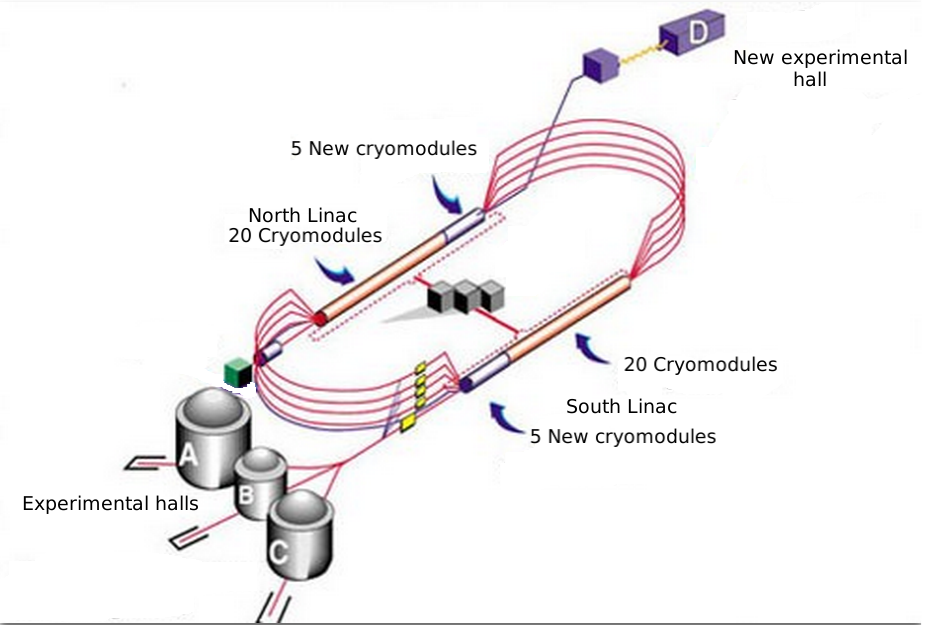
\includegraphics[width=10cm]{CEBAF.png} 
	 \end{figure} 
	 
	 \subsection{Hall A}
	 
	\begin{figure}[H]
		\centering
		\caption{A 3D drawing of Hall A. }
		\label{HallA}
		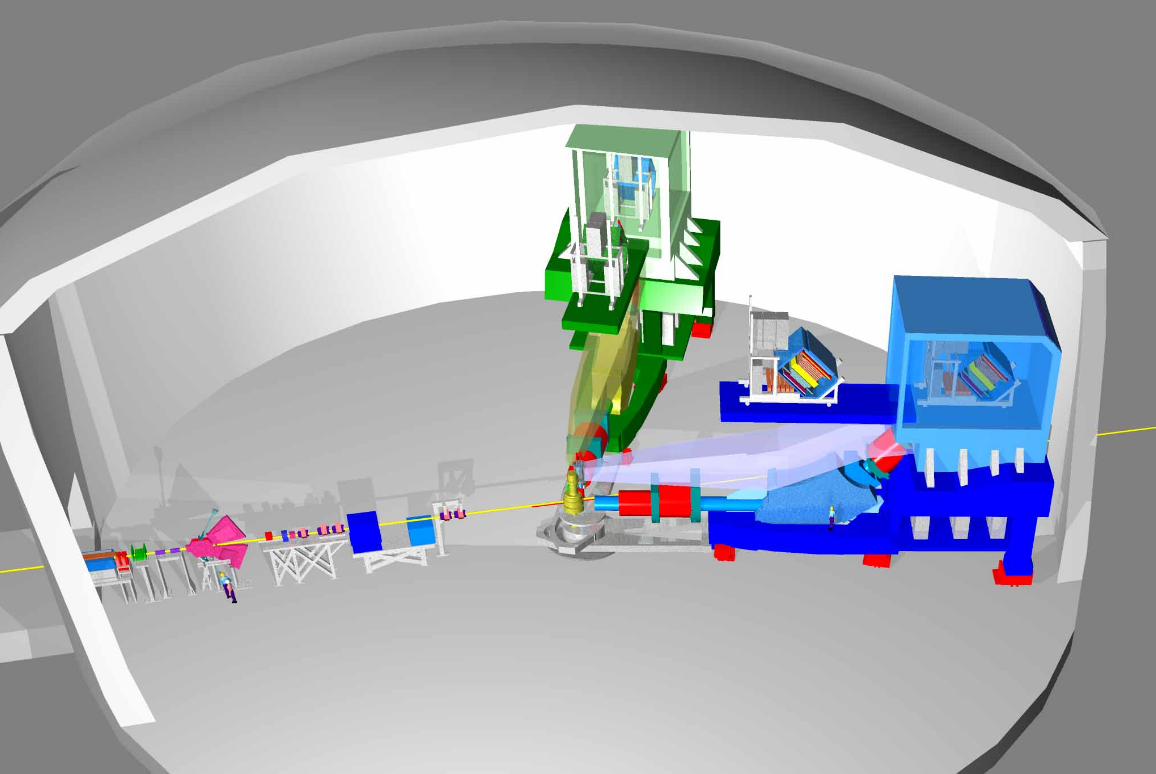
\includegraphics[width=14cm]{HallA_2.png} 
	\end{figure} 	 
	 
	 \paragraph{}The experimental Hall A and the scientific equipment used were designed for detailed investigations of the internal structure of nuclei. Two high resolution spectrometers in Hall A use the inclusive (e,e$\prime$) and exclusive (e,e$\prime$ p) reactions to gain a greater understanding of the structure of the nucleus. Completing detailed studies with high resolution and extreme accuracy requires knowing the beam position, size, energy, current, direction, and polarization when the beam strikes the target. The instrumentation used in the precise measurement of these quantities in Hall A  are shown in figure \ref{BeamLine} \cite{HallA}.

	 \paragraph{} A pair of Beam Position Monitors(BPM)s are used to measure the relative beam position without affecting the beam. The two Hall A BPMs are located at 7.524 m and 1.286 m away from the target. Using the standard difference-over-sum technique, the relative beam position is determined with an accuracy of 100 $\mu$m with a beam current of at least 1 $\mu$A \cite{HallA}. The BPMs' positional data is recorded in two ways. Every second of beam time, the beam position average over 0.3 seconds is logged into the Experimental Physics and Industrial Control System (EPICS) database. The BPMs also transmit data event-by-event to the CEBAF online Data Acquisition system(CODA).
	 	 	 
 	 	\begin{figure}[H]
 	 		\centering
 	 		\caption{A schematic layout of the beam line in Hall. \cite{HallA} }
	 	 	\label{BeamLine}
	 	 	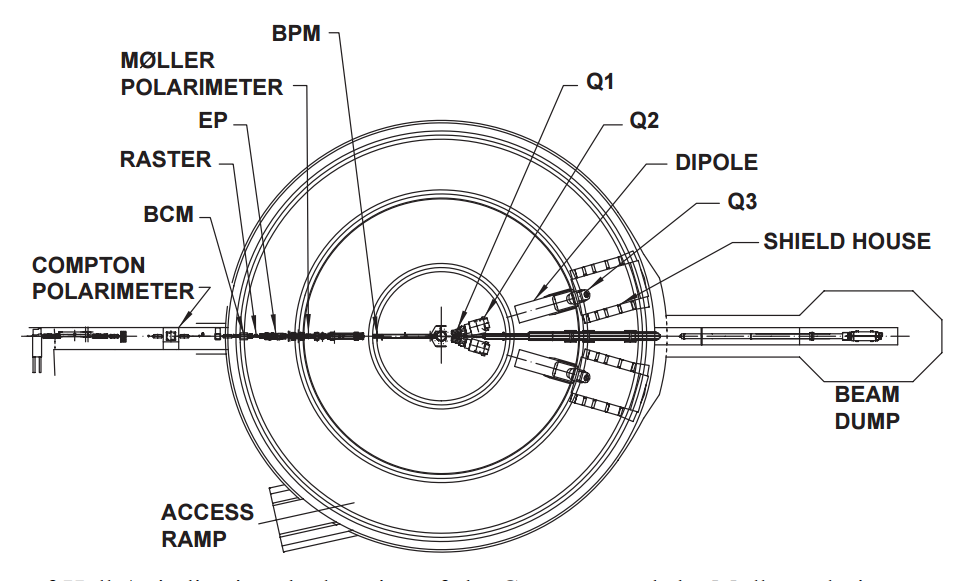
\includegraphics[width=14cm]{BeamLine.png} 
	 	 \end{figure} 	
	 	 	
	 \paragraph{} The main beam line components of the BPMs consist of four open-ended antennas. Figure \ref{BPMimg} shows a BPM chamber and figure \ref{BPM_4} shows the layout of the four antennas as you look down the beam line. In this chamber, the design of three of the four antennas can be seen. The antennas are titled $u_+$, $u_-$ and $v_+$, $v_-$. The antennas receive an induced signal as electrons pass to determine the beam position in the u and v directions. The direction of the beam is determined by using the two BPMs in conjunction with timing information provided. The accuracy of the BPMs requires an absolute measurement of the electron beam's position to calibrate the BPMs and a internal input oscillation measurement names twiddle to supply BPM signal coefficients.  \cite{BPM,BPM2}.
	 	 	\begin{figure}[H]
	 	 		\centering
	 	 		\caption{BPM design diagram, from JLab instrumentation	group. Beam direction is from left to right \cite{BPM2}. }
	 	 		\label{BPMimg}
	 	 		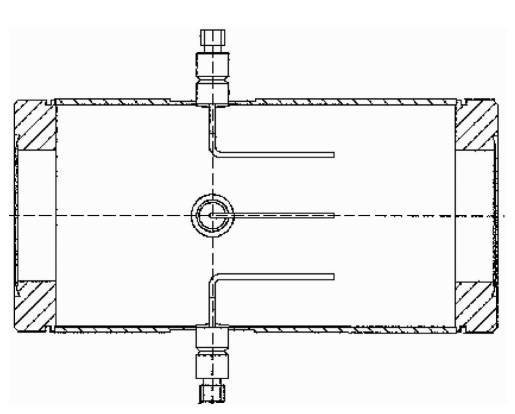
\includegraphics[width=10cm]{BPM.png} 
	 	 	\end{figure} 	
	 
	 		\begin{figure}[H]
	 			\centering
	 			\caption{BPM design diagram, looking down the beam line\cite{BPM2}. }
	 			\label{BPM_4}
	 			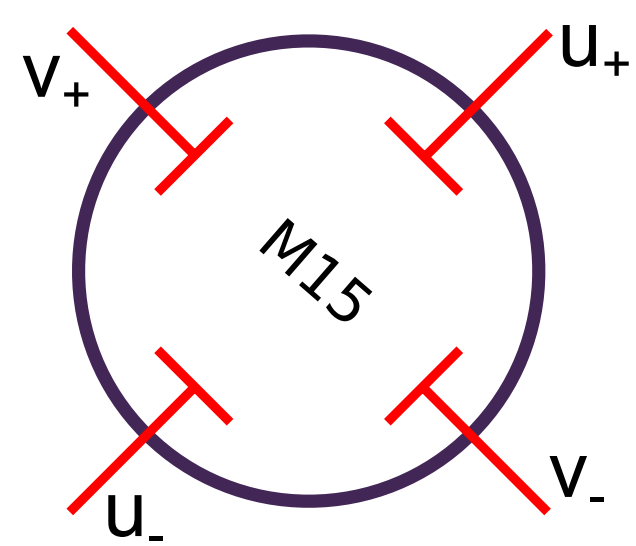
\includegraphics[width=10cm]{BPM_4.png} 
	 		\end{figure} 

	
	 \paragraph{} Damage to a target system from intense beam can cause extreme fluctuations in the target's temperature and density. A raster was used to counteract the damage caused by a focused beam. The raster used two magnetic fields produced by two dipoles to spread the electron beam out. This produces a large rectangle interaction area on the front face of the target container. A triangle wave of 25 kHz was used to control the coils of the dipole magnets. The raster systems are located $\approx$17 meters before the target chamber (upstream of the target\cite{BPM2}). The rasters position can be seen in figure \ref{HallA}. Safety constraints administrated by the target group at JLAB limited the minimum size of the raster spot for the MARATHON experiment to two millimeters by two millimeters. This limit was installed has a safety concern for the tritium target. 
	 \paragraph{} The Hall A raster system consists of four dipoles. Two dipoles produce magnetic fields in the horizontal direction of the lab frame and two in the vertical. The upstream raster and downstream rasters include one vertical and one horizontal dipole. The relative change in position of the incoming electrons are controlled by the current supplied to the dipoles. In order to obtain the change in beam position due to the rasters, a calibration between the raster current and measured beam position were obtained.  
	 
	 \paragraph{}The electron beam energy is located in many of the equations used in an electron scattering experiment. This can cause a noticeable increase in systematic error if the beam energy measurement is not made precisely. At JLAB for the MARATHON experiment, the beam energy was measured in two ways. In Hall A, the beam energy was measured by using the (e,e$\prime$p) method. On the beam line, 17 meters upstream from the target an ep scattering chamber is located. The beam was directed into the target containing a rotating 10-30 $\mu$m thick tape of C$H_2$. The scattering angle of the electron and the recoil angle of the proton are used to determine the beam energy using equation \ref{EP}. Where $M_p$ is the mass of the proton and $\theta_p, \theta_e$ are the scattered angle of the proton, electron respectively. 
	\begin{equation}
	\label{EP}
	E = Mp \frac{cos\theta_e + \frac{sin\theta_e}{tan\theta_p}-1}{1 - cos\theta_e} 
	\end{equation}
	The beam energy was also measured using the ark measurement method \cite{Flay}. This method uses changes is beam position and precise measurements of the magnetic fields around the beam line to determine the energy of the electron beam. The angle at which the electrons are bent through is related to the momentum of the electrons,
	\begin{equation}
	\label{arc}
	p = k \frac{\int \vec{B} \cdot d\vec{l}}{\theta}.
	\end{equation}	
	In equation \ref{arc}, p is the momentum of the electrons, $\theta$ is the bend angle, and $\vec{B}$ is the magnetic field the electron experiences. Then using the momentum of the electron, the energy of the beam can be extracted. The error on the beam energy measurement is $\delta$ E/E $\approx$ 2 $* 10^{-4} $ \cite{EPMet, Flay}.  The MARATHON experiment used both methods to accurately determine the electron beam energy.
	
		  	\begin{figure}[H]
		  	 	 		\centering
		  	 	 		\caption{Hall A Current Monitor components \cite{BCM1}. }
		  	 	 		\label{BCMpng}
		  	 	 		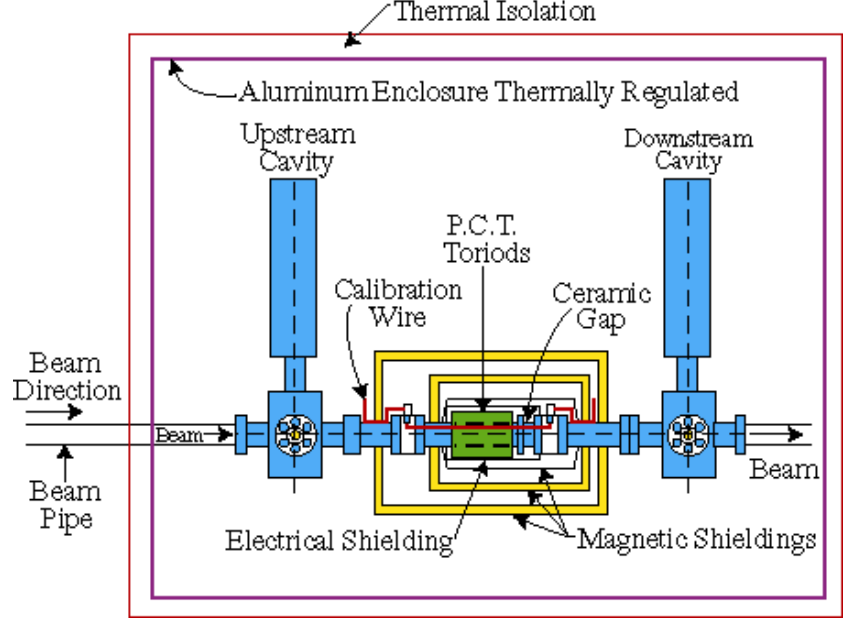
\includegraphics[width=10cm]{BCM1.png} 
		  	\end{figure}
	
	\paragraph{} The main process of measuring the scattering yield for a calculation of a cross section looks at finding the ratio of the number of electrons scattered to the number of electrons sent. In order to accurately determine the number of electrons sent to scatter with our target system, Hall A use a highly accurate and non-invasive beam current monitor(BCM). The Hall A BCM has an a4bsolute accuracy of 0.2 percent as long as the current is between 1 and 180 $\mu$A. The BCM used in Hall A consists of three main components: a Parametric Current Transformer (PCT) and two pill box cavities. Figure \ref{BCMpng} shows the components in the Hall A BCM.  The BCM produces an RF signal that is proportional to the beam current. An 10 kHz down converter, RMS-to-DC converter, voltage-to-Frequency converter, and a scaler are used to inject the current signal into the Hall A DAQ. Proportionality constants are determined in the calibration process to correctly integrate the charge for a given amount of beam current\cite{BCM1}. Continue after the initial beam line components, an electron will enter into the target chamber, housing the target system.
	  
\section{Target}
\paragraph{} The Hall A Tritium Target(HATT) system was used for the Tritium run group of experiments. The HATT target chamber was repurposed from a previously used cryo-target chamber in order to reduce the financial cost of designing a new target chamber. The refurbishing of the cryo-target chamber consisted of adding in new safety features to prevent and mitigate a tritium leak.  A 4 inch long collimator with an inner diameter of 0.4 inch was added inside of the target chamber but upstream of the target ladder to prevent the beam from striking the thin side wall of the aluminum cell. In case of a tritium leak in the target chamber, an exhaust system was installed to control the amount of tritium exposed to the Hall.\cite{HATT_eng}  Figure \ref{HATT} shows the HATT system with the target ladder in the home position and the scattering windows removed. 
\begin{figure}
	\caption{Target Images}
	\subfloat[A image of the HATT. \cite{DHimages}]{{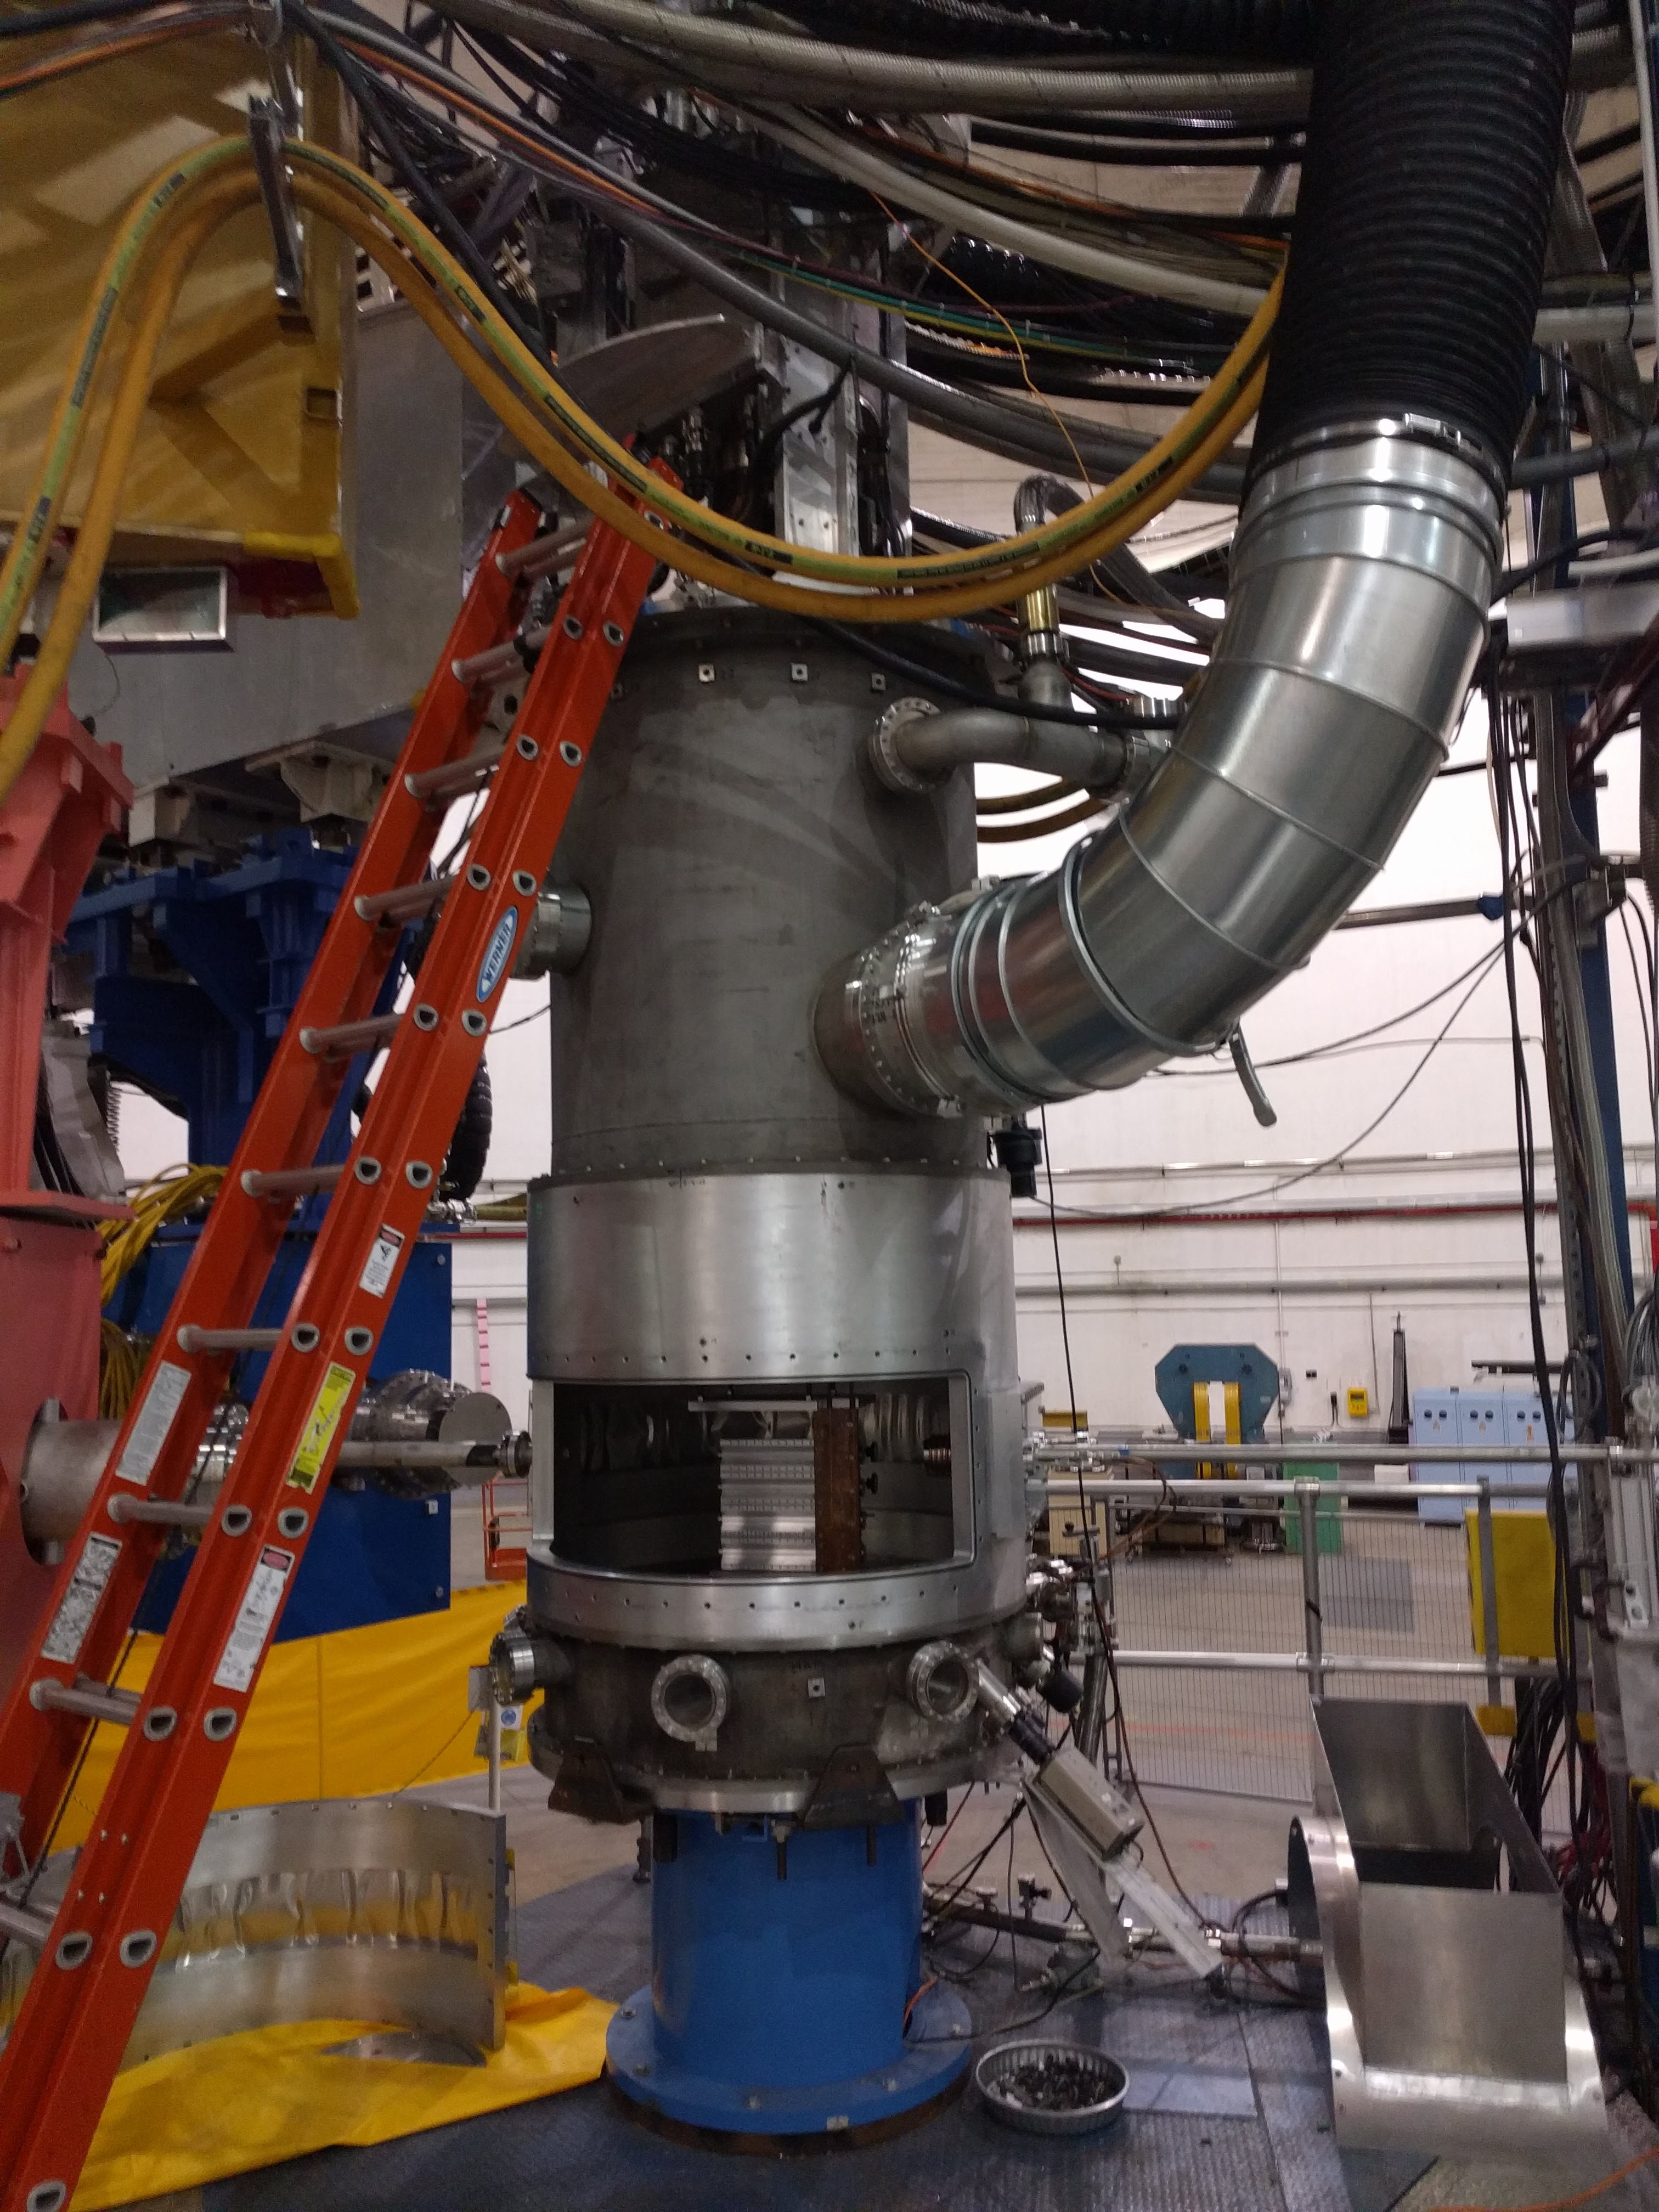
\includegraphics[width=6cm]{HATT.jpg} }}
	\quad
	\subfloat[Image of the Hall A Tritium Target Ladder. \cite{DHimages}]{{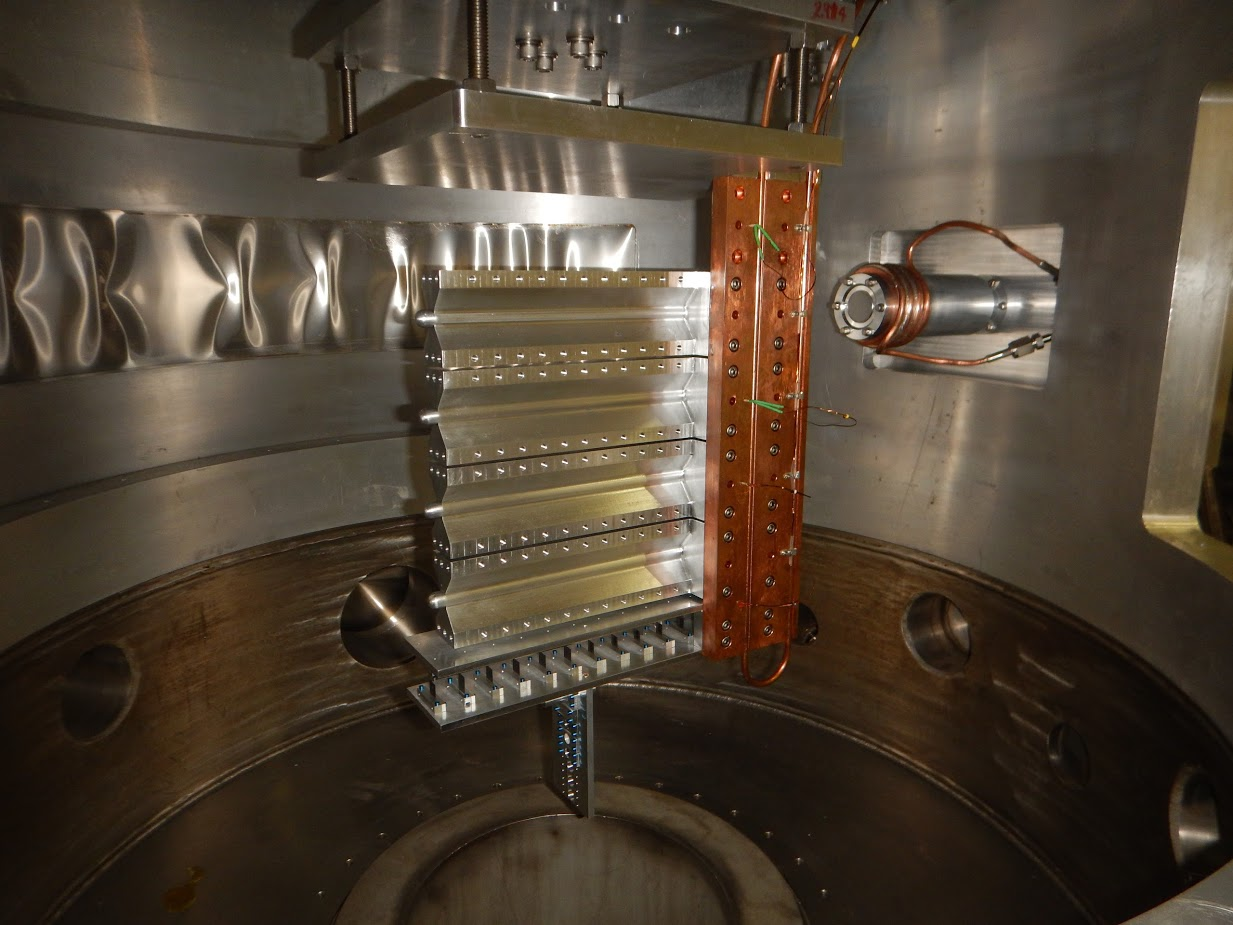
\includegraphics[width=12cm]{HATT_Ladder.JPG} }}
	\label{HATT}


\end{figure}
A picture of the HATT ladder installed in the HATT system is shown if figure \ref{HATT}. The ladder contains both gaseous cells and solid targets. The MARATHON experiment had five gas cells. The top four of the gas cells were filled with tritium, deuterium, hydrogen, and $^3$helium, from top to bottom respectively. Due to safety restricts the tritium cell was not installed until the HATT system could be closed. The bottom most cell was left empty, to complete end cap subtractions. The lower half of the target ladder contains the solid targets used during the MARATHON experiment. Listed from top to bottom, the solid targets used were a pair of thick aluminum foils, carbon multifoil, single carbon foil, and a carbon foil with a 2mm diameter hole. The thick Al foils were used to aid the target window background subtraction. The multifoil target also know has the optics target was used to calibrate the z-axis  reconstruction of the optics matrix. The single carbon foil and carbon hole were used to calibrate the BPMs and rasters and to determine the off set of the central line of the detector. 



\section{High Resolution Spectrometers}
Electrons that successfully scatter from the target may end up in either of the two HRSs(High Resolution Spectrometers). The HRSs were designed to detect charged particles with a high degree of precision. 
In order to achieve a high level of resolution in momentum and angle, the HRSs were designed with a magnet configuration of QQ$D_n$Q (quadrupole, quadrupole, dipole, and quadrupole). The vertical bending dipole provides the field required to transport the scattered particles through the 45$^\circ$ bending angle to the detector hut. A drawing of an HRS can be seen in figure \ref{hrsfull}. The first quadrupole(Q1) focuses the incoming electrons in the vertical plane. The following two quadrupoles (Q2 and Q3 provide transverse focusing. This optical design allows the use of extended gas targets with no substantial loss in solid angle\cite{HallA}.  The spectrometers were designed to perform various functions which include: triggering the data acquisition system (DAQ) when certain requirements are met, gathering the position and direction of individual particles to reconstruct a track, provide precise timing information for time of flight calculations, and identify many different particle types that pass through the detector system. In order for both the Left HRS (LHRS) and Right HRS (RHRS) to  complete the required task, they contain a myriad of detectors. The HRSs use drift chambers, scintillators, cerenkov detectors, and shower calorimeters. Both the Left and Right HRSs contain two planes of scintillators to function has the main trigger for the detector package. The vertical drift chambers (VDC) that lay at the front of the detector in conjunction with the Shower that lies in the back of the detector provide information for reconstructing the particle tracks and precise timing. Particles are identified by the cerenkov, shower calorimeters, and pion rejectors that are contained in the left or right HRS. The layout of the individual detectors that make up the left and right detector package are shown in figure \ref{hrsss}  \cite{HallA}.

\begin{figure}
	\centering
	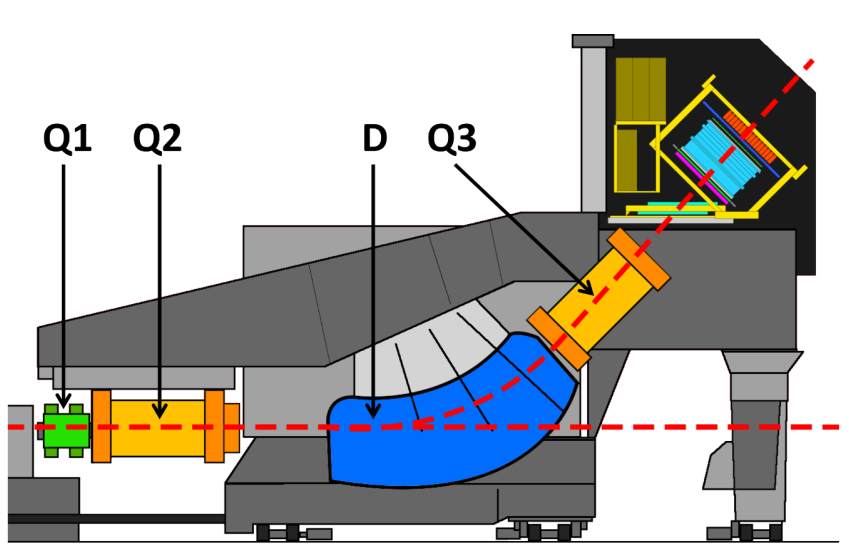
\includegraphics[width=10cm]{HRS_full.png}
	\caption{A side view of a HRS \cite{HallA}.
	\label{hrsfull}}
\end{figure}

\begin{figure}
	\centering
	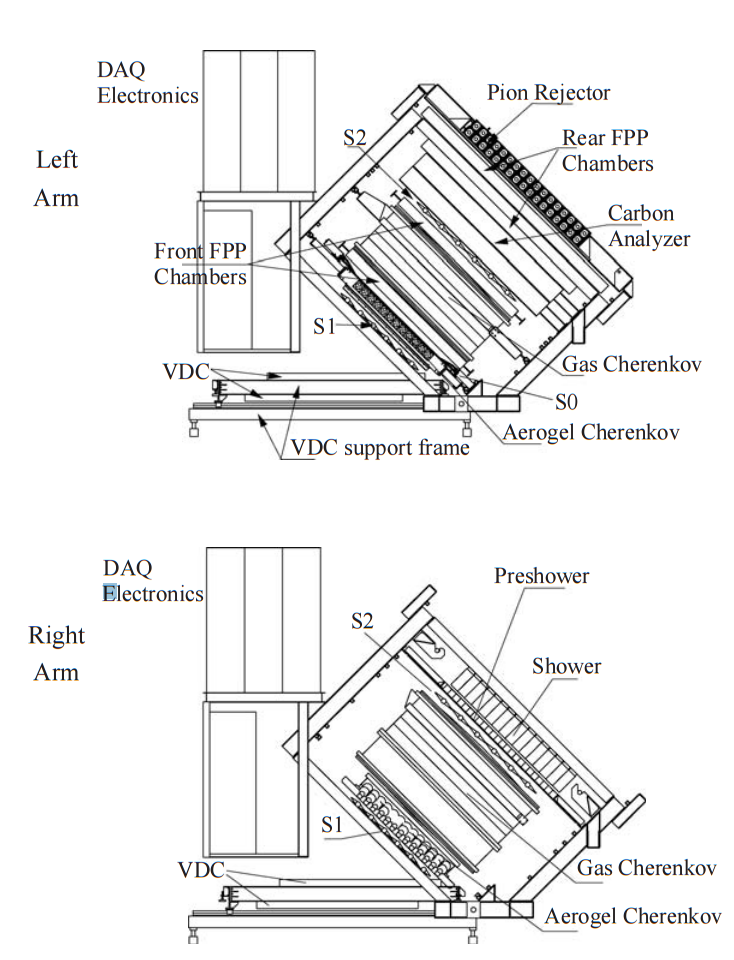
\includegraphics[width=10cm]{HRSs.png}
	\caption{A view of both the left(top) and right(bottom) detector stacks inside the left and right HRS \cite{HallA}.
	\label{hrsss}}
\end{figure}

	\subsection{Vertical Drift Chambers}
	Each of the spectrometers housed in Hall A contains a vertical drift chamber(VDC). Each VDC contains two planes of crossing sense wires. Shown in figure \ref{VDC_profile}, the two planes of the VDC lie a distance of 0.335m apart \cite{drift}. The lower plane of the VDC is positioned at the approximate focal plane of the HRS and lies in the horizontal plane of the Hall A coordinate system. The sense wires located in the VDCs cross orthogonally. They are offset by $45^\circ$ in respect to the dispersive and non-dispersive directions. 
	
	\cite{drift}
	
	
	\begin{figure}
	\centering
	
	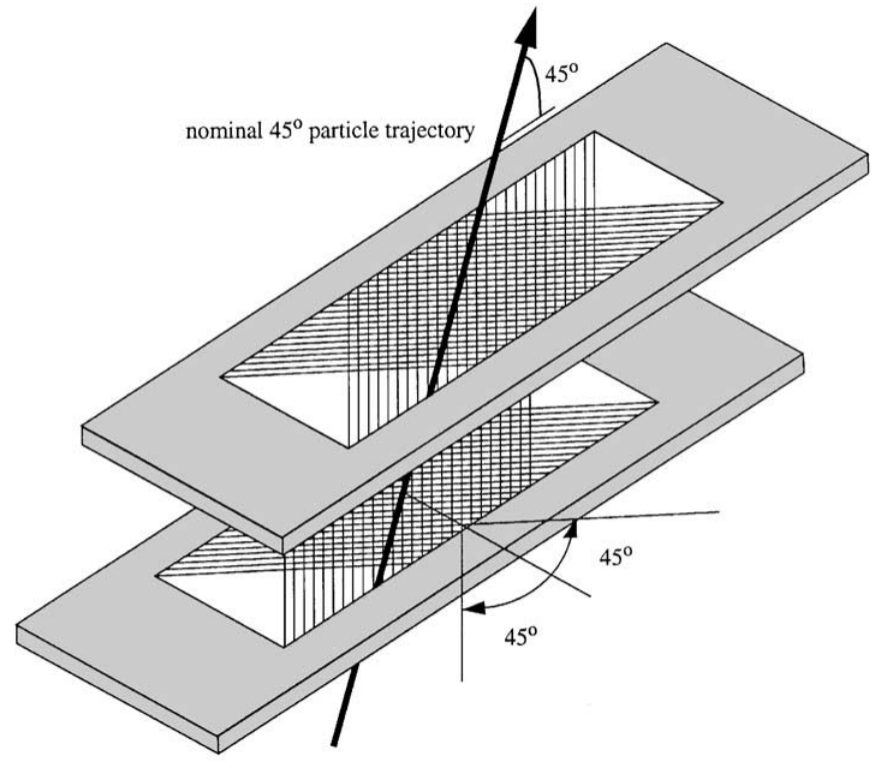
\includegraphics[width=10cm]{VDC_profile_view.png}
	
	\caption{A sketch of the two VDC planes in the HRSs with a particle traveling through the detector at 45$^\circ$.\cite{drift}.
	\label{VDC_profile}}
	\end{figure}
	
	
	
	
	
	\subsection{Scintillators}	\subsection{Cherenkov}
	\subsection{Shower Calorimeter}
	\subsection{Pion Rejector}
	\subsection{FPP Chambers}

\section{Trigger Setup}
	\begin{figure}
	\centering
	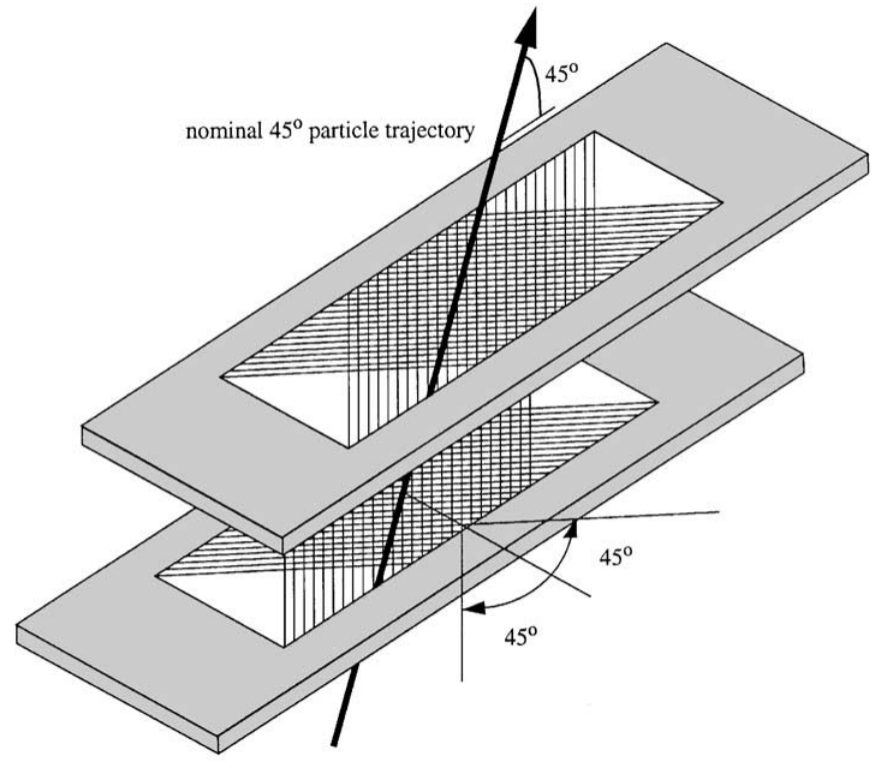
\includegraphics[width=10cm]{VDC_profile_view.png}
	\caption{A sketch of the two VDC planes in the HRSs with a particle traveling through the detector at 45$^\circ$.\cite{drift}.
	\label{trigger_Setup}}
\end{figure}



\section{DAQ - Data Acquisition System}

\section{Kinematic Settings}










   		%
\chapter{Calibration}





\paragraph{}The information provided by the detectors originate through small changes in current and voltage sent through the DAQ electronics. These signals are transformed into useful information through calibration constants. The beam line elements and the individual detector components were calibrate to supply highly precise and accurate data. 


\section{Beam Line}
 \paragraph{} The BPM signal coefficients are determined by a twiddle measurement. An RF module attached to the BPM antennas is used to pass a signal out of each of the antennas, one at a time. This will allow the determination of the conversion factor for the BPM signal to relative beam position. Two harps were used to provide the absolute measurement required for calibrating the BPMs. Figure \ref{harp} contains a drawing of the harps used in Hall A. The harps were moved into the beam line when calibration data is needed, but must be moved out for the production of experimental data because the harp wires are intrusive to the beam operation.  The harp forks are aligned perpendicular to the beam line, to allow the harps to be moved in and out of the beam line. Three different wires are used to determine the horizontal and vertical position of the beam. Each wire has one of three orientations: vertical, sloped down or sloped up. The two sloped wires are angled at 45$^{\circ}$ relative to the wire frame. As the harp fork is moved into the beam, the wires receive a signal as the beam interacts with the wires. The two sloped wires are used together to determine the vertical position of the beam. The vertical wire is used to determine the horizontal position of the beam \cite{BPM,BPM2}. 
		 	\begin{figure}[H]
		 		\centering
		 		\caption{A schematic layout of a harp fork \cite{BPM2} }
		 		\label{harp}
		 		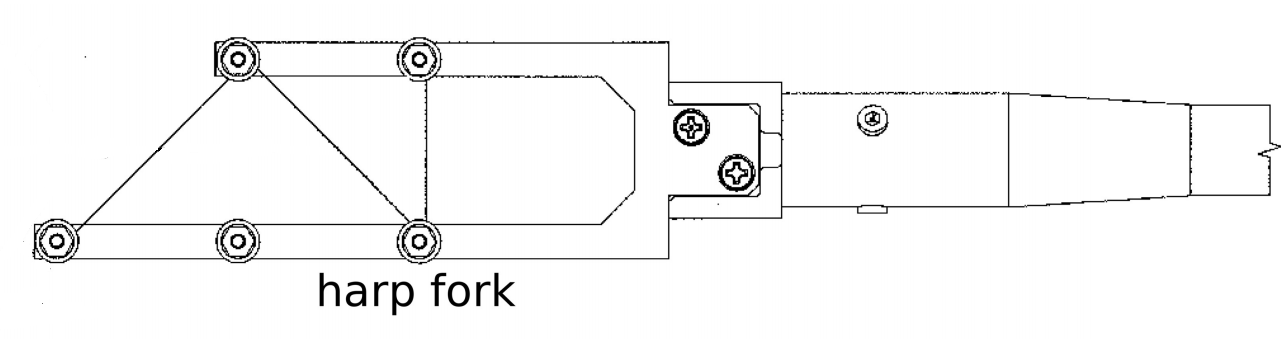
\includegraphics[width=14cm]{harp.png} 
		 	\end{figure}  	
	 
	 \paragraph{}The location of the wires on the harp frame and the position of the harp fork were used to calculate the absolute beam position. The BPM calibration coefficients were determine by using a bulls eye scan, figure \ref{bulls} shows an example of the five positions used to calculate the BPM calibration coefficients. The harp scan results are substituted into equation \ref{BPM_eq} for the X and Y positions. Using all five points and an $R^2$ regression technique, the coefficients can be determined with great accuracy. These highly accurate BPMs were crucial in reducing systematic error in the final results obtained from this experiment. 
	 \begin{equation}
	 \label{BPM_eq}
	 \begin{pmatrix}
	 X_{position}\\
	 Y_{position}
	 \end{pmatrix}
	=
		 \begin{pmatrix}
		 C(0,0) & C(0,1)\\
 		 C(0,0) & C(0,1)\\
		 \end{pmatrix}
		 *
		 	 \begin{pmatrix}
		 	 X_{BPM}\\
		 	 Y_{BPM}
		 	 \end{pmatrix}
		 	 +
		 	 \begin{pmatrix}
		 	 X_{offset}\\
		 	 Y_{offset}
		 	 \end{pmatrix}			 
	 	 \end{equation}
	
		\begin{figure}[H]
			\centering
			\caption{The X and Y position for a Bulls eye scan for BPM calibration. }
			\label{bulls}
			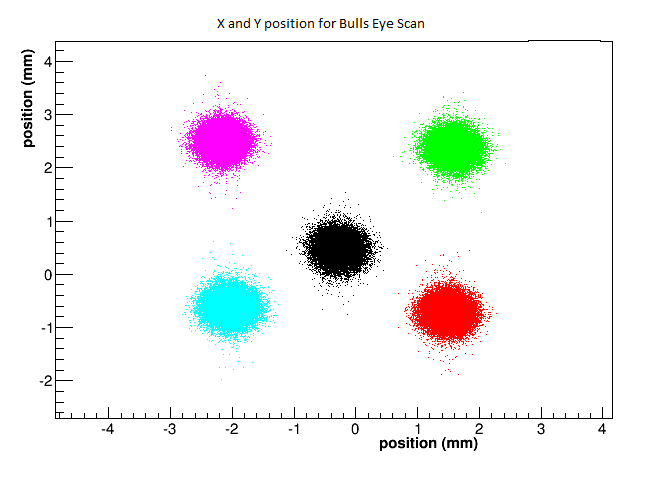
\includegraphics[width=10cm]{bulls.png} 
		\end{figure} 	
	
    	\chapter{Data Analysis}
\paragraph{}The goal for the MARATHON experiment is to determine the EMC effect for the two A=3 systems $^3$He and $^3$H, extract the  $F_2^n$/$F_2^p$, and calculate the $d$/$u$ quark distribution ratios. The goal of this analysis is to determine the EMC effect for the two A=3 systems via the ratio of measured cross sections. The cross-section of a scattering interaction is the probability of that event happening. In order to measure the probability of an event happening, a ratio has to be calculated between the magnitude of the number of those events versus the number of times that event could of happened. This analysis will use data from the HRSs, beam line detectors, and target information to measure the cross-section of $^3$He and $^3$H for kinematics of 0.2 $< x <$ 0.82. 
\section{Analysis Software}
\paragraph{}Hall A at JLab uses an analysis software (Analyzer) that is built on top of ROOT. The Analyzer is used to decode raw data received from TDCs, ADCs, and scalars into meaningful results. The decoding process uses raw data from the detectors in the HRSs and on the beam line to create an event. This event is assigned a track if applicable, and the events signal from the detectors are stored into a ROOT file. This ROOT file contains the raw and calibrated detector data from each signal, the track information, and physics variables calculated via the calibrated data and track information. 
\subsection{Tracking}
\paragraph{}The Analyzer uses calibrated VDC data to calculate the track of an event. The detector calibration was discussed in chapter \ref{ch:ExpUp}. The event tracking is used to determine the scattered angle and momentum of the electrons detected. The track determined from the VDCs is in reference to the detector coordinate system. The Analyzer uses a optics matrix to relate the tracking information between all coordinate systems used in the Hall A analysis process. The coordinate systems will be briefly discussed in this section. A more complete guide with in-depth discussion of the coordinate systems is discussed in \cite{espace}. The coordinate system definitions and relations are obtained from \cite{espace,optics,HallA}.
\begin{itemize}
	\item \textbf{Hall Coordinate System(HCS):} The intersection of the electron beam and the vertical symmetry axis of the target system defines the origin of the HCS. This allows for $\hat{z}$ to point along the beam line towards the beam dump and $\hat{y}$ is up. 
	\item \textbf{Target Coordinate System (TCS):} The TCS is unique to the individual HRS. The $\hat{z}$ axis of the TCS is defined by a line perpendicular to the surface of the spectrometers sieve slit aligned with the midpoint of the center hole. $z_{tg}$ points away from the target towards the spectrometer. Nilange Liyange states in reference \cite{optics}, "In the ideal case where the spectrometer is pointing directly at the hall center and the sieve slit is perfectly centered on the spectrometer, the z$_{tg}$ axis passes through the hall center." Using the idea case, the origin of the TCS is defined by a set distance from the sieve surface. For the Left HRS, the TCS origin is 1.181m from the sieve, and for the Right HRS it is 1.178m. In the ideal case, the TCS origin is the HCS origin. Figure \ref{fig:TCS} shows the TCS with a an electron scattering event from a foil.  
	\begin{figure}[]
		\centering
		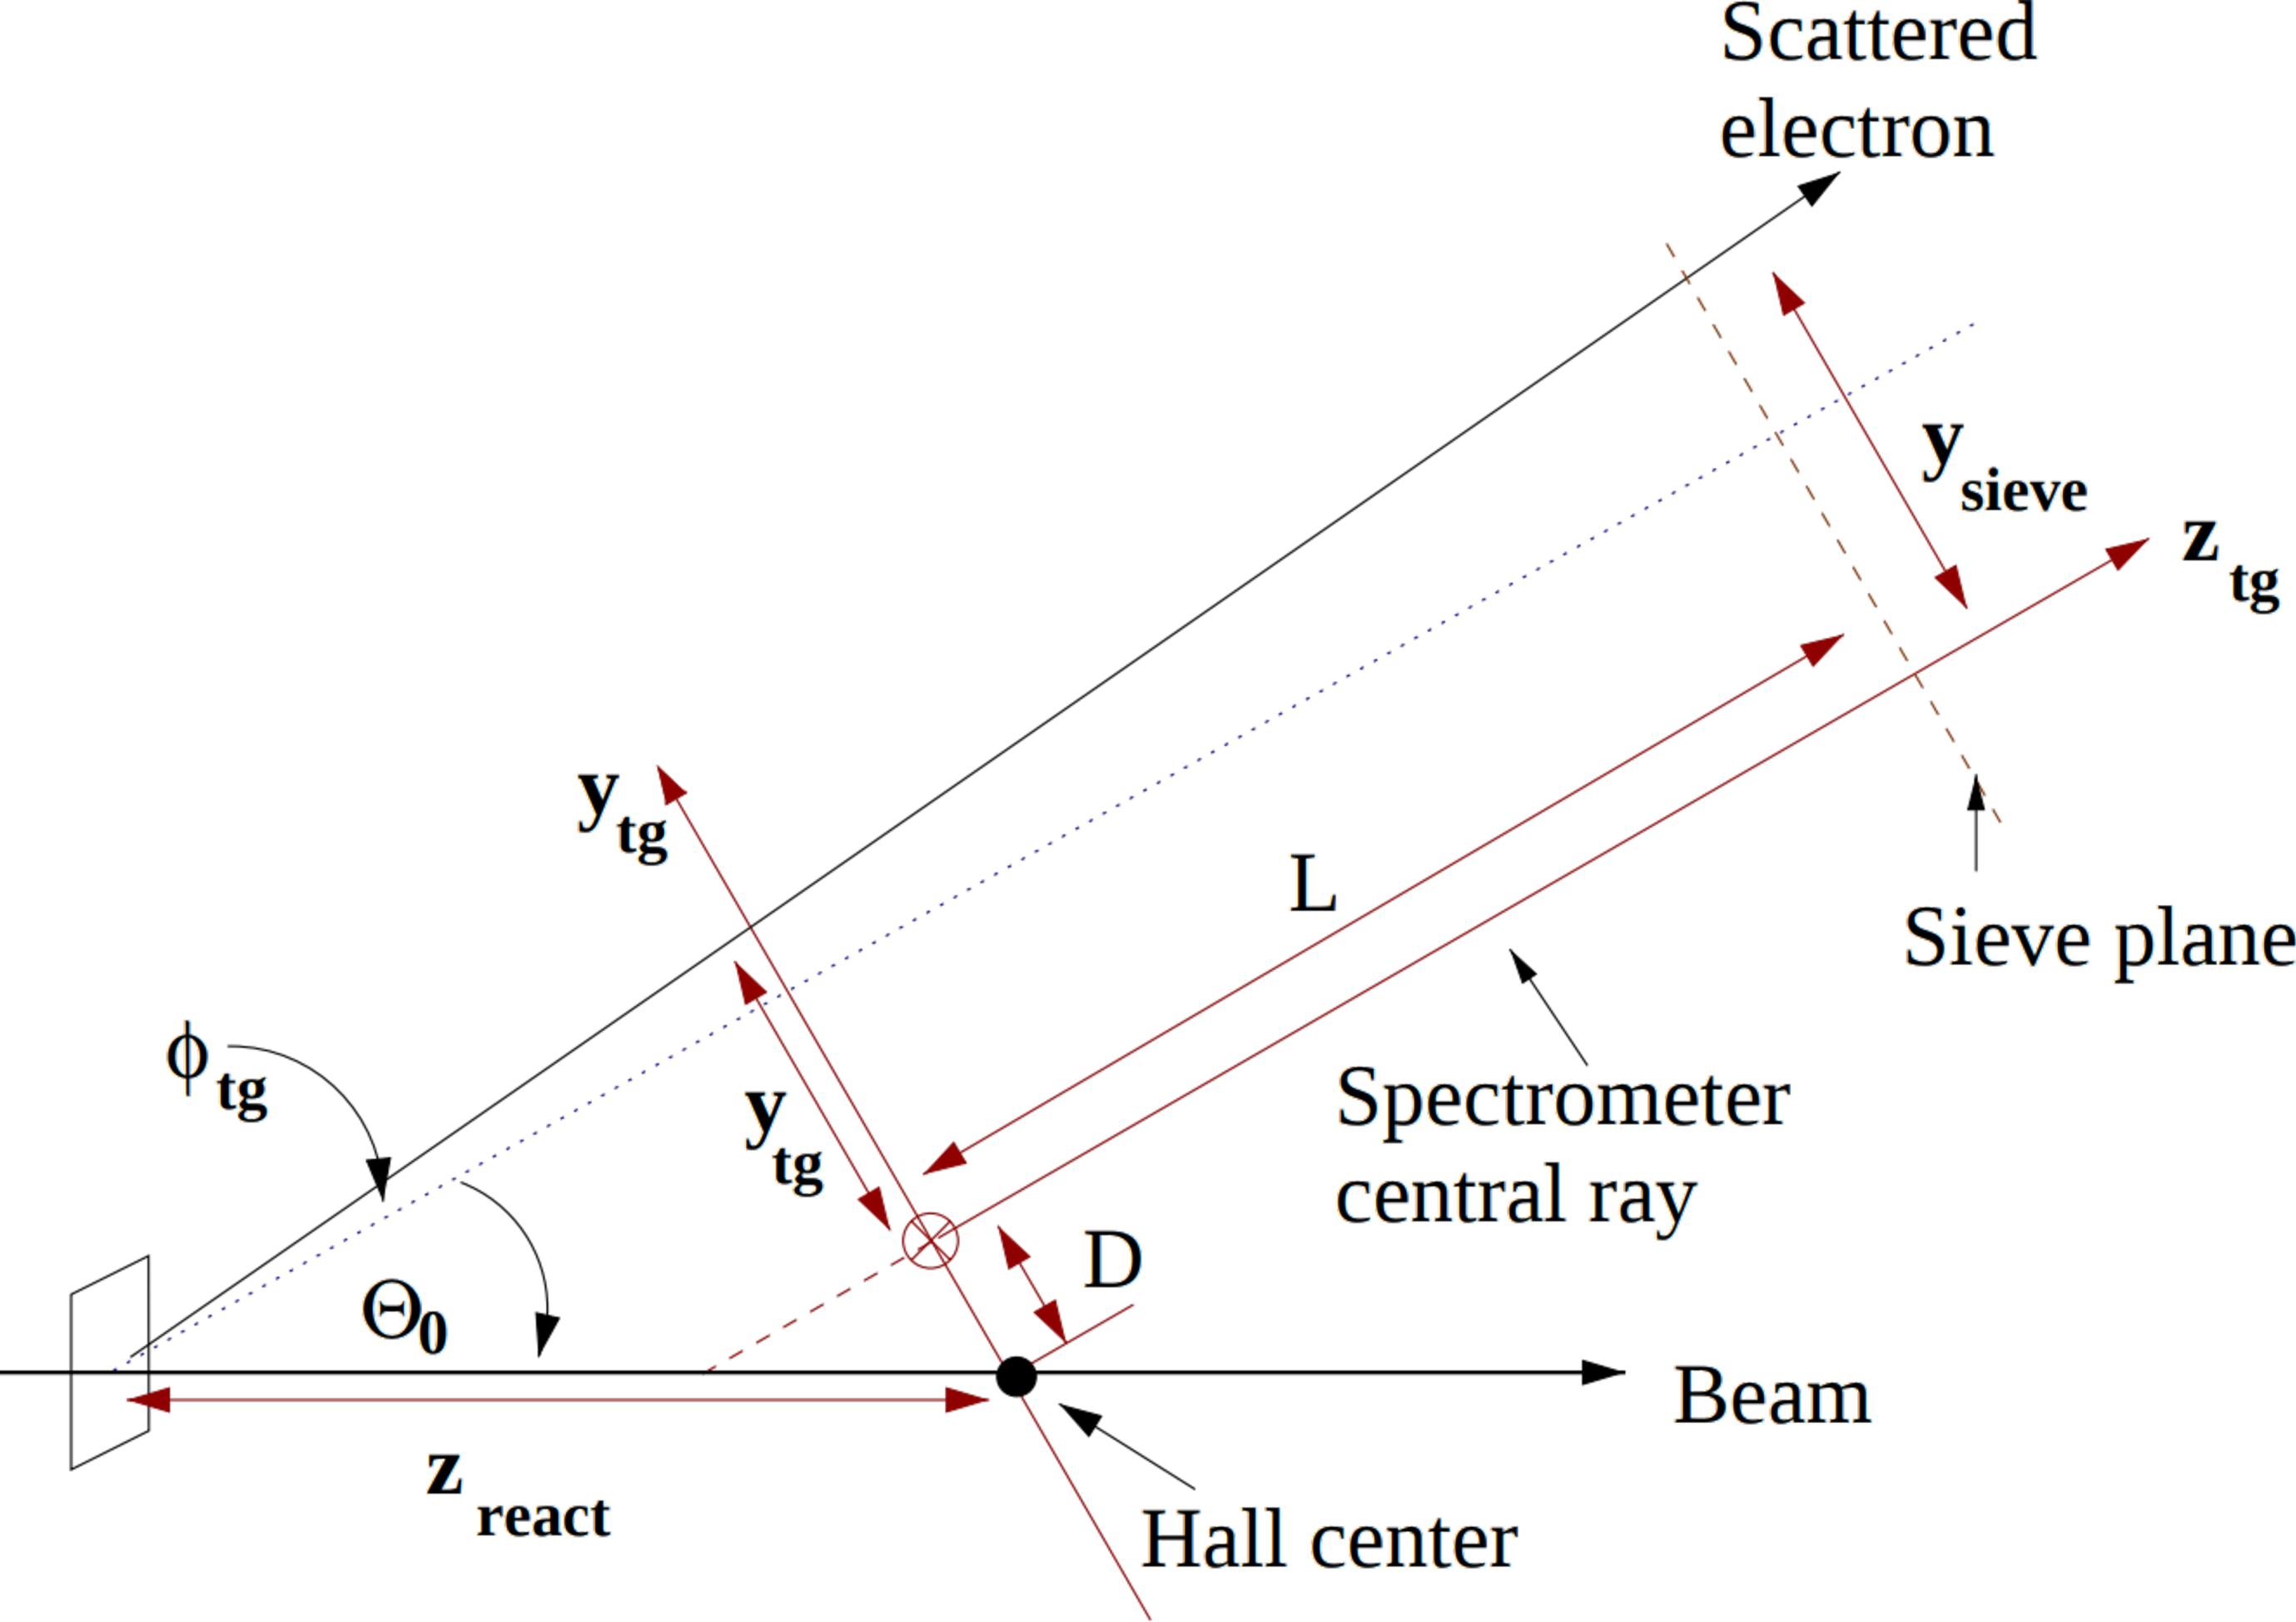
\includegraphics[width=11cm]{TCS.pdf}
		\caption{The TCS for an electron scattering event as seen from above. The event happens at $z_{react}$ distance from the Hall center. \textbf{L} is the distance from the Hall center to the sieve plane. \textbf{D} is the horizontal displacement of the spectrometer axis from the ideal position. $\Theta$ is the spectrometer's central angle \cite{optics}. }
		\label{fig:TCS}
	\end{figure}
	\item \textbf{Detector Coordinate System (DCS):}  The origin of the DCS is at the intersection of wire 184 of the U1 and V1 planes of the first VDC. "$\hat{y}$ is parallel to the short symmetry axis of the lower VDC \cite{espace}." $\hat{z}$ is vertically up, perpendicular to the vdc planes.  $\hat{x}$  points away from the center of curvature of the dipole. The DCS values are calculated by using the intersection points of the 4 VDC planes and the spacial information of the VDC planes.
	\item \textbf{Transport Coordinate System (TRCS) at the focal plane:} Rotating the DCS clockwise around its y-axis by 45$^\circ$ generates the TRCS. The TRCS can be expressed by  DCS variables. 	
	\item \textbf{Focal Plane Coordinate System (FCS):} The FCS is used to transport an event's track from the DCS to the TCS. The FCS is determined by rotating the DCS around its y-axis by the angle between the local central ray and the $\hat{z}$ axis of the DCS. The local central ray is defined as a ray with $\theta = \phi =0$ for the corresponding relative momentum $\frac{\Delta_p}{p}$ \cite{optics}. In the calculation of the FCS, the offsets of the VDCs are used to correct any misalignments.  
\end{itemize}
\paragraph{} The Analyzer provides two spatial coordinates and two angular coordinates for each event. These coordinates are determined by data received via the VDCs and decoded into the DCS. $x_{det}$ and $\theta_{det}$ is the particle's position and tangent of the angle made by its trajectory along the dispersive direction. $y_{det}$ and $\phi_{det}$ is the particle position and tangent of the angle perpendicular to the dispersive direction \cite{optics}. Using rotation matrices and other transfer definitions these DCS coordinates are converted to the FCS. The analyzer uses a calibration matrix to transport the FCS to the TCS. The first order approximation of the matrix can be defined as:
\begin{equation}
\begin{bmatrix}
	\delta \\
	\theta \\
	y      \\
	\phi   
\end{bmatrix}_{tg}
=
\begin{bmatrix}
	\langle \delta \vert x \rangle &\langle \delta \vert \theta \rangle & 0 & 0\\
	\langle \theta \vert x \rangle &\langle \theta \vert \theta \rangle & 0 & 0\\
	0 & 0 & \langle y \vert y \rangle &\langle y \vert \phi \rangle\\
	0 & 0 & \phi y \vert y \rangle &\langle \phi \vert \phi \rangle
\end{bmatrix}
\begin{bmatrix}
	x     \\    
	\theta \\
	y      \\
	\phi   
\end{bmatrix}_{fp}.
\end{equation}
The relationship between the focal plane variables and the target coordinates our conventionally expressed in a set of tensors, defined as Y$_{jkl}$, T$_{jkl}$, P$_{jkl}$, and D$_{jkl}$. These tensors are polynomials in x$_{fp}$ and are optimized to the 5th order. They can be use to relate the FCS to the TCS by the following relations:
\begin{align}
y_{tg} &= \sum_{j,k,l} Y_{jkl}\theta^j_{fp}y^k_{fp}\phi^l_{fp} \\
\theta_{tg} &= \sum_{j,k,l} T_{jkl}\theta^j_{fp}y^k_{fp}\phi^l_{fp} \\
\phi_{tg} &= \sum_{j,k,l} P_{jkl}\theta^j_{fp}y^k_{fp}\phi^l_{fp}  \\
\delta_{tg} &= \sum_{j,k,l} D_{jkl}\theta^j_{fp}y^k_{fp}\phi^l_{fp} 
\end{align}
The elements of the optics matrix used for the transporting from the FCS to the TCS are part of the tensors,Y$_{jkl}$, T$_{jkl}$, P$_{jkl}$, and D$_{jkl}$. The elements of the optics matrix are calculated via an optics calibration using a sieve slit and multi foil optics target. The procedure for calculating those matrix elements is in reference \cite{optics}. 
\paragraph{}Along with the tracking information in the TCS, the analyzer also provides the location of the reaction vertex, the scattering angle for the electron event, and the momentum of the scatted electron from the tracking information. The reaction vertex along the beam line, z$_{react}$, is the location where the scattering event happened in the HCS. z$_{react}$ can be found via the following relationship:
\begin{equation}
z_{react} = \frac{-(y_{tg} + \text{Spect\_Offset}_y) + x_{beam}(cos(\Theta_0) - \phi_{tg}sin(\Theta_0))} {cos(\Theta_0)\phi_{tg} + sin(\Theta_0)}
\end{equation}
The relationship for z$_{react}$ includes terms for the offset due to the mis-pointing of the spectrometer (Spect\_Offset$_y$), the offset of the beam at the point of intersection with the target (x$_{beam}$), and the setting for the spectrometer central angle ($\Theta_0$). The scattering angle of the electron, $\theta_{scat}$, is determined by a relationship wit the TCS angle coordinates $\theta_{tg}$ and $\phi_{tg}$ and the angle setting of the spectrometer. The relationship used to calculate the scattering angle from the target coordinates is described in reference \cite{HallA}, as:
\begin{equation}
\theta_{scat} = arccos \left( \frac{cos(\theta_{0})- \phi_{tg}sin(\theta_{0})} {\sqrt{1 + \theta_{tg}^2 + \phi_{tg}^2}} \right) \label{scatangle}
\end{equation}
The accuracy of the TCS angles $\theta_{tg}$ and $\phi_{tg}$ determine the accuracy of the measured scattered angle. The precise measurement of the scattering angle is crucial to every electron counting experiment. In order to provide accurate measurement of the scattering angle, a set of measurement surveys are completed. These surveys measure the:
\begin{itemize}
	\item the target position,
	\item the spectrometer central angle,
	\item the mispointing of the spectrometer nominal central ray from the hall center,
	\item the position of the sieve-slit center with respect to the nominal central ray,
	\item the position of the BPMs with respect to the ideal beam line \cite{HallA}.
\end{itemize} 
The results from the surveys have an approximate systematic uncertainty of 0.5 mm due to equipment uncertainties. The contribution of all the measurements uncertainties added in quadrature provide an approximate 0.6 mrad uncertainty to the overall measurement of the scattered angle \cite{HallA}. 
\paragraph{}The momentum of the scatted electron is also calculated via tracking information.  $\delta_{tg}$, the relative momentum of an event, is used in the calculation of the momentum of a particle traveling through the spectrometer. $p$, the absolute momentum for an event, is determine through the following relation.
\begin{equation}
p = p_0(1+\delta_{tg})
\end{equation}
 
\section{Electron Counting}
\paragraph{}

%cuts, total electrons per kinematic, binning in x 

\section{Efficiencies}
\paragraph{}The high resolution spectrometers are capable of detecting a myriad of particles that track through the detectors. The design of an experimental trigger uses the properties of the individual detectors to capture data of meaningful events. Many accidentals, background, and unwanted events trigger the data acquisition system, and some good electrons are missed by our DAQ. The removal of these unwanted events takes place during analysis via software cuts. Restricting the applicable signal from certain detectors through different cuts allows for the rejection of background particles and prevents contamination in the yield extraction. 

\subsection{Computer and electronic Lifetime}
\paragraph{}The signal from events that fire the DAQ travel through electronics like amplifiers and logic modules on its way to be recorded by the TDCs and ADCs. The processing of these signals require time at each stage. During that time another event will be discarded due to limitations in the hardware. This time when the DAQ system cannot handle another event is known as the dead-time of the system. Lifetime therefor is the percentage of time when an event can be recorded. The lost events need to be account for during the analysis process. The lifetime of the DAQ system for the MARATHON experiment was measured by determining the percentage of events that were recorded relative to the number of events that fired the corresponding trigger. The lifetime for the MARATHON experiment depended on the rate of events. The lifetime during the highest rate kinematic was determine to be 0.947, and climbs to 0.998 for the highest angle setting. Listed in table \ref{LTtable} are the calculated values for lifetime at each kinematic. 

\begin{table}[]
	\textbf{Livetime for each kinematic }\par\medskip
	\begin{tabular}{|l|l|l|l|l|l|l|l|l|l|l|}
		\hline
		Kin      & 1 & 2 & 3 & 4 & 5 & 7 & 9 & 11 & 13 & 15 \\ \hline
		LiveTime & 0.947 & 0.969 & 0.981 & 0.986 & 0.992 & 0.996 & 0.997 & 0.998  & 0.998  & 0.998\\ \hline
	\end{tabular}
	\caption{Livetime during the MARATHON experiment calculated using trigger 2.  }
	\label{LTtable}
\end{table}
  

\subsection{Particle Identification Efficiency}
\paragraph{} One of the largest sources of contamination for the MARATHON experiment are negatively charged pions. These pions are removed through software cuts made in the total signal from the ten cherenkov PMTs(photomultiplier tubes) and the energy deposited into the blocks of both layers of the calorimeter. Electrons can be identified by their behavior in the spectrometer. High-quality electrons will track through the entire detector stack to deposit most of their energy into the total calorimeter system and creating a large amount of light in the cherenkov. Though this knowledge tight cuts can be used to study the efficiency of the particle identification system. Plotting the signal in the cherenkov versus the energy deposited into both layers of the calorimeter allows for visual representation of the sampling cuts made in the efficiency studies, which can be seen in figure \ref{elesample}. 
\begin{equation}\label{effequ}
\begin{split}
GE_{sample} & = \textrm{Known electron sample from tight cut}  \\
GE_{pass} & = \textrm{$GE_{sample}$ and pass indentification cut} \\
Electron_{eff}  & = \frac{ GE_{pass} } { GE_{sample} } 
\end{split}
\end{equation}
\begin{figure}[]
	\centering
	\textbf{Cherenkov sum versus Total Energy deposited }\par\medskip
	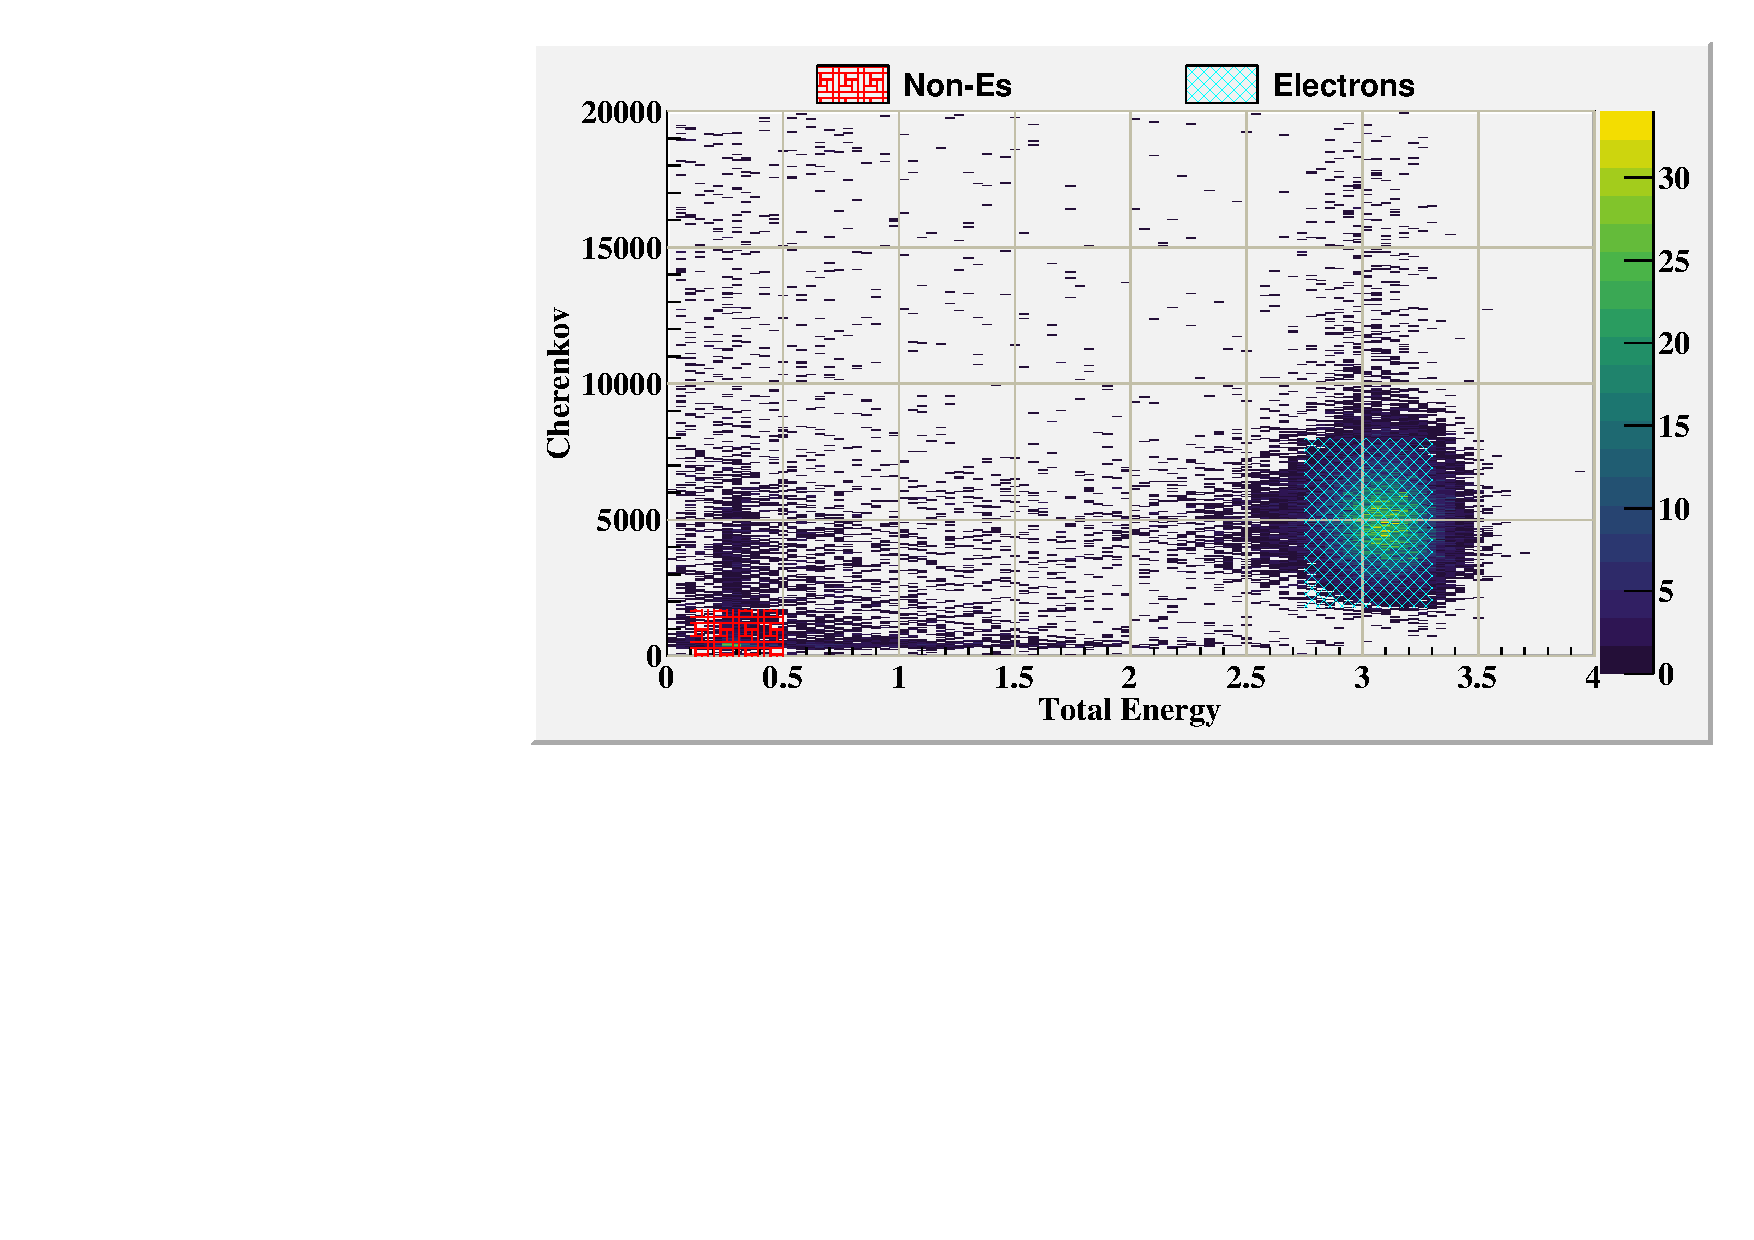
\includegraphics[width=13cm]{PID_2d}
	\caption{Two dimensional plot of the cherenkov sum versus Total Energy deposited, including electron sampling in teal and non-electron sampling in red. }
	\label{elesample}
\end{figure}

\begin{figure}[t]%
	{\centering
		\textbf{Particle ID and efficiency sampling for PID detectors }\par\medskip}
	\centering
	\subfloat[]{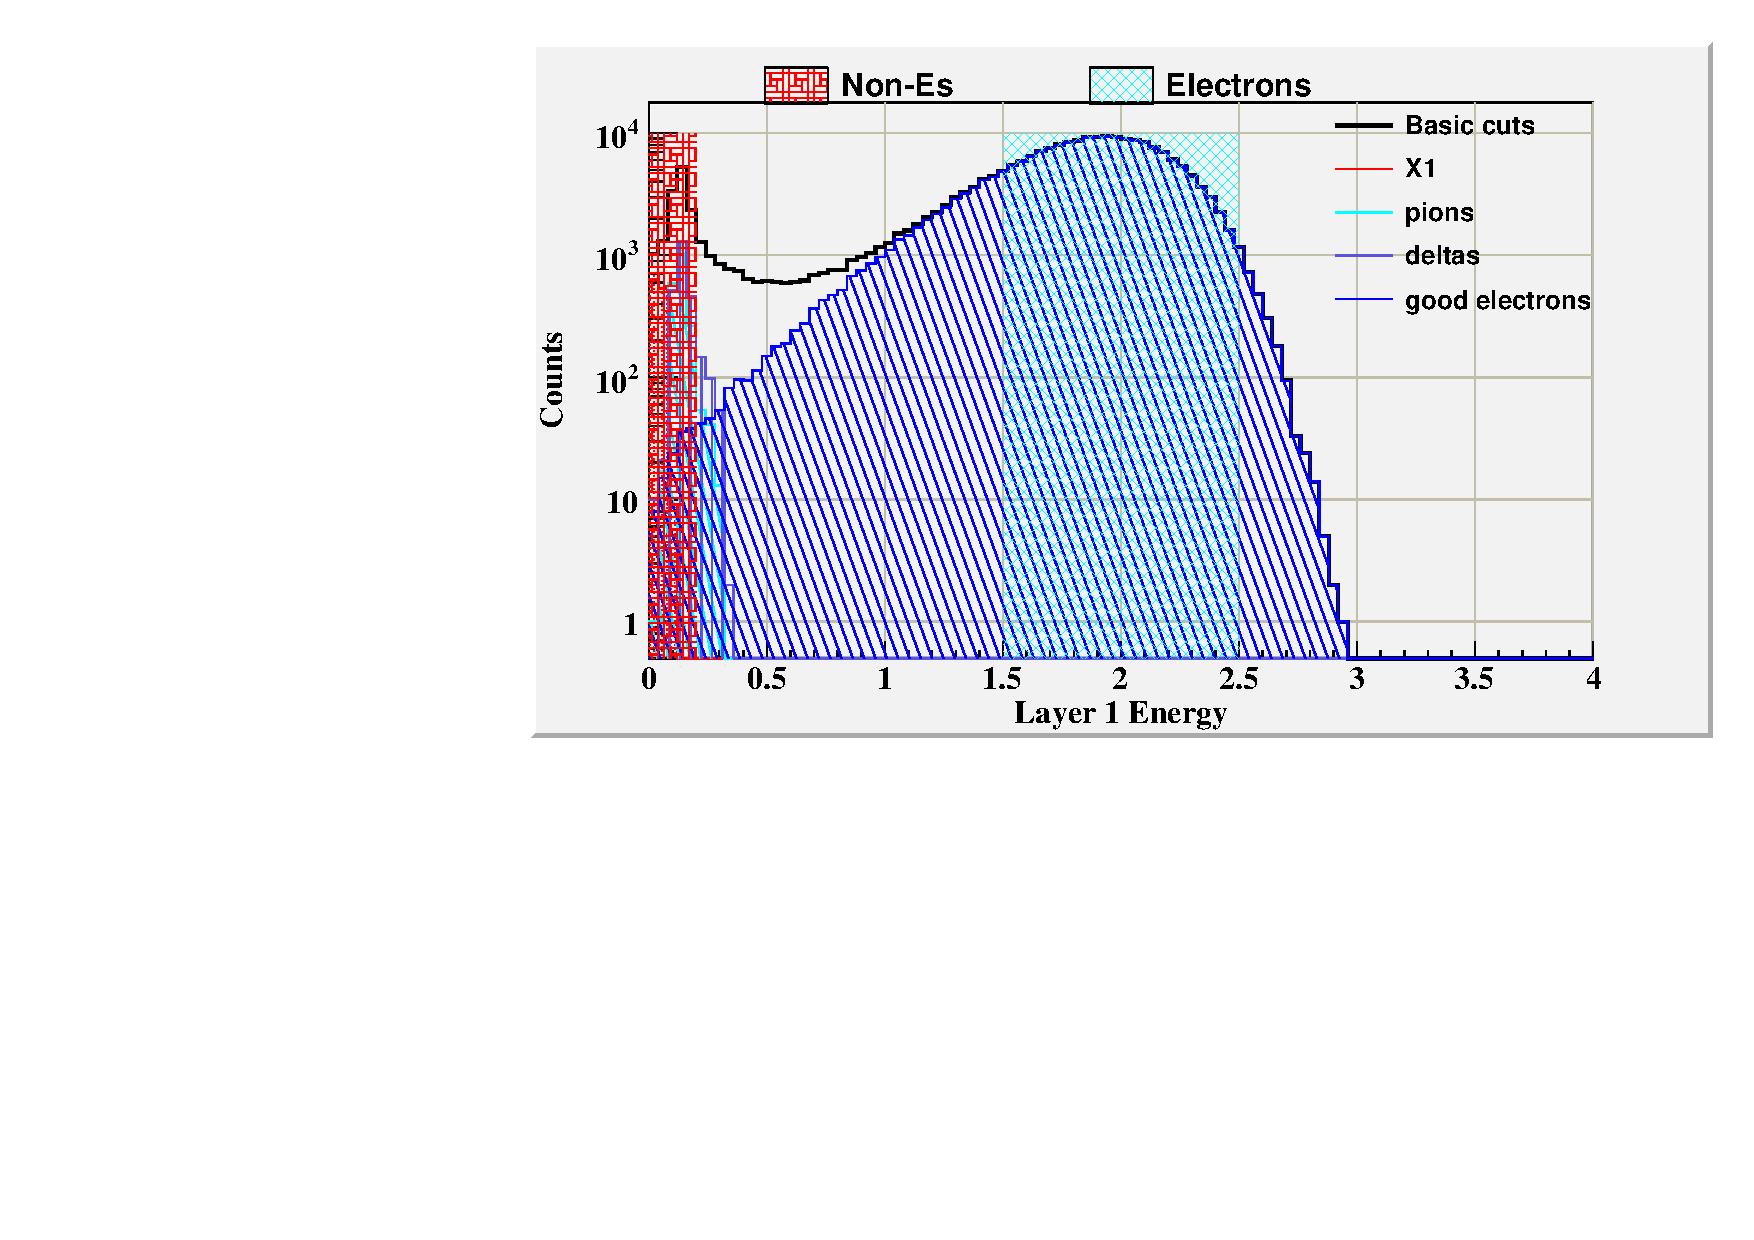
\includegraphics[width=0.5\textwidth,height=4.5cm]{Lprl1}\label{samA}}%
	\subfloat[]{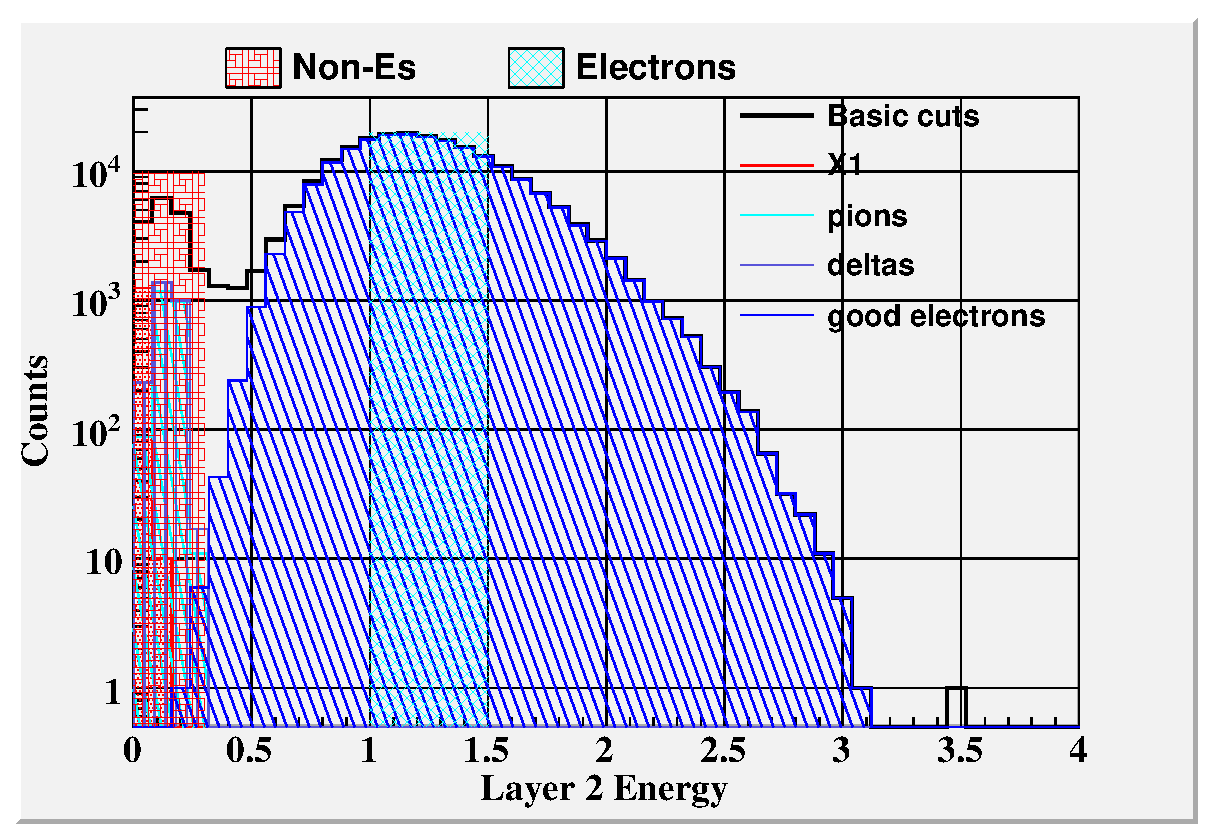
\includegraphics[width=0.5\textwidth,height=4.5cm]{Lprl2}\label{samB}}\\
	\subfloat[]{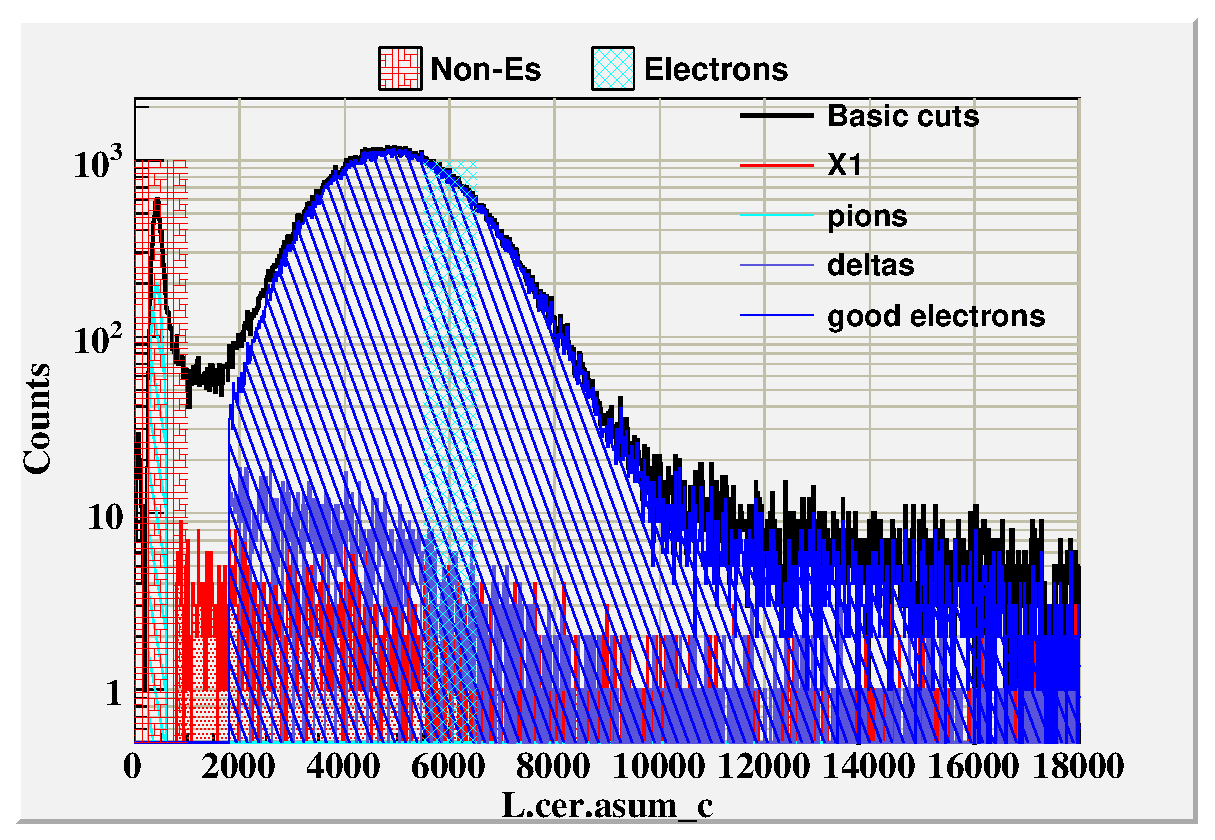
\includegraphics[width=0.95\textwidth,height=3.85cm]{Lcerasum}\label{samC}}%
	\caption{Electrons and other back ground particles identified via cuts in the total calorimeter and the gas cherenkov shown in the individual layers of the calorimeters and the cherenkov. Sampling cuts for Electrons in teal and Non-Electrons in red.}%
	\label{sampling}%
\end{figure}


\paragraph{}The efficiencies of the spectrometer's particle identification(PID) detectors were determined by using the first calorimeter layer, the second calorimeter layer, and the cherenkov to provide samples of good electrons and other particles. The PID efficiency of the individual detectors was determined using equation \ref{effequ}. The good electron sample for calculating the efficiency of the single detector was defined by sampling through the other two detectors. Sampling through the two layers of the calorimeter is shown in figure \ref{samA} for the first layer of the calorimeter and \ref{samB} for the second layer. The cherenkov good electron sample is shown in figure \ref{samC}. The electron sample from the cherenkov is contaminated by delta particles and a combination of unknown particles. These unidentified background particles are known to be relativistic due to the amount of light seen in the cherenkov. However, the events do not deposit enough energy into the calorimeter system to be considered as a good electron that scatter from our target through the detector. Using sampling in one layer of the calorimeter and the cherenkov, these unwanted low energy particles are rejected from sampling for efficiency calculations. The electron selection PID efficiency for the three PID detectors was determine at each kinematic setting to be approximately 98$\%$ . The efficiency was determined to be independent of the kinematic setting. Only small fluctuations were seen during the study, these small changes are due to decrease in statics, and all of the results fall within statical uncertainty of being independent of kinematic setting. The non-electron suppression efficiency was determine as part of this PID efficiency study to ascertain how many back ground particles leak into our sample of good electrons after cuts our made. The suppression efficiency of the cherenkov suffered due to the contamination of the relativistic low energy particles. Combining the two calorimeter detectors with the cherenkov increased the overall suppression efficiency for the spectrometer to 99.9$\%$ over the entire kinematic range of the MARATHON experiment. 

\begin{figure}[t]
	{\centering
		\textbf{PID efficency for each detector for all kinematics. }\par\medskip}
	\centering
	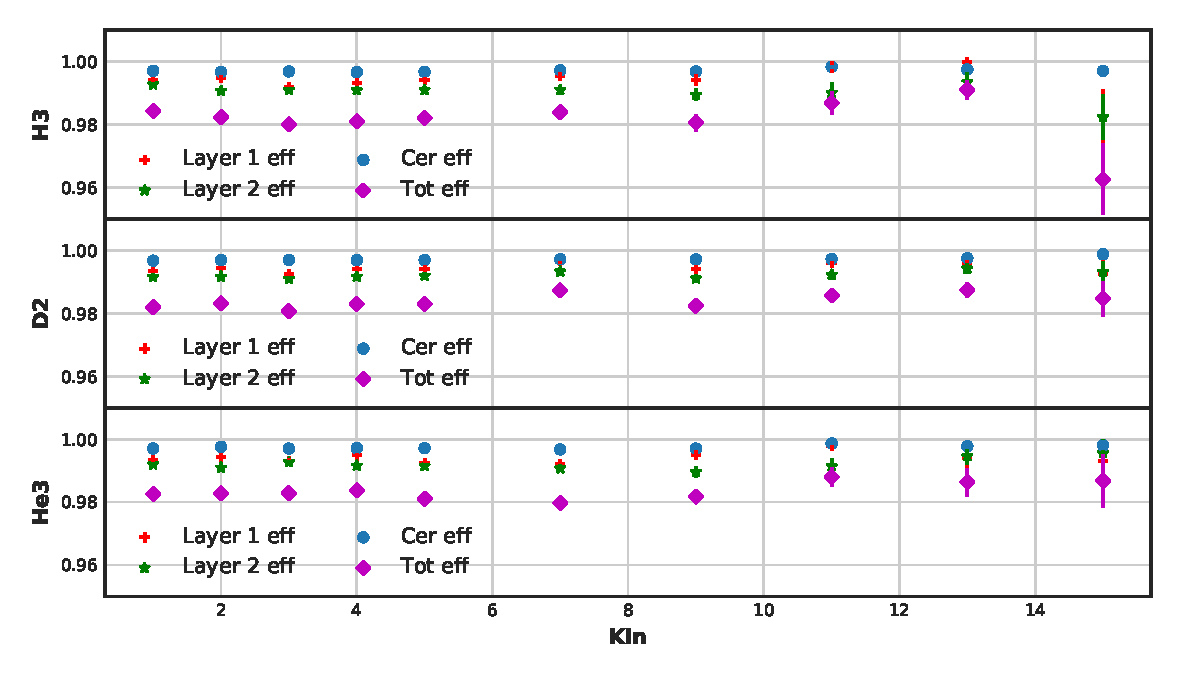
\includegraphics[width=15cm]{PID_allkin_alltgt}
	\caption{The PID efficiency for the cherenkov and both layers of the calorimeter,including the overall total PID efficiency for each of the gas targets at all of the kinematics.}
\end{figure}

\subsection{Trigger Efficiency}
\paragraph{} The process of capturing data from the two HRSs begins with the firing of a trigger. The trigger design for MARATHON focused on triggering for electrons and reducing the amount of other particles. Figure \ref{fig:trig_layout} describes the design of MARATHON's main trigger and efficiency triggers. MARATHON's main trigger, trigger 2, consist of a $(So \& S2) \& Cer$. Due to inefficiencies of the electronics, logic, and detectors an event can produce a false trigger or a high quality electron may not fire 
the main trigger.

\begin{figure}[]
	\centering
	\textbf{Trigger efficiency for the MARATHON experiment }\par\medskip
	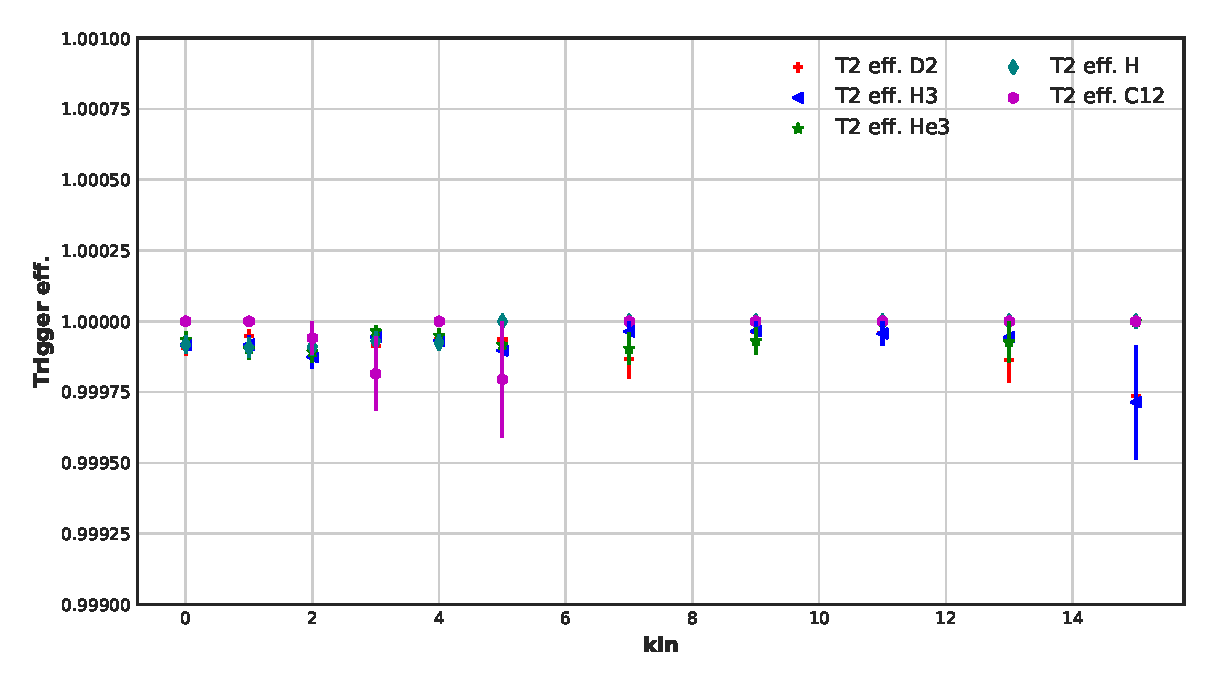
\includegraphics[width=14cm]{Trigger_Eff.eps}
	\caption{Trigger efficiency of trigger 2 for different targets at all kinematics calculated via sampling from trigger 1. }
	\label{trigeff}
\end{figure}

\paragraph{} A low threshold in the cherenkov allows for an inclusive trigger limiting the overall number of quality electrons missed, but allows for a large quantity of false triggers. Software PID cuts prevent the contamination of false positives from trigger inefficiencies. The tight PID software cuts removes the false positive inefficiency from the trigger design and is then considered in the PID efficiencies. The trigger inefficiency caused by missed high quality electrons was then calculated by sampling the high quality electrons in trigger 1, $(S_o \& S_2)$. This ties the efficiency of trigger 2 with the performance of the scintillators. The efficiency of the two scintillating planes in conjunction is calculated by using sampling in trigger 3, $(S_o | S_2) \& Cer$ with strict PID cuts in both layers of the calorimeters and requiring a hit in the cherenkov. The two scintillator planes in conjunction have an efficiency greater than $99.7 \% $ for all kinematics. Combining the trigger efficiency of the main trigger shown in figure \ref{trigeff} with the performance of the scintillators give an over all efficiency for the trigger of the MARATHON experiment of greater then $99.6\%$.

\subsection{Tracking Efficiency}
\begin{figure}[]
	\centering
	\textbf{Tracking efficiency for the MARATHON experiment }\par\medskip
	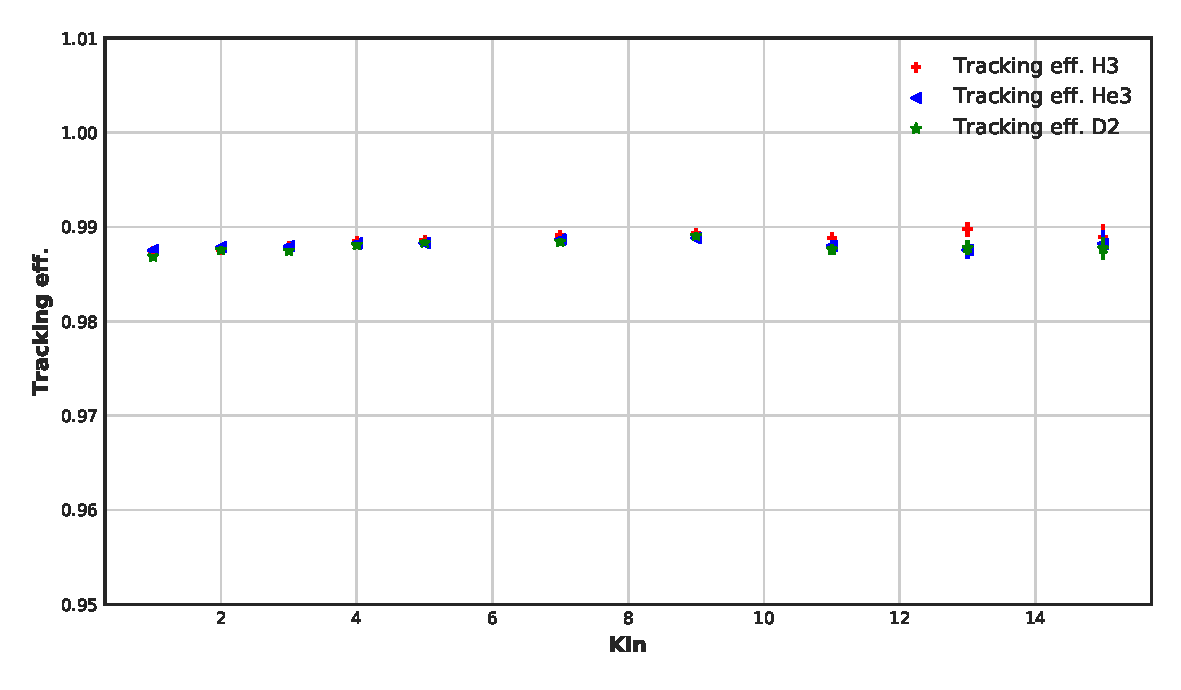
\includegraphics[width=15cm]{Tracking_Eff_allkin.eps}
	\caption{Tracking efficiency of the VDCs for different targets at all kinematics. }
	\label{trackeff}
\end{figure}
\paragraph{}Particles that travel through our detector could originated from sources wanted or unwanted. In order to control the source of the scatter electrons, we use a particle's track to identify its source. The signals received via the VDC is used to produce a particles track from the target to end of the spectrometer. The largest source of inefficiency for the VDCs are incorrectly identified tracks. High quality electrons that transverse the spectrometer should only have one good track, calculated via the tracking package in the analysis software. The capability of the VDCs to determine a good electron event's one good track is know as the one track efficiency for the VDCs. Quantitatively the one track efficiency ($\epsilon_{VDC}$) can be obtained via:
\begin{equation}
\epsilon_{VDC} \equiv \frac{N_{1 track} }{N_{all}}
\end{equation}
Where the number of good electron events that have one good track is defined as $N_{1 track}$, and $N_{all}$ are all of the electrons rather they have a good track or not. The good electron selection is made via PID cuts in the calorimeter and cherenkov, and cuts in the ADC and TDC of the scintillators. Direct cuts in the signal of the scintillators where made to include the nominal acceptance cuts, which our produced through tracking software. The tracking efficiency of HRSs during the MARATHON experiment is shown in figure \ref{trackeff} for the three gas targets during all kinematic ranges. The efficiency of the VDCs is not relative to the angle of the spectrometer. So the uniform tracking efficiency across all kinematics is expected and helps eliminate any concerns of the performance of the VDCs during the experiment. 

\section{Background Subtraction}
\paragraph{} The purpose of this analysis is to study the DIS cross sections of deuterium, helium-3, and tritium. The sample of scattered events used to determine the cross section of a given nuclear target then needs to be cleaned of any contamination produced from other targets and processes. The electrons detected by the spectrometers can be electrons that scatted from our chosen target, scattered from a source other then our target, or produced through process other than DIS scattering. The two sources of contamination for the MARATHON experiment are events scattered from the aluminum end caps of the target cell and pair produced electrons via photon interaction. 
\subsection{End Caps}
\paragraph{} The target cells used during the MARATHON experiment are shown in figure \ref{HATT}. The majority of the events from the end caps can be removed easily via a cut in the reconstructed quantity of reaction vertex along the beam axis. The relatively large density thickness of the aluminum end caps cause a large amount of end cap contamination. The majority of the electrons that scatter from the end caps can be removed through software cuts in the reaction vertex along the beam axis(z). Show in figure \ref{EC5} is a comparison of the reaction vertex of the electron events between the gaseous targets and the empty cell target at kinematic 4. The yield is normalized by the number of event in the histogram to remove any bias from the amount of time of beam on target. The empty target  results in figure \ref{EC5}, demonstrate the form of scattering off of the aluminum windows of our target cell. Using the reconstructed vertex location of the scattering origin, the vast majority of the events from the windows can be removed. This vertex cut is shown by the two vertical blue lines. Only events that lie within these two line are considered good electrons from our chosen target. 


\begin{figure}[]
	\centering
	\textbf{Scattering vertex along the beam axis. }\par\medskip
	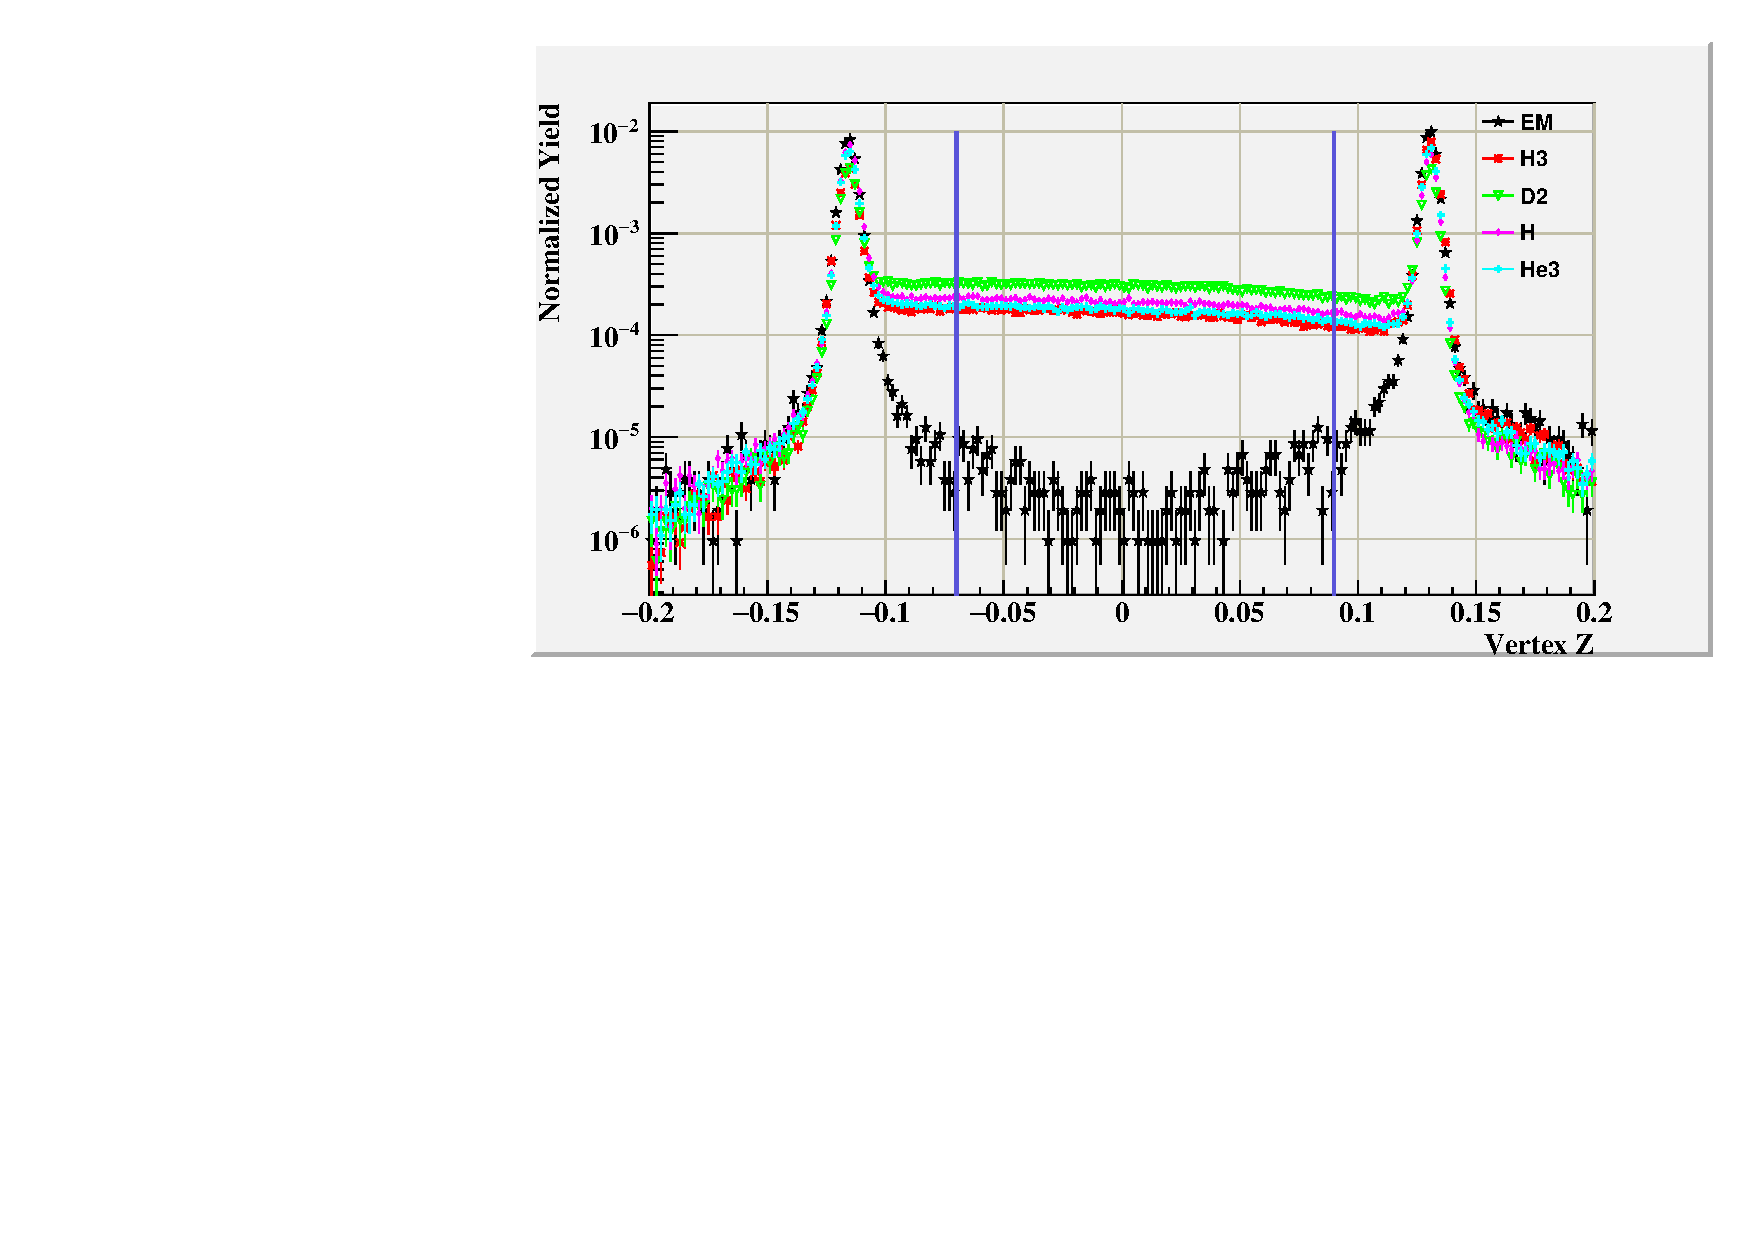
\includegraphics[width=15cm]{endcap_kin4.pdf}
	\caption{Comparison of the scattering vertex along the z axis for the empty target(EM) and the gas targets at kin. 4. }
	\label{EC5}
\end{figure}

\paragraph{}The empty cell vertex z disruption does have content within the vertex cut. These events that remain after the cut are corrected for via an end cap contamination factor. This  factor is calculated by determining the ratio of the number of good electrons that scatter from the empty cell and from each gas cells, resulting in ratio of $\big(\frac{Yield_{EC}}{(Yield_{Gas} + Yield_{EC})}\big)$. Where the subscript EC denotes events from the end caps. The correction factor applied to the yield calculation is defined as:
\begin{equation*}
ECC = 1- \big(\frac{Yield_{EC}}{(Yield_{Gas} + Yield_{EC})}\big) \equiv \frac{Yield_{gas}}{(Yield_{Gas} + Yield_{EC})}
\end{equation*}

%\begin{table}[]
%	\textbf{End cap contamination for each target at all kinematics. }\par\medskip
%	\hspace{-70pt}
%	\begin{tabular}{|l|l|l|l|l|l|l|l|l|l|l|}
%		\hline
%		Kinematic  & 1       & 2       & 3        & 4        & 5        & 7       & 9       & 11       & 13       & 15   \\ \hline
%		H3   & 0.0218 & 0.0202 & 0.0163   & 0.0154   & 0.01445  & 0.01177 & 0.009   & 0.0069   & 0.0055   & 0.0043     \\ \hline
%		He3  & 0.0251 & 0.0229 & 0.01839  & 0.01727  & 0.01573 & 0.0125  & 0.00974 & 0.00715  & 0.00572 & 0.00449  \\ \hline
%		D2   & 0.0113 & 0.010  & 0.008206 & 0.00934 & 0.00864  & 0.00831 & 0.0057  & 0.00512 & 0.00379  & 0.00276   \\ \hline
%		H    & 0.0238  & 0.020 & 0.0178   & 0.0176   &          &         &         &          &          &            \\ \hline
%	\end{tabular}
%	\caption{The amount of electrons that scatter from the empty cell compared with the amount electrons that scatter off a gas filled cell. }
%	\label{ECCtable}
%\end{table}



\subsection{Pair Produced Electrons}
\paragraph{} The high energy scattering interaction used to create deep inelastic scattering events can produce high energy photons and pions. The high energy photons that have energy greater than 1.022 MeV can convert into e$^+$e$^-$ pairs when the photons interact with a medium. A correction for the number of back ground electrons produced via a pair production process was calculated by determining the amount of positrons produced from equal targets and kinematics. The yield of positrons were measured for kinematics one through five. The results were used to construct a function to determine the amount of contamination at high $x_{Bj}$ kinematics. Figure \ref{PC} shows the amount of positron contamination for tritium and an exponential fit to extrapolate over the entire ranged in $x_{Bj}$ for the MARATHON experiment. 

\begin{figure}[h]
	\centering
	\textbf{Tritium positron contamination. }\par\medskip
	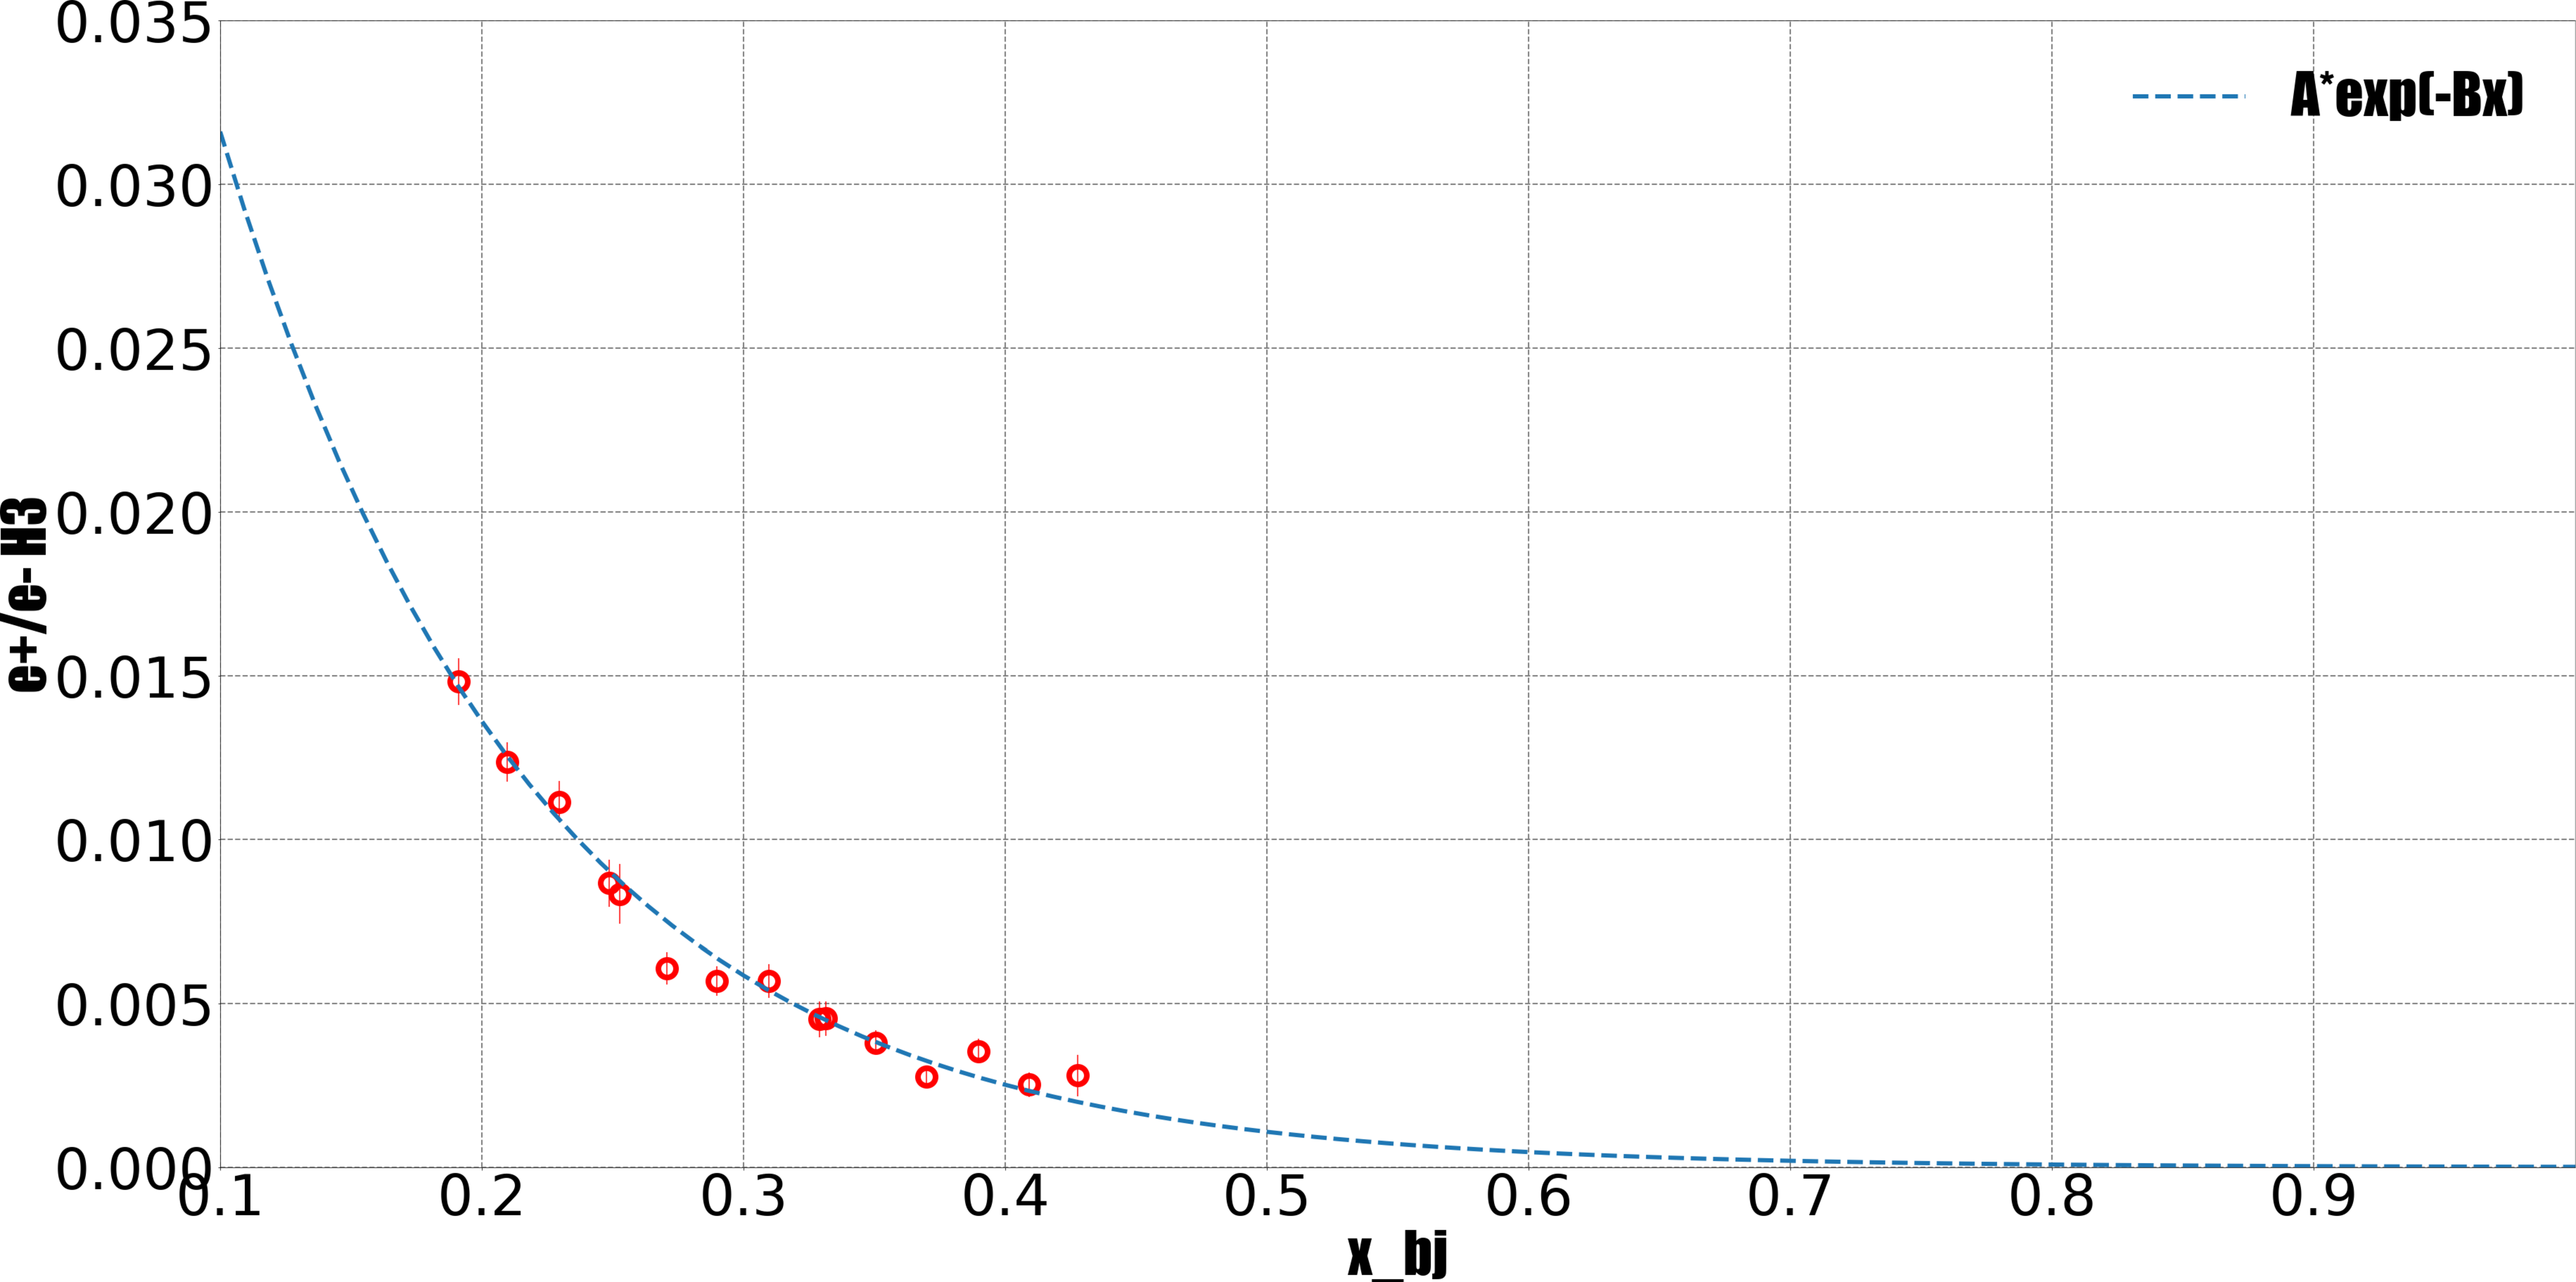
\includegraphics[width=15.0cm]{../images/positron_H3_bane.pdf}
	\caption{The ratio of positron events to electrons for tritium \cite{tongsu}. }
	\label{PC}
\end{figure}

\subsection{Beta Decay of Tritium}
\paragraph{} Tritium a radioactive isotope of hydrogen will beta decay to $^3$He. Tritium has a half-life of 4500 $\pm$ 8 days \cite{T2HL}. The gas cell used to contain Tritium for the experiment was filled on October 23, 2017. The initial tritium thickness density of our tritium cell was $0.077 \pm 0.001 $ grams per cm$^2$. Tritium will decay to $^3$He via a beta interaction. The tritium in our cell is diatomic and decays via two channels\cite{diaT}. The possible decay channels and their branching probabilities are shown in equation \ref{branching}. In DIS interactions, the molecular effects are ignored due to the size of the probe in a DIS scattering event which allows for the different channels to be treated as one. 
\begin{align}
			^3H_2 &\rightarrow(^3H ^3He)^+  &(94.5 \pm 0.6\%) \nonumber \\ 
			^3H_2 &\rightarrow(^3H)^+ + (^3He)^+  & (5.5 \pm 0.6\%) 
			\label{branching}
\end{align}
\paragraph{}The amount of $^3$H and $^3$He in our tritium cell will change in respect to the time since the feeling of the cell. Equations \ref{nT} and \ref{nH} describe the amount of $^3$H and $^3$He in the tritium cell has a function of the time since fill date and the original amount of $^3$H and $^3$He in cell at filling. In equations \ref{nT} and \ref{nH}, $n_T(n_H)$ is the time dependent amount of tritium(helium), and  $n_T^0(n_H^0)$ is the amount of tritium(helium) in the cell at time of filling. t is the time since the cell was filled and $\tau$ is the mean lifetime of tritium.
\begin{align}
	n_T &= n_T^0 \: e^{-t/\tau} \label{nT}\\
	n_H &= n_H^0(1 - e^{-t/\tau}) \label{nH},
\end{align}
As time passes the amount of $^3He$ increases, the contamination becomes a non-negligible effect on the yield of scattered electrons. The fraction of $^3He$ in the tritium can reach up to 3$\%$ for the data from the end of the MARATHON experiment. This $^3He$ fraction as a function of time is shown in figure \ref{Hfract}, with the period for running the MARATHON experiment labeled as a color band. 

\begin{figure}[t]
	\centering
	\textbf{Helium Fraction from Tritium Cell. }\par\medskip
	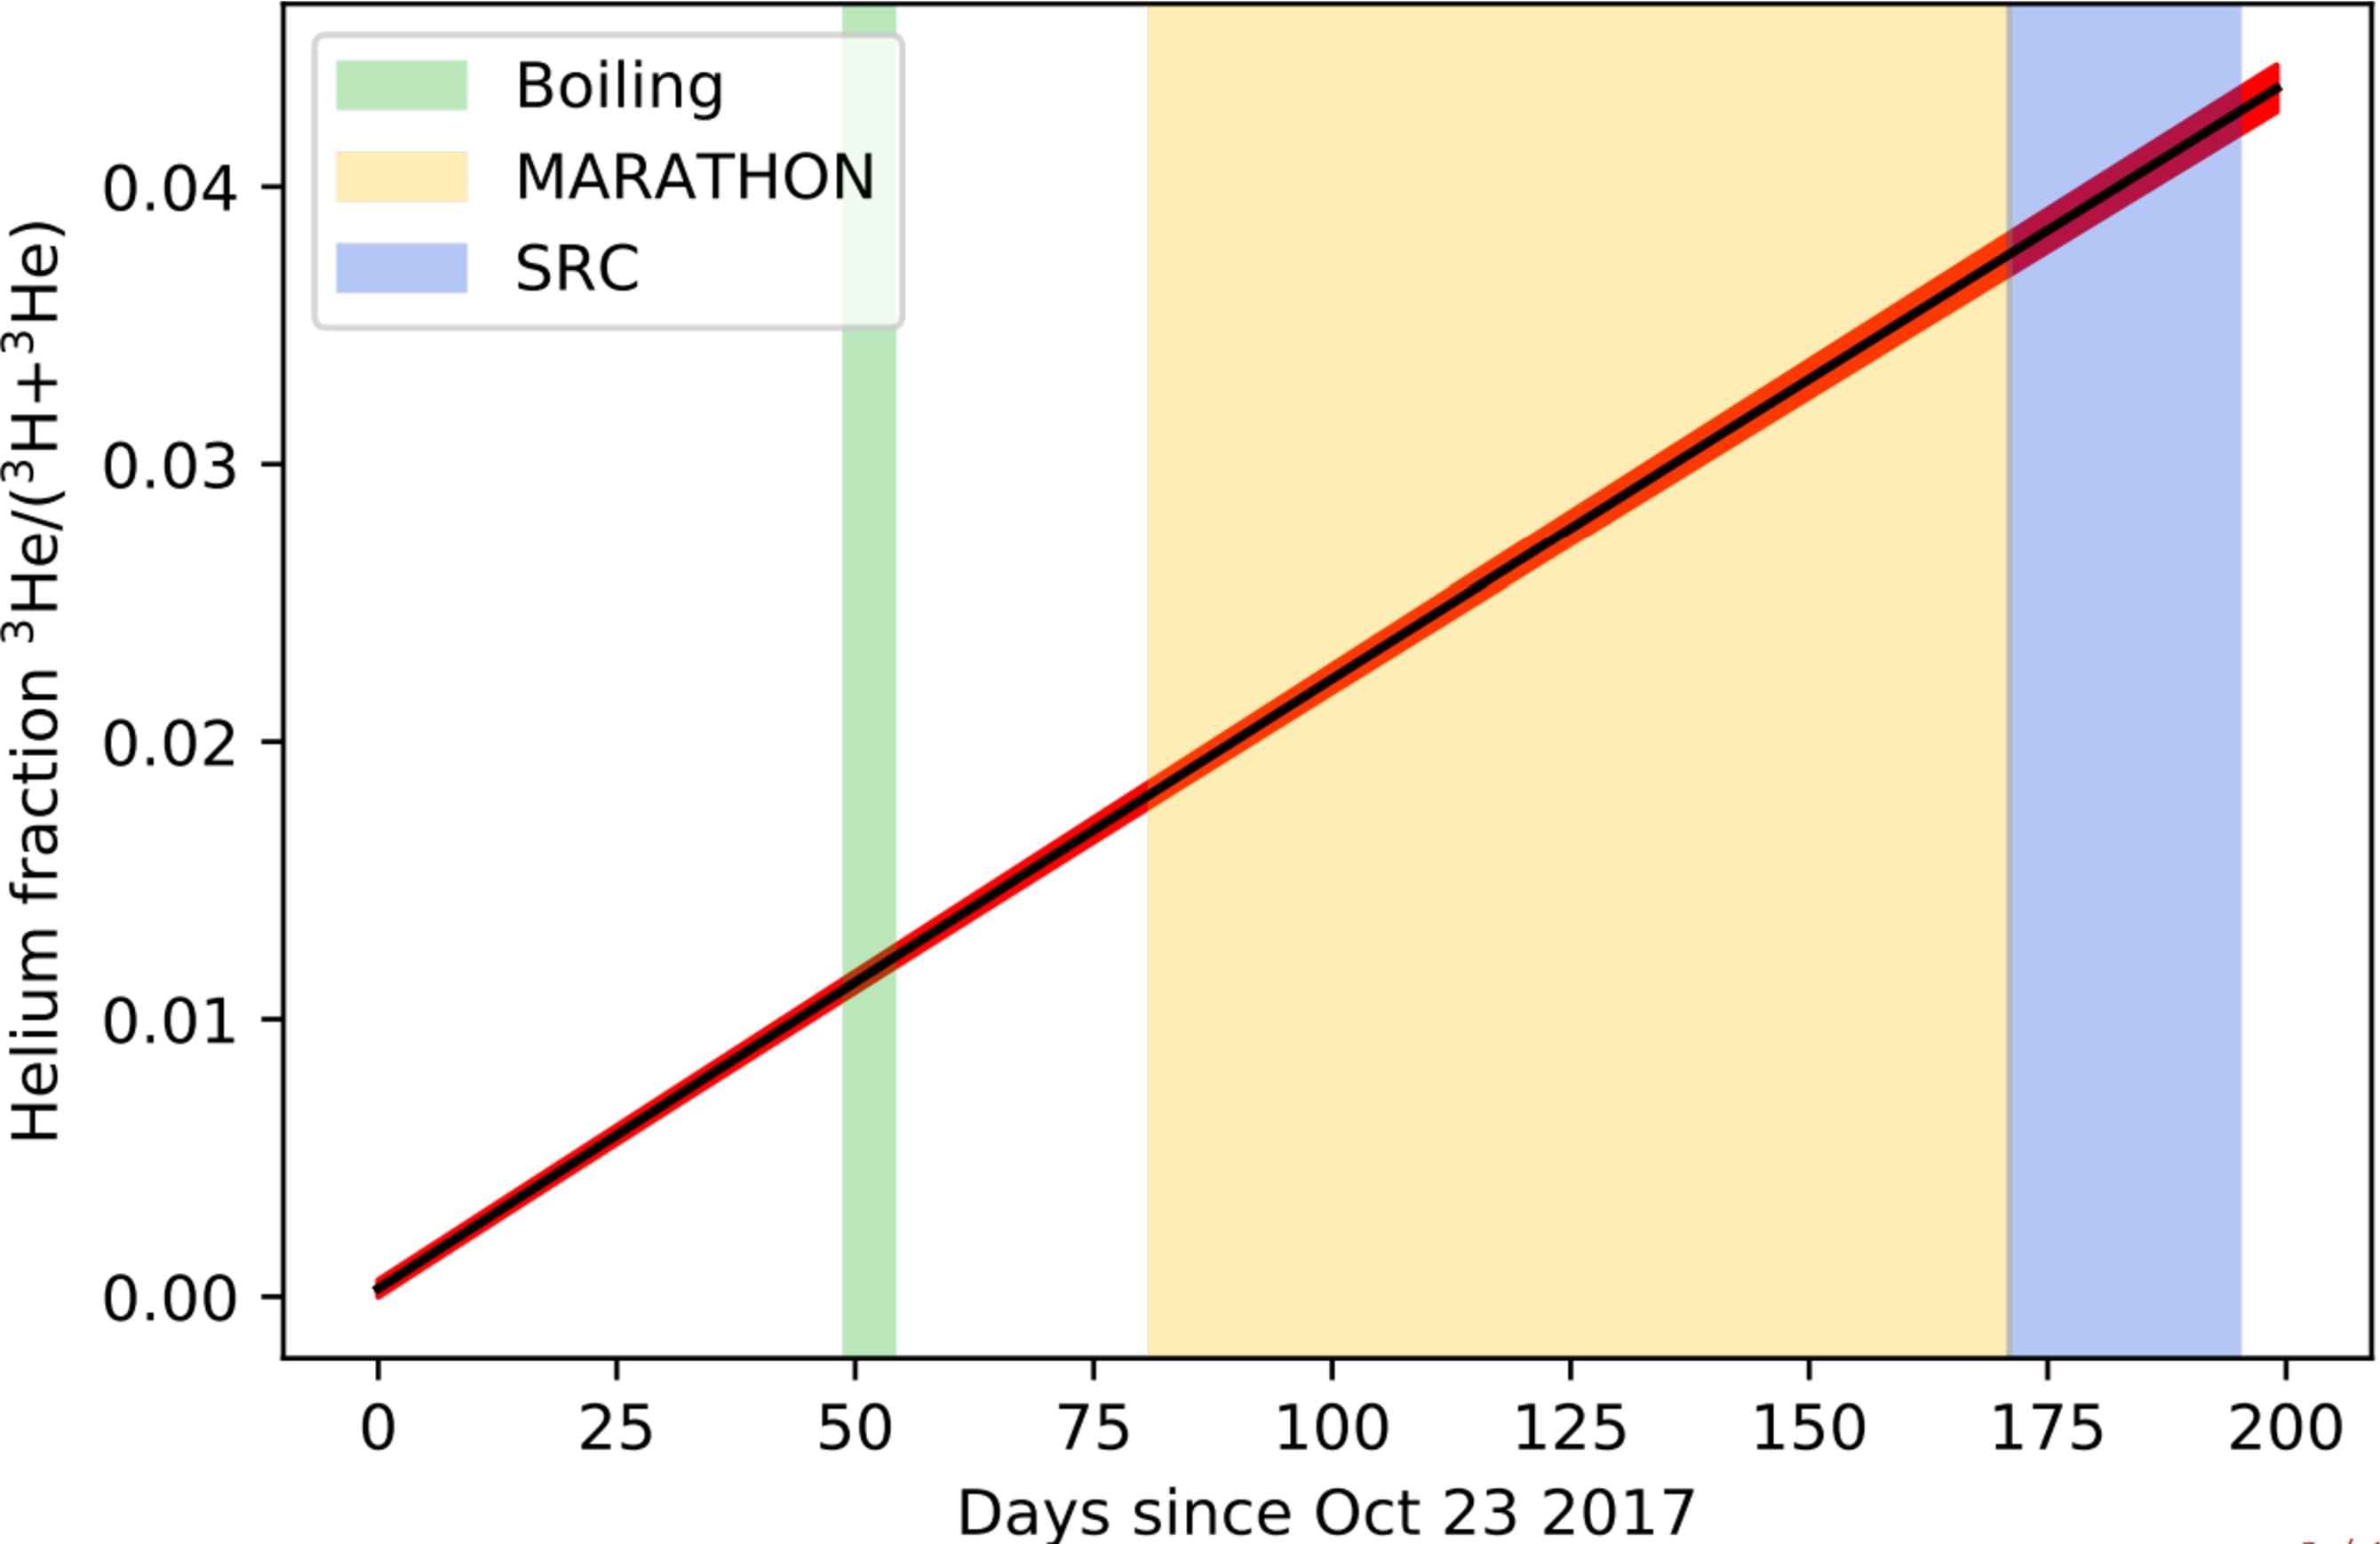
\includegraphics[width=13cm]{cont_Hfrac.pdf}
	\caption{The amount of Helium in the Tritium cell in reference to the total amount of material in the cell as a function of time. Included are bands of time for different sections of the Tritium run group's plan \cite{Beta}.}
	\label{Hfract}
\end{figure}
\begin{equation}
Y = \frac{\sum N_i}{\sum Q_i n_i}, \label{yield} 
\end{equation}
\begin{equation}
Y_{raw} = \frac{\sum (T_i + H_i)}{\sum Q_i (n_{T,i} + n_{H,i})} \label{Yraw}
\end{equation}
\begin{equation}
\langle f_H \rangle \equiv \frac{\sum Q_i f_{H,i}}{\sum Q_i} \label{QwHf}
\end{equation}


The events that scatted from Helium in our tritium cell need to be subtracted from the measured yield to supply an accurate count. The yield from any target is defined as the number of electrons per charge weighted scattering centers. The yield is shown in equation \ref{yield} and defined as the number of counted events($N_i$) per possible scattering changes, or charge($Q_i$) times number of scattering centers ($n_i$). Data is recorded in many runs, so a sum over runs($i$) is required to get the total yield. The subtraction factor is calculated by breaking down the yield from the tritium cell as the addition of the yield from tritium ($Y_T$)= $\Sigma(T_i/Q_in_{i})$ and helium ($Y_H$)= $\Sigma(H_i/Q_in_{i})$ in the tritium cell as shown in equation \ref{Yraw}. The correction for the beta decay is defined in equation \ref{YieldT}. It can be determined by expanding equation \ref{Yraw} out and solving for the tritium yield from the tritium cell. Where $\langle f_H \rangle$ is the charge weighted helium fraction defined in equation \ref{QwHf} \cite{primer}. The helium fraction $f_{H,i}$ is the ratio of helium scattering centers in the tritium cell to total number of scattering centers. 

\begin{equation}
Y_T = Y_{raw}\left(\frac{1}{1-\langle f_H \rangle}\right) - Y_H \left(\frac{\langle f_H \rangle}{1-\langle f_H \rangle}\right) \label{YieldT}
\end{equation}

\section{Luminosity}

\section{Monte Carlo Ratio Method}
Use ECs slides need cite ,explain how to get CS from data/MC

\subsection{Monte Carlo Simulation}
gen - table -weight
\subsection{Monte Carlo Comparison}
acc - comp
\section{DIS Cross Section}

\section{Systematic Error}
\cite{Ar_Ti}





    	
\chapter{Results}
The culminating part of this nuclear physics analysis begins with the extraction of the experimentally measured DIS cross sections for three targets. Then using those cross sections to study the per nucleon scaled A/D ratio. I will also use these A/D ratios to study the EMC effect for both helium-3 and tritium. In this chapter, I will present my results for the DIS cross sections and EMC effect. I will also discuss an error analysis for both the cross section measurements and the EMC effect results. 
\section{DIS Cross Section}
\paragraph{}Using the Monte Carlo ratio method, I extracted the experimental measured cross section for helium-3, tritium, and deuterium. These DIS cross section extraction ranges from 0.18 to 0.82 in $x$, from 2.2 to 11.8 GeV$^2$ in $Q^2$, and has W$^2$ $>3.5$ GeV$^2$. The central momentum setting of the spectrometer was 3.1 GeV/c and the spectrometer was moved from 17.5 to 33.5 degrees.

\begin{equation}
\sigma_{Data} = \sigma_{model} \cdot \frac{Y_{Data}}{Y_{MC}}. \nonumber
\end{equation}
%\begin{landscape}
%\begin{sidewaysfigure}
\begin{figure}
%	\hspace{-80pt}
	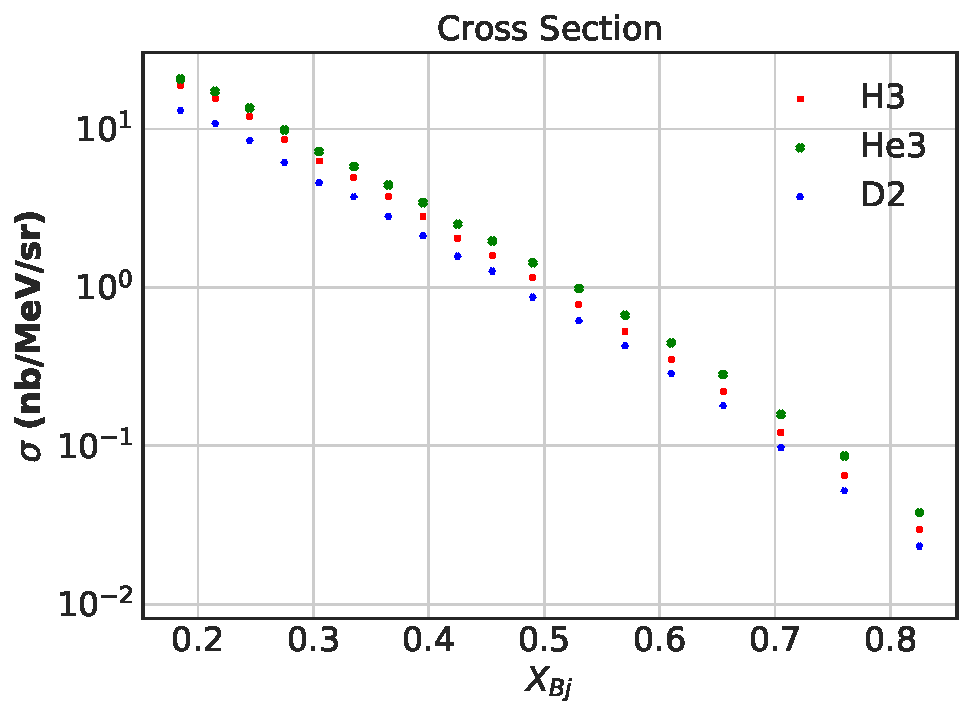
\includegraphics[width=15.5cm]{../images/total_xs.pdf}
	\caption{Experimentally measured cross section using the Monte Carlo ratio method for tritium, helium-3, and deuterium. Normalization uncertainty due to target thickness uncertainty for tritium= 0.97\%, helium-3 = 1.12\%, and deuterium = 0.56\%.}
    \label{CCplot}
\end{figure}
%\end{sidewaysfigure}
%\end{landscape}
I compared the data yield to the Monte Carlo yield to produce a correcting factor for the model cross section. Figure \ref{D_MC_COMP} shows the ratio comparison between data and Monte Carlo in bins of $x$. Then apply the ratio factor for a bin in $x$ to the model cross section to extract out the experimentally measured cross section for that bin. Figure \ref{CCplot} shows a plot of the experientially measured cross section for tritium, helium-3, and deuterium. 


\section{Cross Section Error Analysis}
The measurement of the cross section requires finally tune detectors and analysis process. Uncertainties arise due to the nature and limitations of the spectrometers and the analysis of the data received. In this section, I will discuss the calculation and propagation of errors in the analysis of the DIS cross section. The error analysis will be broken into the calculation of normalized yield for data, yield for Monte Carlo, and the cross section extraction. 
\begin{table}[]
	\caption{Relative Error Contributions in $\%$ for Cross Section for a selection of bins. The efficiency error is a combination of the error from the livetime, PID, tracking, and trigger efficiency calculations.}
	\centering
	\begin{tabular}{|l|l|l|l|}
		\hline
		\textbf{\qquad \qquad\qquad x bin}   & \textbf{0.215} & \textbf{0.455} & \textbf{0.705} \\ \hline\hline
		Statistical             & 0.512 & 0.889 & 1.106 \\ \hline
		Efficiency Error*       & 0.665 & 1.477 & 2.951 \\ \hline
		Positron Correction     & 0.036 & 0.016 & 0.005 \\ \hline
		End cap Correction     & 1.0 & 1.0 & 1.0 \\ \hline
		Charge Calculation     & 0.2 & 0.2 & 0.2 \\ \hline
		Density Correction      & 0.2 & 0.2 & 0.2 \\ \hline
		Monte Carlo Statistical & 0.193 & 0.217 & 0.209 \\ \hline
		Optics Reconstruction	& ?0.665& ?1.477 &?2.951 \\ \hline
		??Cross Section Model 	& ?0.193 & ?0.217 & ?0.209 \\ \hline
		??Radiative Corrections\cite{primer} 	& 0.5  & 0.5 & 0.5 \\ \hline
		Total Error		 	 	& 0.95  & 1.931 & 3.316 \\ \hline
	\end{tabular}
\end{table}

\begin{align}
\dfrac{d\sigma}{dE^{\prime}d\Omega} &= \frac{(N - BG)}{\mathscr{L} \cdot \epsilon \cdot \Delta E^{\prime} \Delta \Omega \cdot A(E^{\prime},\theta)}. \nonumber\\
\sigma &= \text{NormY}/\left(\Delta E^{\prime} \Delta \Omega \cdot A(E^{\prime},\theta)\right)\nonumber\\
\text{NormY} &= \left(N_e \cdot BG/\epsilon \right) / \mathscr{L}
\end{align}
\subsection{Normalized Yield Error}
\subsubsection{Corrected Electron Count Error}
\paragraph{}
The contributions for error on the measurement of the normalized yield(normY) can be simplified into the contributions for the corrected number of electrons and the luminosity. The error for the corrected number of counted electrons includes the random statistical error for the count of electrons detected, the error associated with the calculated efficiencies, and the error from the background correction. The electron statics range from 4875 to more then 42000 in a bin and therefor I have treated the randomness of the counting in a standard error technique. The relative statistical error for a bin is $\frac{1}{\sqrt{Ne}}$ and ranges from .5\% to 1.4\%. Calculating the efficiencies deals with calculating a probability of a binomial choice. The errors associated with the efficiencies are calculated using the Wilson score interval described in equation \ref{WSI}, where $p$ is the efficiency or a probability of a success, $n$ is the number of samples, $z$ is 1.645 for a 95\% confidence level. 
\begin{equation}
p[_{UpperBound},_{LowerBound}] = \frac{ 2np +z^2 \pm \left[z\sqrt{z^2 - \frac{1}{n} + 4np(1-p) +(4p-2)} + 1 \right]}{2(n+z^2)} \label{WSI}
\end{equation}
The relative efficiency errors are added in quadrature to calculate an over all efficiency error to be propagated into the yield calculation.
\paragraph{}The correction for background events corrects for events from the end caps and pair produced electrons. The end cap correction factor is produced by a ratio of yields between the gas cells and the empty cell. This yield measurement allows for the cancellation of many of the systematic uncertainties. The largest contribution to the this error is the low statistics of the back ground events. The estimated error to the cross section analysis is about 1\%. Furtherer study of the end cap contamination and the error associated with the correct is part of the ongoing analysis. The error for the positron correction involves using the covariance matrix for the exponential fit and propagating the error for each parameter of each target using the $x_{Bj}$ dependent function. The error for the fit parameters are propagated to an error for the correction using equation \ref{cv_err}.
\begin{equation}
\frac{\Delta f(x)}{f(x)} =  \sqrt{ \sum_{i}^{} \left(\delta p_i\cdot x^i\right)^2 + \sum_{ij}^{}\left( 2\cdot \delta p_{ij}\cdot \dfrac{df(x)}{dp_i}\cdot \dfrac{df(x)}{dp_i}\right) } \label{cv_err}
\end{equation}
The error for the background corrections are added in quadrature to get an overall error for the total back ground correction.  
\subsubsection{Luminosity Error}
\paragraph{}The errors involved in the luminosity calculated is the target density thickness measurement, beam charge calculation, and density correction. The error in the target thickness measurement is considered a overall normalization uncertainty. The error for the three gas targets' thickness measurements are: tritium= 0.97\%, helium-3 = 1.12\%, and deuterium = 0.56\% \cite{HATT_eng}. The measurement uncertainties for each gas target are displayed in table \ref{tgt_table}. The amount of beam charge deposited on the target is calculated via the BCM(beam charge monitors) and their calibrations. The BCM calibrations were determined a few times through the run period with no change to the calibration constants. Due to the consistency of the BCMs and the high quality calibration the  error estimation for charge calculation is approximately 0.2\%. The error for the density correction is based in the error from the 2nd order polynomial fit. The error is calculated using the same method as the positron background correct, combining the errors for the fit parameters and the covariance terms through the propagation formula \ref{cv_err} using the current dependent correction function, \ref{eq:dc}. The relative error in charge on target and density correction have been added in quadrature to calculate a systematic error for the luminosity calculation. The systematic error for the luminosity and the systematic error for the correct count of electrons are then added in quadrature to calculate and overall normalized yield error.  
\subsection{Monte Carlo Yield Error}
\paragraph{}The responsibility of the Monte Carlo is to accurately account for the acceptance of the spectrometers. The uncertainty for thee Monte Carlo yield combines the statical uncertainty of the number of events generated and the reconstruction of the momentum and angle.  The statistical uncertainty is reduced due to the generation of a few million events. The uncertainty in the reconstruction of an event is a mixture of the uncertainties in the beam x and y position, spectrometer offsets, beam energy, optics, and acceptance cuts. The uncertainties for the beam x and y position was controlled by the BPMs and the calibration I completed. The uncertainty for the BPM measurements is 140 $\mu$m. The beam energy measurement is quoted to have an absolute accuracy of 5 x 10$^{-4}$.  The optics are capable of determining the relative in-plane angle with an accuracy of $\pm$ 0.2 mrad, out-of-plane angle with $\pm$ 0.6 mrad in the target coordinates, and momentum reconstruction 2.5x10$^{-4}$\cite{HallA}.  Using equation \ref{scatangle}, I propagated the resolution of target reconstruction variables to determine the relative uncertainty of the scattered angle to be $\approx$ 0.15\%. I have calculated the effect of the accuracy of the optics by comparing the cross section for the nominal values of , beam energy, scattered angle, and momentum, to the cross section of these values shifted by their uncertainties. A summary of the uncertainties used in the uncertainty of optics reconstruction.
\begin{itemize}
\item$\delta \theta$ = 0.15\%
\item$\delta E^{\prime}$ = $\pm$0.00025
\item$\delta E_{beam}$ = $\pm$0.0005
\end{itemize}


\cite{Ar_Ti}
\subsection{Cross Section Model Error}
\paragraph{}
The model dependence of the DIS cross section and the radiative corrections are the two factors of the systematic error that accompanies the Monte Carlo ratio method. My analysis of the model depended errors used different DIS cross section models to supply an error for the model cross section and the radiative corrections.

\section{EMC Ratios}
\paragraph{}In this section, I will present the A/D cross section ratios for helium-3 and tritium. The ratios are normalized by the number of nucleons in each target. Included in figure \ref{ADplot} are results from E03103. These results have different invariant mass but are considered DIS until 0.65 in $x$. Above this threshold, the invariant mass begins to drop lower then the DIS criteria used for my analysis. 
%\begin{landscape}
%\begin{sidewaysfigure}
%\thispagestyle{empty}
%\raisebox{-14.5cm}{\makebox[\linewidth]{\thepage}}
\begin{figure}
	\centering
	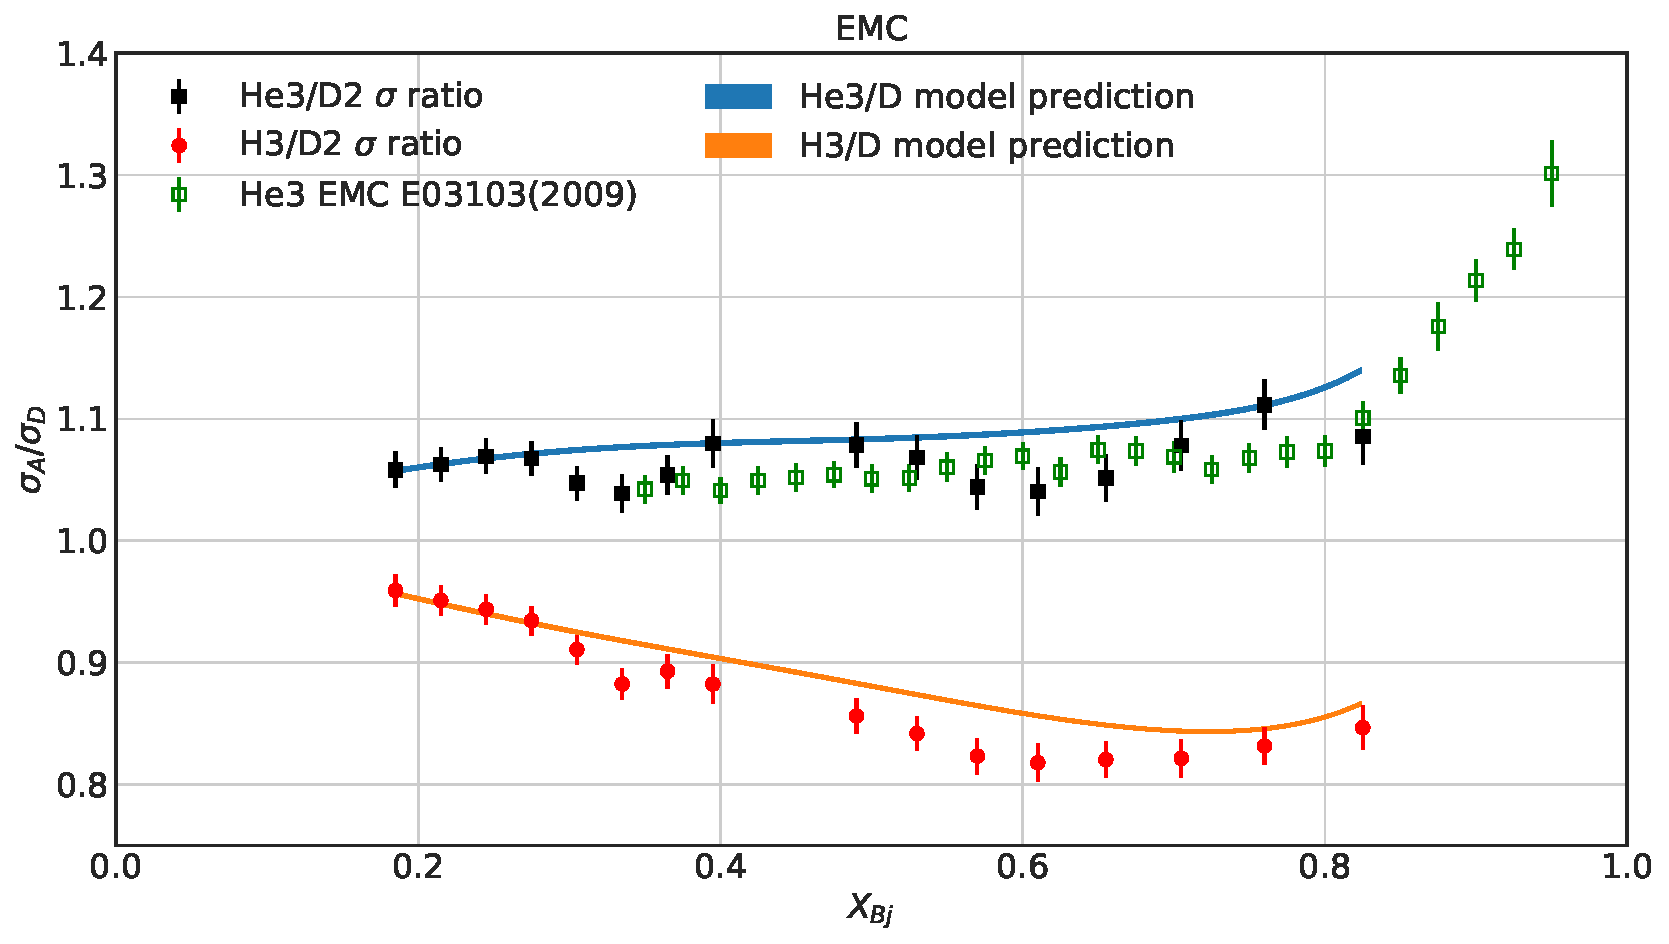
\includegraphics[width=15.5cm]{../images/A_D_ratios.pdf}
	\caption{The A/D ratio for helium-3 and tritium from my analysis. Also included, EMC analysis from E03103\cite{seeley} and the EMC ratios from a DIS scattering model from Arie Bodek model \cite{DISmodel}.}
	\label{ADplot}
\end{figure}
The data for each of these targets were taken with the same spectrometer in rotating fashion to 
%\end{sidewaysfigure}
%\end{landscape}




\subsection{Isoscalar Correction}
\subsection{EMC Effect}


    	
\chapter{Simulation}Nuclei are systems of nucleons that interact strongly. The characteristic scale for the nucleons momentum is approximately the Fermi momentum, $k_F \approx 200-270 MeV/c$ \cite{gomez}. However because of the strongly repulsive nature of the nucleon-nucleon interaction at short distances prevents two nucleons from laying in close proximately to each other. This strong interaction demands the presence of high-momentum components in the nuclear ground state wave function. A simulation was designed to phenomenologically study the effect of these high-momentum components on the nuclear EMC effect. This program was designed in two phases. The first phase used simple elastic scattering and a single value for the targets momentum to investigate overall effect of different target momentum on the yield in bins of $x_B$. The second phase of the simulation was created to lay out the effect of using different momentum distributions on the yield for the EMC effect region of $x_B$, 0.3 to 0.7.
\section{Investigation} This simulation phenomenologically investigates the effect of a moving target on the EMC effect by scattering a beam of electrons off of a moving proton. The target protons are comprised of a directional vector of 0$^\circ$ to 360$^\circ$ in respect to the incoming electron beam and a momentum between 0 and 1 GeV/c. Figure \ref{example} contains a possible event for the simulation. The electron approaches with 2.5 GeV of energy and collides with a proton moving with a momentum of 0.5 GeV/c with an angle of 45$^\circ$ in respect to the electron trajectory. 
\begin{figure}[h]
\centering
\caption{Example of the electron beam(red) with a energy of 2.5 GeV and the proton(blue) with angle of 45$^\circ$ in respect to the electron and with a momentum of 0.5 GeV/c.}
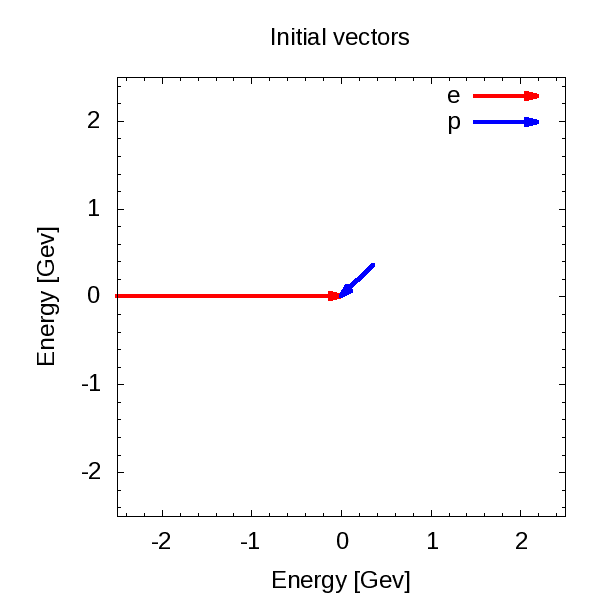
\includegraphics[width=8cm]{Initial.png}
\label{example}
\end{figure}

Using conservation of momentum and conservation of energy in elastic collisions, this simulation calculates the final state of the electron and proton after the scattering event by randomly selecting a scattered direction for the electron. The vector representation of the scattered products are shown in figure \ref{boom}. In order to make these calculations systematic and to study cross sections models the simulation transform each event into the rest frame of the target before scattering. 

\section{Transformation}
The Simulation completes a set of Lorentz invariant  rotations and boost for each event to transform the lab frame of the electron and proton collision into the rest frame of the proton. First the simulation takes the initial proton and electron vectors and rotates them to align the proton vector to the horizontal axis, shown in figure \ref{LAM}.This rotation uses the angle between the proton and the electron defined as $\lambda$. This allows for a straight forward calculations for the Lorentz factors $\beta$ and $\gamma $ and to boost into the rest frame of the target proton, figure \ref{boost}. Once in the boosted frame, the angle between the electron and the horizontal axis is defined as $\delta$.  Right before the simulation starts to calculate the scattered products, it completes one more rotation to align the electron vector with the horizontal axis, figure \ref{delta}, to make the scattering calculation systematic and unconditional. 

\begin{figure}[h]
  \centering
  
  \subfloat[Initial Vectors]{
  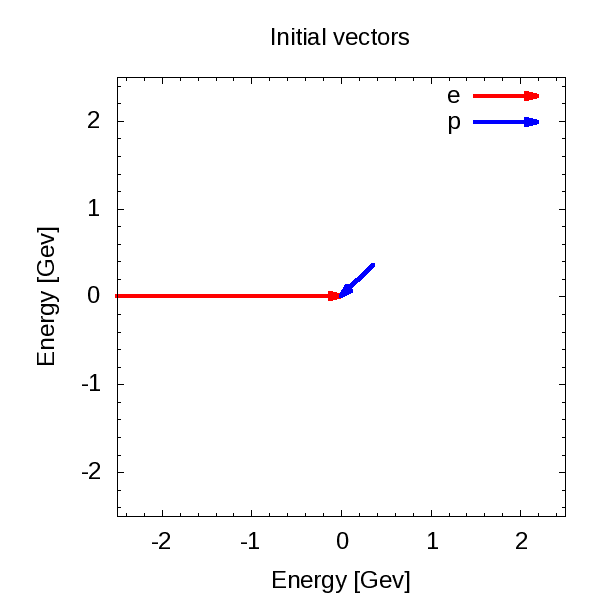
\includegraphics[width=6.5cm]{Initial.png}
  \label{IV}}
  \quad
  \centering
  \subfloat[Rotated by Lambda]{
  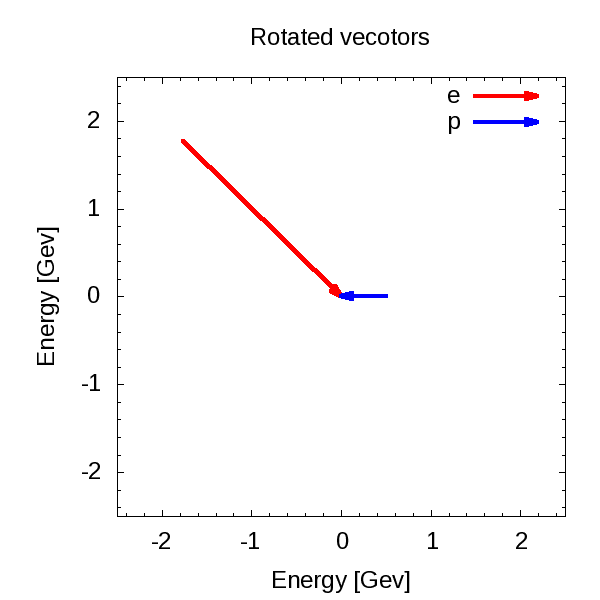
\includegraphics[width=6.5cm]{RotatedbyLam.png}
  \label{LAM}}
  \vspace{-2cm}
  \centering
  \subfloat[Boosted]{
  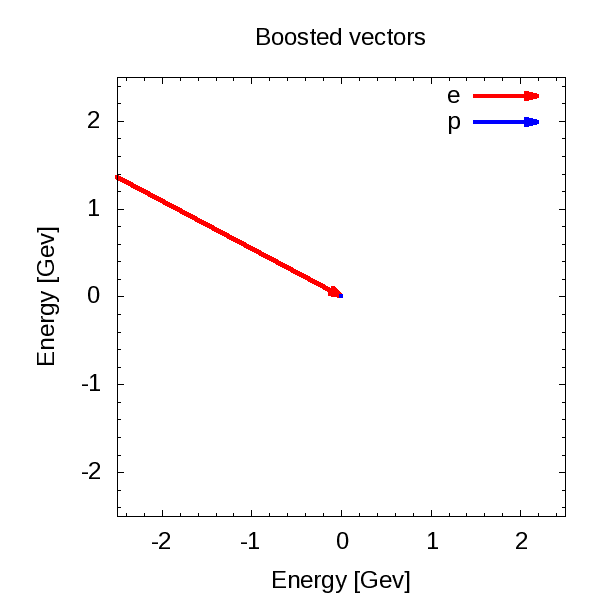
\includegraphics[width=6.5cm]{boosted.png}
  \label{boost}}
  \quad
  \centering
  \subfloat[Before being scattered]{
  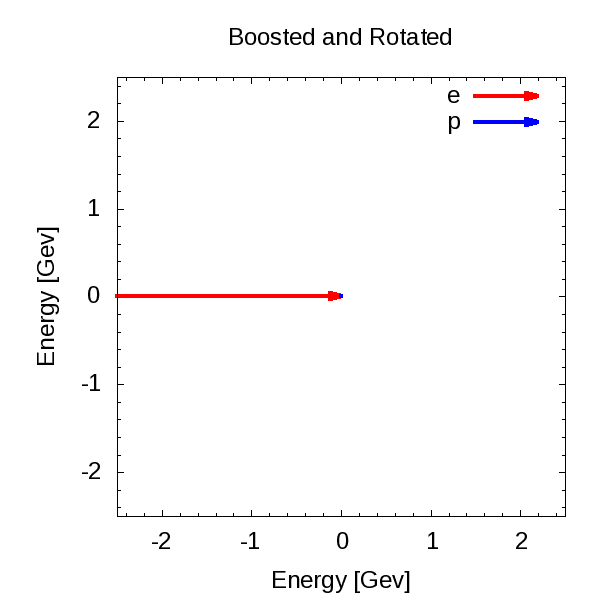
\includegraphics[width=6.5cm]{beforescattering.png}
  \label{delta}}
  
  \caption{Vector representations of the momentum for the incoming electron(red) and  target proton(blue) with units of GeV for each phase of their transformations before scattering.}
  \label{transform}
  \end{figure}
  
  In order to gain a more complete understanding of the scattering products, the program completes a set of transformations to move from the rest frame of the target proton to the beginning lab frame. After the simulation calculates the scattered products it begins to transform back by beginning with a rotation by the angle $\delta$, figure \ref{delta2}. Followed by the inverse of the previously used Lorentz boost. The last transformation, a rotation by $\lambda$, transforms the frame back into the lab frame. A proton vector and electron vector in the lab frame are the final products of the simulation. An image of the electron and proton vectors for each transformation can be found in figure \ref{transform2}. These vectors allow for calculation of kinematic variables such as Bjoken $x$ and the four-momentum transfer ($Q^2$).  This simulation will complete these steps for many electron and proton combinations.
  \begin{figure}[h]
    \centering
    \subfloat[After scattering]{
    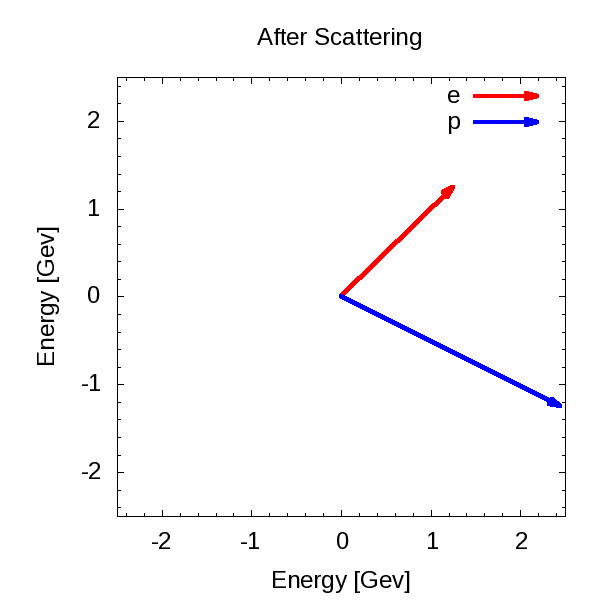
\includegraphics[width=6.0cm]{afterscatter.png}
    \label{boom}}
    \quad
    \centering
    \subfloat[Rotate back by $\delta$]{
    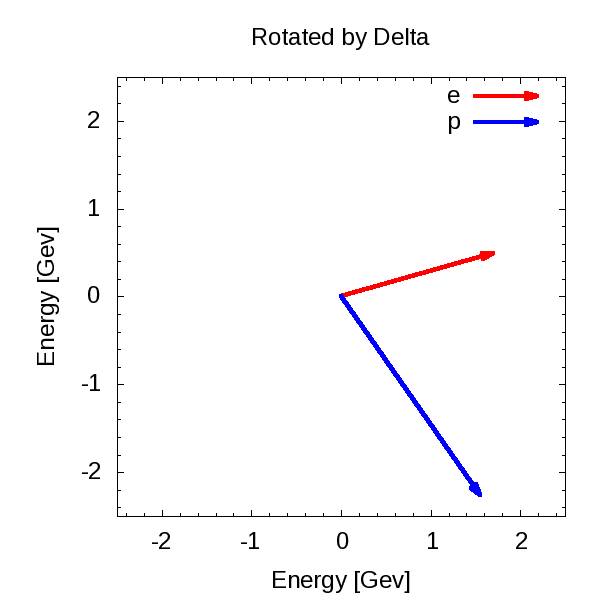
\includegraphics[width=6.0cm]{Rotatedbydelta.png}
    \label{delta2}}
    \vspace{-1cm}
    \centering
    \subfloat[Boosted]{
    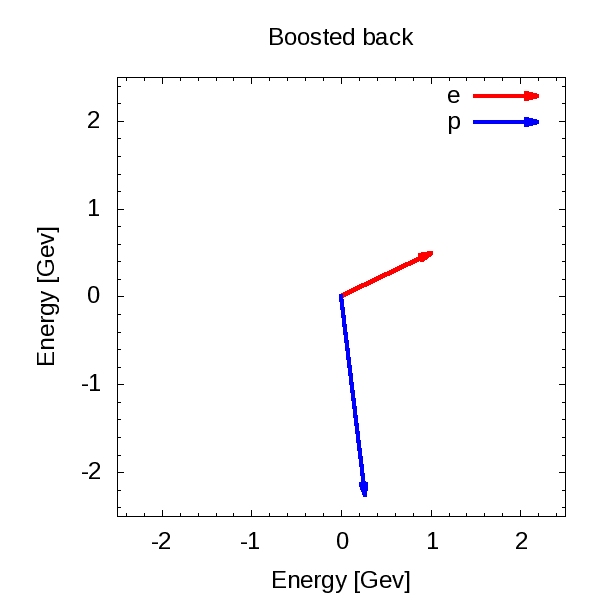
\includegraphics[width=6.0cm]{boostedback.png}
    \label{boost2}}
    \quad
    \centering
    \subfloat[Final vectors]{
   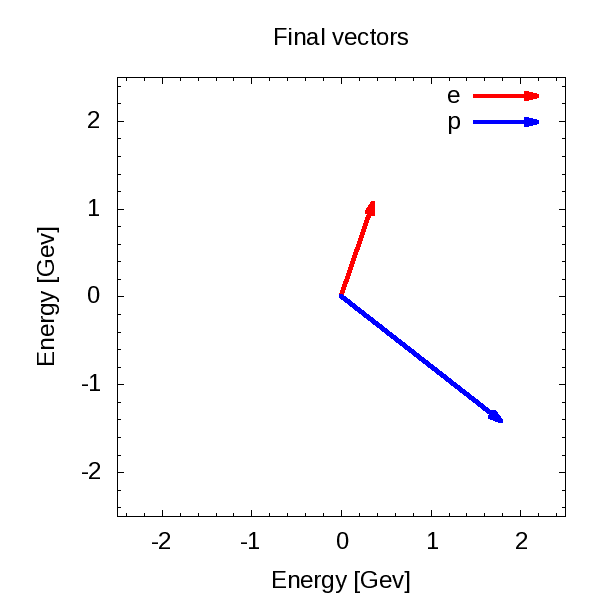
\includegraphics[width=6.0cm]{final.png}
    \label{Final}}
    
    \caption{Vector representations of the momentum for the incoming electron(red) and  target proton(blue) with units of GeV for each phase of their transformations after scattering).}
    \label{transform2}
    \end{figure}


\section{Results}
This electron scattering simulation produced results for two stages. The firsts stage used a fix proton momentum for each run to compare the yield in bins of $x_B$. Figure \ref{ES_res} shows the results for three different runs, each having a unique fixed proton momentum. The red histogram represents a run with a proton momentum of 0 Gev/c. The result is an elastic peak at $x_B$ of one. The blue histogram contains the results having a fixed proton momentum of 0.25 GeV/c. Increasing the initial momentum of the proton spreads the events into two peaks. The scattering interactions that form the peak above 1 $x_B$ are produced by events were the proton's initial directional vector are orientated towards the electron.  The events that produce an $x_B$ below 1 have a proton direction pointing away from the electron initially. Doubling the proton's initial momentum from 0.25 GeV to 0.50 GeV causes these peaks two spread out furtherer in $x_B$.  


\begin{figure}[h]
\centering
\caption{Simulation results for fixed momentum protons. Three runs with unique proton momentum. }
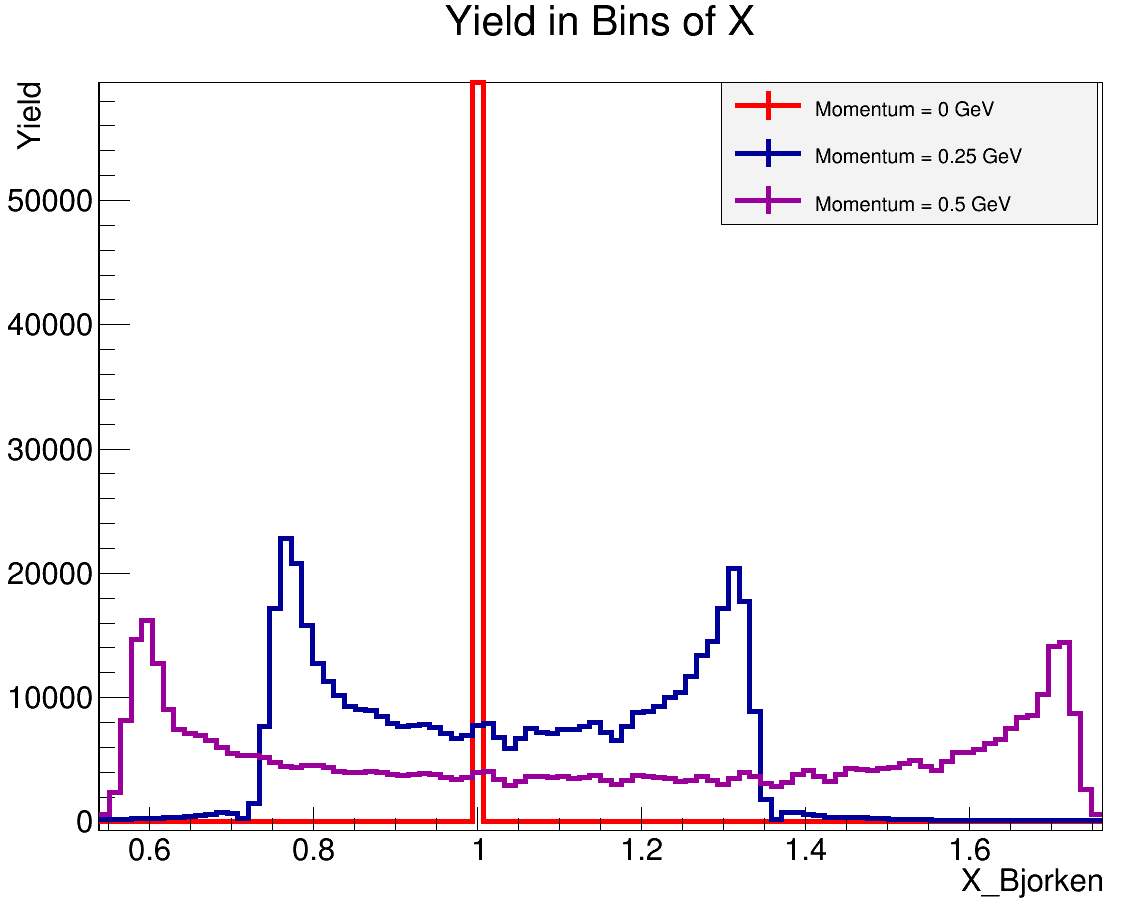
\includegraphics[width=15cm]{Es_results.png}
\label{ES_res}
\end{figure}


    	
\chapter{Conclusion}
\paragraph{}The MARATHON experiment took inclusive DIS data on the special designed sealed $^3$H cells, filled with $^3$H, $^3$He, and $^2$D at Thomas Jefferson National Accelerator Facility. The unique opportunity provided by access to $^3$H allowed the MARATHON experiment to be the first to use DIS to study the internal structure of this radioactive A=3 system. Alongside $^3$H, DIS data was taken on both $^3$He and $^2$D for ratio comparison. The experimental kinematics produces DIS events for $x$ from 0.18 to 0.8, with a Q$^2$ range of 3 to 12 (GeV$^2$) by rotating the electron spectrometer from 17.5 to 36 degrees and using the Continuous Electron Beam Accelerator Facility's 10.6 GeV beam. 
\paragraph{}The MARATHON data was used to produce result for the inclusive DIS cross section for these three gas targets. This measurement has provided the first extraction of the DIS cross section for $^3$H. Using the cross section measurements of the two A=3 mirror nuclei and $^2$D, the MARATHON collaboration has calculated the A=3 EMC effect for both $^3$He and $^3$H. This experiment will provide the first ever results on the EMC effect of $^3$H and the first on the comparison of the EMC effects of the two A=3 mirror nuclei. The MARATHON EMC effect for $^3$He agrees well with the previous JLab EMC measurement from experiment E03103 J. Seeley and A. Daniels \cite{seeley}. Due to this agreement, my analysis methods for the extraction of the EMC effect for $^3$He are validated, and therefore are valid for the extraction the EMC effect for $^3$H. The measurement of both the $^3$He and $^3$H EMC effects are important because comparison of the EMC measurements between these two A=3 nuclei can help evaluate isospin effects, and help remove model dependence of nuclear effects in the extraction of the $F^n_2/F^p_n$ structure function ratio. 

\paragraph{}The main goal of my analysis was to study the comparison of the EMC effect for the two A=3 mirror nuclei. I show the comparison of the EMC effect for $^3$H to the EMC effect for $^3$He in figure \ref{ISORatio}. This comparison shows no difference from unity within the precision of the current status of the analysis. 

\paragraph{}The biggest sources of error for the EMC effect are the isoscalar correction and cross section model dependence. The MARATHON's measurement of the $F^n_2/F^p_n$ ratio will help improve the errors associated with the isoscalar correction once the MARATHON collaboration finishes the analysis. The $F^n_2/F^p_n$ produced by a ratio of $^3$H and $^3$He will greatly reduce the error of the structure function ratio at high values of $x$ due to the small differences in nuclear effects in comparing the two A=3 mirror systems. A better understanding of the nucleon structure functions and the EMC effect will reduce the errors associated with the cross section extraction using a cross section model. Using an iterative procedure would help reduce the magnitude of the errors caused by the model dependence. A continuing goal of my analysis is to introduce an iterative procedure to correct the cross section model with data extracted cross sections. 

\paragraph{}The aim of this analysis is not to solve the EMC puzzle but too help find a pieces of the solution. The measurement of the EMC effect of $^3$H will add to the pool of previously measured nuclei that will continue to grow. A purposed experiment at Jefferson Lab plans to expand the database of known EMC effects by measuring the EMC effect on a large range of light and heavy nuclei \cite{pro_gaskell}. Another planed experiment at Jefferson Lab was proposed to provide new constraints on the EMC effect models by measuring the spin-dependent EMC effect on polarized $^7$Li \cite{pro_brooks}. Also, the flavor dependence of the EMC effect could be studied via pion induced Drell-Yan scattering\cite{Dutta} or tagged deep inelastic scattering measurements using the ALERT(Low Energy Recoil Tracker) detector in Hall B\cite{Armstrong}.



    %%%%%%%%%%%%%%%%%%%%%%%%%%%%%%%%%%%%%%%%%%%%%%%%%%%%%%%%%%%%%%%%%%%%%%%%%%%%%%%%%%%%%%%%%%%%%%%%%%%%%
    % BIBLIOGRAPHY
    %%%%%%%%%%%%%%%%%%%%%%%%%%%%%%%%%%%%%%%%%%%%%%%%%%%%%%%%%%%%%%%%%%%%%%%%%%%%%%%%%%%%%%%%%%%%%%%%%%%%%
    \makeBibliographyPage % make the bibliography title page - can be edited in ut-thesis-template.tex
    \bibliographystyle{plain} % bibliography style - recommend using apalike-doi as it hyperlinks DOIs
    \bibliography{references/references-dissertation} % references.bib included in the references directory
    %%%%%%%%%%%%%%%%%%%%%%%%%%%%%%%%%%%%%%%%%%%%%%%%%%%%%%%%%%%%%%%%%%%%%%%%%%%%%%%%%%%%%%%%%%%%%%%%%%%%%
    % APPENDIX - OPTIONAL - COMMENT IF NOT NEEDED
    %%%%%%%%%%%%%%%%%%%%%%%%%%%%%%%%%%%%%%%%%%%%%%%%%%%%%%%%%%%%%%%%%%%%%%%%%%%%%%%%%%%%%%%%%%%%%%%%%%%%%
    \makeAppendixPage   % make the appendix title page - can be edited in ut-thesis-template.tex
    \appendix
    

\section{Cross Section Tables}\label{CST}
\counterwithin{figure}{section}
\counterwithin{table}{section}
\paragraph{}This appendix contains the cross section tables for the three gas targets, $^3$H, $^3$He, and D. The data used to produce the cross section for these targets was acquired during the MARATHON experiment completed at JLab. The error for the three gas targets' thickness measurements are: $^3$H= 0.97\%, $^3$He = 1.12\%, and $^2$D = 0.56\% \cite{HATT_eng}. The errors contained in the table are the relative contribution to the cross section. The cuts used to produce the tables:

\textbf{Electron Selection Cuts}\\

\begin{tabular}{@{$\bullet$ }lcl}
	Number of tracks &==& 1\\
	MARATHON trigger (bit)  &\& &(1$<<$2)\\
	Total Cherenkov ADC sum &$>$ &1800\\
	Calo. Layer 1 Energy &$>$ & 1 GeV\\
	Calo. Layer 2 Energy &$>$ & 0.6 GeV\\
	W$^2$ &$>$ &2.5
\end{tabular}

\begin{tabular}{@{$\bullet$ }lcll}
	-0.07 m &$>=$& Vertex Z &$<=$ 0.09 m\\
	-0.035 &$ >=$ &$\delta_{tg}$ &$<=$ 0.035\\
	-0.04 rad &$>=$  &$\theta_{tg}$ &$<=$ 0.04 rad\\
	-0.025 rad &$>=$  &$\phi_{tg}$  &$<=$ 0.025 rad\\
\end{tabular}

\pagebreak
\newgeometry{hmargin=1in,vmargin=1in}
\thispagestyle{lscape}
\pagestyle{lscape}
\begin{landscape}

\begin{table}	
%\begin{sidewaystable}
\centering
\caption{Cross section table for $^3$H. }\label{CST_H3}
	\begin{tabular}{|p{1cm}|p{1cm}|p{1.5cm}|p{1.5cm}|p{2cm}|p{2cm}|p{1.5cm}|p{1.5cm}|p{2.5cm}|p{2.5cm}|}
		\hline
		x     & Q2     & Cross Section & Stat. Error & Density Cor. & Positron Sub. & Endcap Sub. & Detector Eff. & MC \& Model Error & Cross Section Error \\ \hline
		0.185 & 2.708  & 18.776        & 0.0055            & 0.002              & 0.0004               & 0.007              & 0.004                 & 0.016             & 0.019               \\ \hline
		0.215 & 3.055  & 15.49         & 0.0045            & 0.002              & 0.0002               & 0.007              & 0.004                 & 0.014             & 0.017               \\ \hline
		0.245 & 3.446  & 11.996        & 0.0049            & 0.002              & 0.0002               & 0.007              & 0.0041                & 0.013             & 0.016               \\ \hline
		0.275 & 3.881  & 8.617         & 0.0051            & 0.002              & 0.0001               & 0.007              & 0.0045                & 0.014             & 0.017               \\ \hline
		0.305 & 4.311  & 6.28          & 0.0059            & 0.002              & 0.0002               & 0.007              & 0.0051                & 0.014             & 0.018               \\ \hline
		0.335 & 4.705  & 4.931         & 0.0073            & 0.002              & 0.0002               & 0.007              & 0.0057                & 0.014             & 0.018               \\ \hline
		0.365 & 5.122  & 3.767         & 0.0082            & 0.002              & 0.0002               & 0.007              & 0.0067                & 0.014             & 0.019               \\ \hline
		0.395 & 5.55   & 2.794         & 0.0098            & 0.002              & 0.0002               & 0.007              & 0.0079                & 0.013             & 0.02                \\ \hline
		0.425 & 6.023  & 2.049         & 0.0091            & 0.002              & 0.0001               & 0.007              & 0.0091                & 0.013             & 0.02                \\ \hline
		0.455 & 6.397  & 1.591         & 0.009             & 0.002              & 0.0001               & 0.007              & 0.0091                & 0.013             & 0.02                \\ \hline
		0.49  & 6.922  & 1.153         & 0.01              & 0.002              & 0.0001               & 0.007              & 0.0083                & 0.013             & 0.02                \\ \hline
		0.53  & 7.472  & 0.776         & 0.0086            & 0.002              & 0.0001               & 0.007              & 0.0075                & 0.014             & 0.019               \\ \hline
		0.57  & 8.045  & 0.527         & 0.0111            & 0.002              & 0.0001               & 0.007              & 0.0071                & 0.016             & 0.022               \\ \hline
		0.61  & 8.617  & 0.351         & 0.0102            & 0.002              & 0.0001               & 0.007              & 0.0064                & 0.02              & 0.024               \\ \hline
		0.655 & 9.241  & 0.22          & 0.0115            & 0.002              & 0.0001               & 0.007              & 0.0055                & 0.025             & 0.029               \\ \hline
		0.705 & 9.997  & 0.121         & 0.0113            & 0.002              & 0.0                  & 0.007              & 0.0041                & 0.03              & 0.033               \\ \hline
		0.76  & 10.688 & 0.065         & 0.0109            & 0.002              & 0.0                  & 0.007              & 0.0035                & 0.026             & 0.029               \\ \hline
		0.825 & 11.468 & 0.03          & 0.0143            & 0.002              & 0.0                  & 0.007              & 0.0032                & 0.037             & 0.04                \\ \hline
	\end{tabular}
\end{table}
%\end{sidewaystable}
\end{landscape}
\restoregeometry
\pagestyle{plain}

\pagebreak
\newgeometry{hmargin=1in,vmargin=1in}
\thispagestyle{lscape}
\begin{landscape}

	\begin{table}
			\centering
	\caption{Cross section table for $^3$H.}\label{CST_He3}
	\begin{tabular}{|p{1cm}|p{1cm}|p{1.5cm}|p{1.5cm}|p{2cm}|p{2cm}|p{1.5cm}|p{1.5cm}|p{2.5cm}|p{2.5cm}|}
	\hline
	x     & Q2     & Cross Section & Stat. Error & Density Cor. & Positron Sub. & Endcap Sub. & Detector Eff. & MC \& Model Error & Cross Section Error \\ \hline
		0.185 & 2.709  & 20.71         & 0.0063            & 0.002              & 0.0006               & 0.007              & 0.004                 & 0.016             & 0.019               \\ \hline
		0.215 & 3.059  & 17.303        & 0.0051            & 0.002              & 0.0004               & 0.007              & 0.004                 & 0.015             & 0.018               \\ \hline
		0.245 & 3.447  & 13.59         & 0.0052            & 0.002              & 0.0002               & 0.007              & 0.0041                & 0.016             & 0.019               \\ \hline
		0.275 & 3.88   & 9.842         & 0.0056            & 0.002              & 0.0002               & 0.007              & 0.0044                & 0.017             & 0.02                \\ \hline
		0.305 & 4.313  & 7.22          & 0.0064            & 0.002              & 0.0002               & 0.007              & 0.0051                & 0.017             & 0.02                \\ \hline
		0.335 & 4.708  & 5.803         & 0.0074            & 0.002              & 0.0002               & 0.007              & 0.0058                & 0.017             & 0.021               \\ \hline
		0.365 & 5.122  & 4.446         & 0.0081            & 0.002              & 0.0002               & 0.007              & 0.0067                & 0.016             & 0.02                \\ \hline
		0.395 & 5.549  & 3.419         & 0.0095            & 0.002              & 0.0002               & 0.007              & 0.0079                & 0.015             & 0.021               \\ \hline
		0.425 & 6.024  & 2.499         & 0.009             & 0.002              & 0.0002               & 0.007              & 0.0091                & 0.014             & 0.02                \\ \hline
		0.455 & 6.397  & 1.974         & 0.0089            & 0.002              & 0.0002               & 0.007              & 0.0091                & 0.013             & 0.02                \\ \hline
		0.49  & 6.924  & 1.434         & 0.0098            & 0.002              & 0.0001               & 0.007              & 0.0083                & 0.012             & 0.019               \\ \hline
		0.53  & 7.473  & 0.985         & 0.0083            & 0.002              & 0.0001               & 0.007              & 0.0075                & 0.011             & 0.017               \\ \hline
		0.57  & 8.044  & 0.668         & 0.0108            & 0.002              & 0.0001               & 0.007              & 0.0071                & 0.013             & 0.02                \\ \hline
		0.61  & 8.616  & 0.447         & 0.0099            & 0.002              & 0.0001               & 0.007              & 0.0064                & 0.017             & 0.022               \\ \hline
		0.655 & 9.242  & 0.282         & 0.0112            & 0.002              & 0.0001               & 0.007              & 0.0055                & 0.024             & 0.028               \\ \hline
		0.705 & 9.998  & 0.158         & 0.0111            & 0.002              & 0.0001               & 0.007              & 0.0041                & 0.033             & 0.036               \\ \hline
		0.76  & 10.689 & 0.087         & 0.0105            & 0.002              & 0.0                  & 0.007              & 0.0035                & 0.035             & 0.037               \\ \hline
		0.825 & 11.467 & 0.038         & 0.0141            & 0.002              & 0.0                  & 0.007              & 0.0031                & 0.024             & 0.029               \\ \hline
	\end{tabular}
	\end{table}
\end{landscape}

\restoregeometry
\pagestyle{plain}

\pagebreak
\newgeometry{hmargin=1in,vmargin=1in}
\thispagestyle{lscape}
\begin{landscape}

	\begin{table}
			\centering
	\caption{Cross section table for D.}\label{CST_D2}
	\begin{tabular}{|p{1cm}|p{1cm}|p{1.5cm}|p{1.5cm}|p{2cm}|p{2cm}|p{1.5cm}|p{1.5cm}|p{2.5cm}|p{2.5cm}|}
	\hline
	x     & Q2     & Cross Section & Stat. Error & Density Cor. & Positron Sub. & Endcap Sub. & Detector Eff. & MC \& Model Error & Cross Section Error \\ \hline
		0.185 & 2.708  & 13.048        & 0.0062            & 0.002              & 0.0004               & 0.007              & 0.004                 & 0.015             & 0.018               \\ \hline
		0.215 & 3.061  & 10.858        & 0.0051            & 0.002              & 0.0002               & 0.007              & 0.004                 & 0.013             & 0.016               \\ \hline
		0.245 & 3.452  & 8.473         & 0.0051            & 0.002              & 0.0002               & 0.007              & 0.0041                & 0.013             & 0.016               \\ \hline
		0.275 & 3.883  & 6.147         & 0.0049            & 0.002              & 0.0001               & 0.007              & 0.0045                & 0.014             & 0.017               \\ \hline
		0.305 & 4.31   & 4.596         & 0.0053            & 0.0024             & 0.0002               & 0.007              & 0.0051                & 0.015             & 0.018               \\ \hline
		0.335 & 4.695  & 3.724         & 0.0066            & 0.0027             & 0.0002               & 0.007              & 0.0055                & 0.015             & 0.019               \\ \hline
		0.365 & 5.119  & 2.812         & 0.0083            & 0.0033             & 0.0001               & 0.007              & 0.0064                & 0.015             & 0.02                \\ \hline
		0.395 & 5.549  & 2.111         & 0.0119            & 0.004              & 0.0001               & 0.007              & 0.0079                & 0.014             & 0.022               \\ \hline
		0.425 & 6.023  & 1.574         & 0.0115            & 0.003              & 0.0001               & 0.007              & 0.0091                & 0.014             & 0.022               \\ \hline
		0.455 & 6.397  & 1.279         & 0.0112            & 0.003              & 0.0001               & 0.007              & 0.0091                & 0.013             & 0.021               \\ \hline
		0.49  & 6.944  & 0.868         & 0.0113            & 0.003              & 0.0001               & 0.007              & 0.0081                & 0.013             & 0.021               \\ \hline
		0.53  & 7.474  & 0.615         & 0.0083            & 0.003              & 0.0001               & 0.007              & 0.0075                & 0.012             & 0.018               \\ \hline
		0.57  & 8.045  & 0.427         & 0.0106            & 0.003              & 0.0001               & 0.007              & 0.0071                & 0.014             & 0.02                \\ \hline
		0.61  & 8.615  & 0.286         & 0.0096            & 0.003              & 0.0                  & 0.007              & 0.0064                & 0.017             & 0.022               \\ \hline
		0.655 & 9.239  & 0.179         & 0.011             & 0.003              & 0.0                  & 0.007              & 0.0055                & 0.022             & 0.026               \\ \hline
		0.705 & 9.992  & 0.098         & 0.011             & 0.0026             & 0.0                  & 0.007              & 0.0041                & 0.028             & 0.031               \\ \hline
		0.76  & 10.688 & 0.052         & 0.0109            & 0.0022             & 0.0                  & 0.007              & 0.0035                & 0.027             & 0.03                \\ \hline
		0.825 & 11.467 & 0.023         & 0.0143            & 0.002              & 0.0                  & 0.007              & 0.0032                & 0.026             & 0.031               \\ \hline
	\end{tabular}
	\end{table}
\end{landscape}
\restoregeometry
\pagestyle{plain}
    %%%%%%%%%%%%%%%%%%%%%%%%%%%%%%%%%%%%%%%%%%%%%%%%%%%%%%%%%%%%%%%%%%%%%%%%%%%%%%%%%%%%%%%%%%%%%%%%%%%%%
    % A VITA IS REQUIRED
    %%%%%%%%%%%%%%%%%%%%%%%%%%%%%%%%%%%%%%%%%%%%%%%%%%%%%%%%%%%%%%%%%%%%%%%%%%%%%%%%%%%%%%%%%%%%%%%%%%%%%
    \addToTOC{Vita}
    % resume.tex
% vim:set ft=tex spell:



\setlength{\tabcolsep}{0em}



\lfoot{Jason Bane}


% indentsection style, used for sections that aren't already in lists
% that need indentation to the level of all text in the document
\newenvironment{indentsection}[1]%
{\begin{list}{}%
		{\setlength{\leftmargin}{#1}}%
		\item[]%
	}
	{\end{list}}

% opposite of above; bump a section back toward the left margin
\newenvironment{unindentsection}[1]%
{\begin{list}{}%
		{\setlength{\leftmargin}{-0.5#1}}%
		\item[]%
	}
	{\end{list}}

% format two pieces of text, one left aligned and one right aligned
\newcommand{\headerrow}[2]
{\begin{tabular*}{\linewidth}{l@{\extracolsep{\fill}}r}
		#1 &
		#2 \\
\end{tabular*}}

% make "C++" look pretty when used in text by touching up the plus signs
\newcommand{\CPP}
{C\nolinebreak[4]\hspace{-.05em}\raisebox{.22ex}{\footnotesize\bf ++}}

\begin{center}
{\large \textbf{Vita}}\\
{\large \textbf{Jason Bane}}

\end{center}

\hrule
\vspace{-0.4em}
\subsection*{Education}

\begin{itemize}
\parskip=0.1em

\item 
\headerrow
{\textbf{University of Tennessee}}
{\textbf{Knoxville, TN}}

\headerrow
{\emph{Ph.D. in Nuclear Physics}}
{\emph{August 2012 -- Planned December 2019}}
\headerrow
{\emph{Thesis: The EMC Effect in A=3 Nuclei}}
{\emph{Advisor: Nadia Fomin}}
%	\begin{itemize*}
%		\item Lorem ipsum dolor sit amet, consectetuer adipiscing elit.
%		\item Mirum est notare quam littera gothica, quam nunc putamus parum
%		claram.
%	\end{itemize*}


\parskip=0.1em

\item 
\headerrow
{\textbf{University of Tennessee}}
{\textbf{Knoxville, TN}}
\\
\headerrow
{\emph{Secondary Education Certification in Math and Science}}
{\emph{August 2009 -- May 2010}}
%	\begin{itemize*}
%		\item Lorem ipsum dolor sit amet, consectetuer adipiscing elit.
%		\item Mirum est notare quam littera gothica, quam nunc putamus parum
%		claram.
%	\end{itemize*}


\parskip=0.1em

\item 
\headerrow
{\textbf{University of Tennessee}}
{\textbf{Knoxville, TN}}
\\
\headerrow
{\emph{Bachelor of Science, Physics \& Minor in Education }}
{\emph{August 2004 -- May 2009}}

%	\begin{itemize*}
%		\item Lorem ipsum dolor sit amet, consectetuer adipiscing elit.
%		\item Mirum est notare quam littera gothica, quam nunc putamus parum
%		claram.
%	\end{itemize*}

\end{itemize}
\hrule
\vspace{-0.4em}
\subsection*{Experience}

\begin{itemize}
\parskip=0.1em

\item
\headerrow
{\textbf{University of Tennessee}\\\textbf{Department of Physics and Astronomy }}
{\textbf{  Knoxville, TN,}}
\\
\headerrow
{\emph{Graduate Research Assistant }}
{\emph{May 2014 -- Present}}
\begin{itemize}
	\item Designed and constructed front end electronics for an electron spectrometer.
	\item Created module layouts and cable maps for efficient reuse of products.
	\item Tested high voltage cards and laid high voltage cable for an electron spectrometer.
	\item Used Oscilloscopes to test signals, debug logic modules, and map out inconsistent signals.  
	\item Maintained and refurbished individual detector components of a spectrometer including checking the quality of Photo Multiplier Tubes and plastic scintillators.
	\item Calibrated detectors and used online analysis tools in Java to control the quality of data during shifts for an experiment. 
	\item Performed analysis on a large set of data involving multiple nuclear targets using Python, C++ , ROOT, and fortran. 
	\item Worked with a diverse collaboration, leading projects and working as a team member
\end{itemize}
\vspace{0.85cm}
\item
\headerrow
{\textbf{University of Tennessee}\\\textbf{Department of Physics and Astronomy }}
{\textbf{  Knoxville, TN,}}
\\
\headerrow
{\emph{Graduate Teaching Assistant }}
{\emph{August 2012 -- May 2015}}
\begin{itemize}
	\item Designed and implemented observational and planetarium based astronomy labs.
	\item Educated students on the use of refracting telescopes and equatorial mounts.
	\item Instructed students in laboratory exercises to help conceptualize physics topics.
	\item Tutored students for homework assistance and test prep.
\end{itemize}
\begin{samepage}
	\item
	\headerrow
	{\textbf{Clay County Tennessee Education Department}}
	{\textbf{Celina, TN}}
	\\
	\headerrow
	{\emph{Secondary Educator \& Football Coach}}
	{\emph{August 2010 -- May 2012 }}
	\begin{itemize}
		\item Created lesson plans that included interactive, creative thinking, and discussion driven curriculum for a diverse body of geometry students.
		\item Constructed lessons that used hands-on lab activities, demonstrations, and interactive computer lessons to instruct high school Juniors and Seniors in algebra-based physics. 
		\item Used discussion-based problem-solving lessons to help remedial math students to improve their algebra, geometry and trigonometry skills for post-secondary education. 
		\item Provided an equitable and inclusive atmosphere for diverse students. 
		\item Math and reading focused tutoring. 
	\end{itemize}
\end{samepage}
\end{itemize}




\hrule
\vspace{-0.4em}
\subsection*{Core Technical Skills}

\begin{indentsection}{\parindent}
\hyphenpenalty=1000
\begin{description}
	\item[Hardware:]
	Detector maintenance and wiring, front end electronics design and implementation, logical trigger design and testing   
	\item[Languages:]
	C, \CPP, \LaTeX, Python, shell script, SQL \\
	Monte Carlo Simulation Packages\\
	Example scripts located at https://github.com/jbane11/examples
	\item[Software:]
	Microsoft Office, Libre Office, Texstudio, vim, atom
	\item[Operating Systems:]
	Linux(Red Hat), Windows, MacOS
	
\end{description}
\end{indentsection}
\hrule
\subsection*{Publications}
\begin{itemize} \itemsep -2pt % Reduce space between items
\item  H. Dai, [et al. including \textbf{J. Bane}], ``First Measurement of the Ar(e,$e^\prime$)X Cross Section at Jefferson Lab," Phys. Rev. C 99, 054608 May 2019
\item R. Cruz-Torres, [et al. including \textbf{J. Bane}], ``Comparing proton momentum distributions in A=3 nuclei via $^3$He and $^3H$(e,$e^\prime$p) measurements," in preparation, (2019)
\item S. N. Santiesteban, S. Alsalmi, D. Meekins, \textbf{J. Bane,} et al., ``Density Changes in Low Pressure Gas Targets for Electron Scattering Experiments" NIM A 940, 2019
\item  H. Dai, [et al. including \textbf{J. Bane}], ``First Measurement of the Ti(e,$e^\prime$)X Cross Section at Jefferson Lab," Phys. Rev. C 98, 014617 July 2018
\item P V. Pandey, [et al. including \textbf{J. Bane}], ``Probing electron-argon scattering for liquid-argon based neutrino-oscillation program," preprint arXiv:1711.01671

\end{itemize}
\hrule
\subsection*{Honors}
\begin{itemize}
\item Jefferson Science Associates graduate fellowship award (2018)  
\item Chancellor’s honors for extraordinary professional promise (2016) 
\item DOE Office of Science Graduate Student Research program award (2015)
\item Dean's List 2009 Academic Year (2010)
\end{itemize}
\hrule
\subsection*{Conference Presentations}
\begin{itemize}
\item F$_2$ ratio and EMC effect for A=3 Mirror Nuclei", 24th European Conference on Few-body Problems in Physics, University of Surrey, England, September 2019.
\item "EMC in A=3 from MARATHON," 2nd Workshop on Quantitative Challenges in SRC and EMC Research,  MIT, Cambridge MA,  March 2019
\item "Ratios in A=3 nuclei from MARATHON ," American Physical Society's Division of Nuclear Physics' yearly meeting, HA, October 2018
\item "Measurement of the spectral function of Argon and Titanium through the(e,$e^\prime$p) reaction," American Physical Society's Division of Nuclear Physics' yearly meeting, HA, October 2018
\item "Status of the MARATHON experiment." American Physical Society's Division of Nuclear Physics' yearly meeting, Pittsburgh PA, October 2017
\item "Searching for the Origin of the EMC effect." American Physical Society's Division of Nuclear Physics' yearly meeting, Sante Fe NM, October 2016
\end{itemize}

\hrule
\subsection*{Poster Presentations}
\begin{itemize}
\item "The impetus in the EMC effect, a EMC simulation." Gordon Research Conferences, Holderness, NH. August 2018 
\item "Searching for the Origin of the EMC effect." SURA Board of Trustees Meeting, Newport News, VA. April 2018 
\end{itemize}

\hrule

\subsection*{Interests}

Football, coaching, programming, boating, traveling,




\end{document}
